\chapter{模式与出发时间选择方法的训练与评估}

建立好深度强化学习模型后,进行训练和评价对模型的发展和应用具有重大意义。这一过程可以从多方面优化模型性能,为模型在实际应用中的选用提供依据。首先,训练和评价过程可以验证模型的有效性,确保模型能够有效解决所面临的问题。训练过程使智能体学会最优策略,而评价过程则有助于了解模型在实际应用场景中的性能表现。其次,训练和评价过程有助于提高模型性能。智能体在训练过程中持续优化神经网络参数,提高任务表现。评价过程揭示了模型在某些方面的不足,为进一步优化提供线索。训练和评价过程还可以揭示不同算法在特定任务上的优劣,为实际应用中的算法选择提供依据。同时,对现有模型的训练和评价可以发现算法存在的问题和不足,激发新的算法研究和改进,进而推动深度强化学习领域的发展。总之,建立好模型后的训练和评价过程不仅能全面了解模型性能表现,提高泛化能力,优化参数设置,还能为算法选择和领域研究提供重要支持。


在本章中,将对上一章中提出的基于深度强化学习的出行模式与时间选择模型进行训练,并对训练结果进行详细分析,以了解模型的收敛速度和稳定性。此外,本章还将对模型进行评估,包括与传统方法的对比和模型参数的灵敏性分析,以验证模型的有效性。


\section{模型的训练与分析}

在本节中,将对上一章提出的算法模型进行训练,并对训练结果进行详细分析。通过观察训练过程中的学习曲线和计算累积奖励,可以深入了解模型在训练过程中的性能变化和整体表现。学习曲线和累积奖励作为评估深度强化学习模型表现的关键指标,能够从多方面反映模型性能。学习曲线揭示了模型在训练过程中的性能变化,有助于判断模型收敛速度和稳定性;累积奖励则反映智能体在任务中的整体表现,可以用于比较不同模型或算法的相对性能优劣。此外,这些指标还有助于评估模型的泛化能力和算法效率。观察学习曲线和累积奖励在训练集与测试集上的表现,可以判断模型是否适应新环境;同时,学习曲线还能反映算法在训练过程中的效率差异。因此,这些指标为模型优化、算法选择和参数调整提供了重要依据。

\subsection{实验场景的设置}

在训练之前,先确定一系列仿真参数来构建训练模型的场景。表\ref{public}列出了数值实验中使用的各个参数及其描述和取值。这些参数反映了不同出行方式的特点,如公交车和地铁的票价、运行频率和停留时间等。此外,还包括了如时间价值、提前到达和迟到的时间表延误成本等与个体出行决策相关的因素。
\renewcommand{\arraystretch}{1.2}
\setlength{\tabcolsep}{8mm}
\begin{table}[htbp]
\centering
\caption{实验中使用的仿真参数取值}
\label{public}
\begin{tabular}{lcl}
\toprule
参数 & 描述                                                 & 数值 \\ 
\midrule
$t_\text{min}$  & 最早出发时间                                     & 07:00 \\
$t_\text{max}$  & 最晚出发时间                                     & 09:00 \\
$t_\text{unit}$  & 出发时间选择的单位间隔(分钟)                   & 30    \\
$E_1$  & 将成本映射到奖励的常数                               & 100   \\
$E_2$  & 将成本映射到奖励的常数                               & 0.1   \\
$\alpha$  & 时间价值(元/分钟)                               & 0.5   \\
$\beta$  & 提前到达的时间表延误的单位成本(元/分钟)           & 0.05  \\
$\gamma$  & 迟到的时间表延误的单位成本(元/分钟)             & 0.3   \\
$o$  & 燃油价格(元/公里)                                 & 0.56  \\
\textbackslash{}  & 公交票价(元)                             & 2     \\
\textbackslash{}  & 地铁起步票价(元)                         & 1     \\
\textbackslash{}  & 地铁每公里递增票价(元/公里)               & 0.2   \\
\textbackslash{}  & 公交高峰频率(辆/小时)                      & 10    \\
\textbackslash{}  & 地铁高峰频率(辆/小时)                      & 14    \\
\textbackslash{}  & 公交非高峰频率(辆/小时)                    & 6     \\
\textbackslash{}  & 地铁非高峰频率(辆/小时)                    & 8     \\
\textbackslash{}  & 公交停留时间(秒)                           & 40    \\
\textbackslash{}  & 地铁停留时间(秒)                           & 30    \\ 
\bottomrule
\end{tabular}
\end{table}



\subsection{智能体的聚类与选取}


选择60个具有时间依赖性的起点-终点(OD)出行旅程作为智能体选取的样本集,并将它们的旅行特征输入到聚类方法中。表\ref{tab:sample_all}为部分出行的相关信息,包含出行ID,出发时间,出发路段,到达路段,与公共交通的可达性。

\renewcommand{\arraystretch}{1.2}
\begin{table}[htbp]
\centering
\caption{智能体部分样本数据示例}
\label{tab:sample_all}
\small % Adjust font size here
\setlength{\tabcolsep}{4pt} % Adjust column spacing here

\begin{tabular}{cccccc}
\toprule
出行ID & 出发时间[s]  &    出发路段         &到达路段 &行程距离[km]   & 可达性[km] \\ 
\midrule
1	& 76	& 912\@941\#0 &	922\@772\#0 &	6.37&	1.48 \\
2	& 267 &	109\@758\#0 & 	673\@925\#0 &	2.89&	0.89 \\
3	& 331 &	76\@760\#0&	98\@918\#0&	5.56&	1.89\\
4&	0&	818\@890\#0&	27\@601\#0	&4.21	&1.93   \\
...&	...&	...&	...&...	&...   \\
60&	18&	818\@890\#0&	819\@24\#0&	3.41&	0.32  \\
\bottomrule
\end{tabular}
\end{table}



在实施DBSCAN算法的过程中,需要确定两个关键参数:邻域半径($\mu$)和最小样本数($m$)。邻域半径的选取至关重要,因为它决定了算法认定哪些点属于同一个簇。如果两个点之间的距离小于邻域半径,那么就认为这两个点属于同一个簇。另一个关键参数是最小样本数,它表示一个簇中至少需要包含$m$个样本才能被认定为有效簇。这两个参数的选择会直接影响到聚类结果的质量,因此需要慎重考虑。

在本研究中,选择了经验法来确定DBSCAN算法的参数。经验法是一种依赖于经验或常识的方法,通过手动调整邻域半径和最小样本数的值来寻找最佳参数组合。首先尝试了不同的邻域半径和最小样本数组合,同时记录每种组合的轮廓系数得分。轮廓系数是一种用于评估聚类结果质量的指标,其值介于$-1$和$1$之间。计算轮廓系数的方法是将一个样本的簇内平均距离($a$)与与其最近簇的所有样本的簇内平均距离($b$)进行比较,计算得出该样本的轮廓系数为${(b-a)} / {max(a,b)}$,然后计算所有样本的轮廓系数的平均值。轮廓系数越接近1,说明聚类效果越好;越接近-1,说明聚类效果较差。

为了展示这一过程,表\ref{tab_cluster}呈现了尝试过的不同参数组合及其对应的轮廓系数得分。这有助于选择出最佳参数组合,从而提高聚类结果的质量。通过这种方法,可以确保在处理具有代表性的个体时,采用了较为合适的聚类参数。

\renewcommand{\arraystretch}{1.2} % 使表格行间距加大1.5倍
\setlength{\tabcolsep}{8mm}
\begin{table}[htbp]
\centering
\caption{参数组合及轮廓系数得分表}
\label{tab_cluster}
\begin{tabular}{ccc}
\toprule
邻域半径 ($\mu$) & 最小样本数 ($m$) & 轮廓系数得分       \\
\midrule
0.3 & 2 & 0.75 \\ 
0.3 & 3 & 0.72 \\ 
0.5 & 2 & 0.82 \\ 
0.5 & 3 & 0.79 \\ 
0.7 & 2 & 0.76 \\ 
0.7 & 3 & 0.74 \\ 

\bottomrule
\end{tabular}
\end{table}

通过实验,发现最佳参数组合为邻域半径为0.5,最小样本数为2。在这个参数组合下,得到的轮廓系数为0.82,表明聚类效果良好。将最小点数设置为10和最小距离阈值设置为0.05,共得到了4个类别以及2个噪声点,聚类的结果如图\ref{db_cluster}所示,图中标识的4个代表点将作为代表智能体,在训练时其经验被放入公共记忆池中。
\begin{figure}[H]
  \centering
  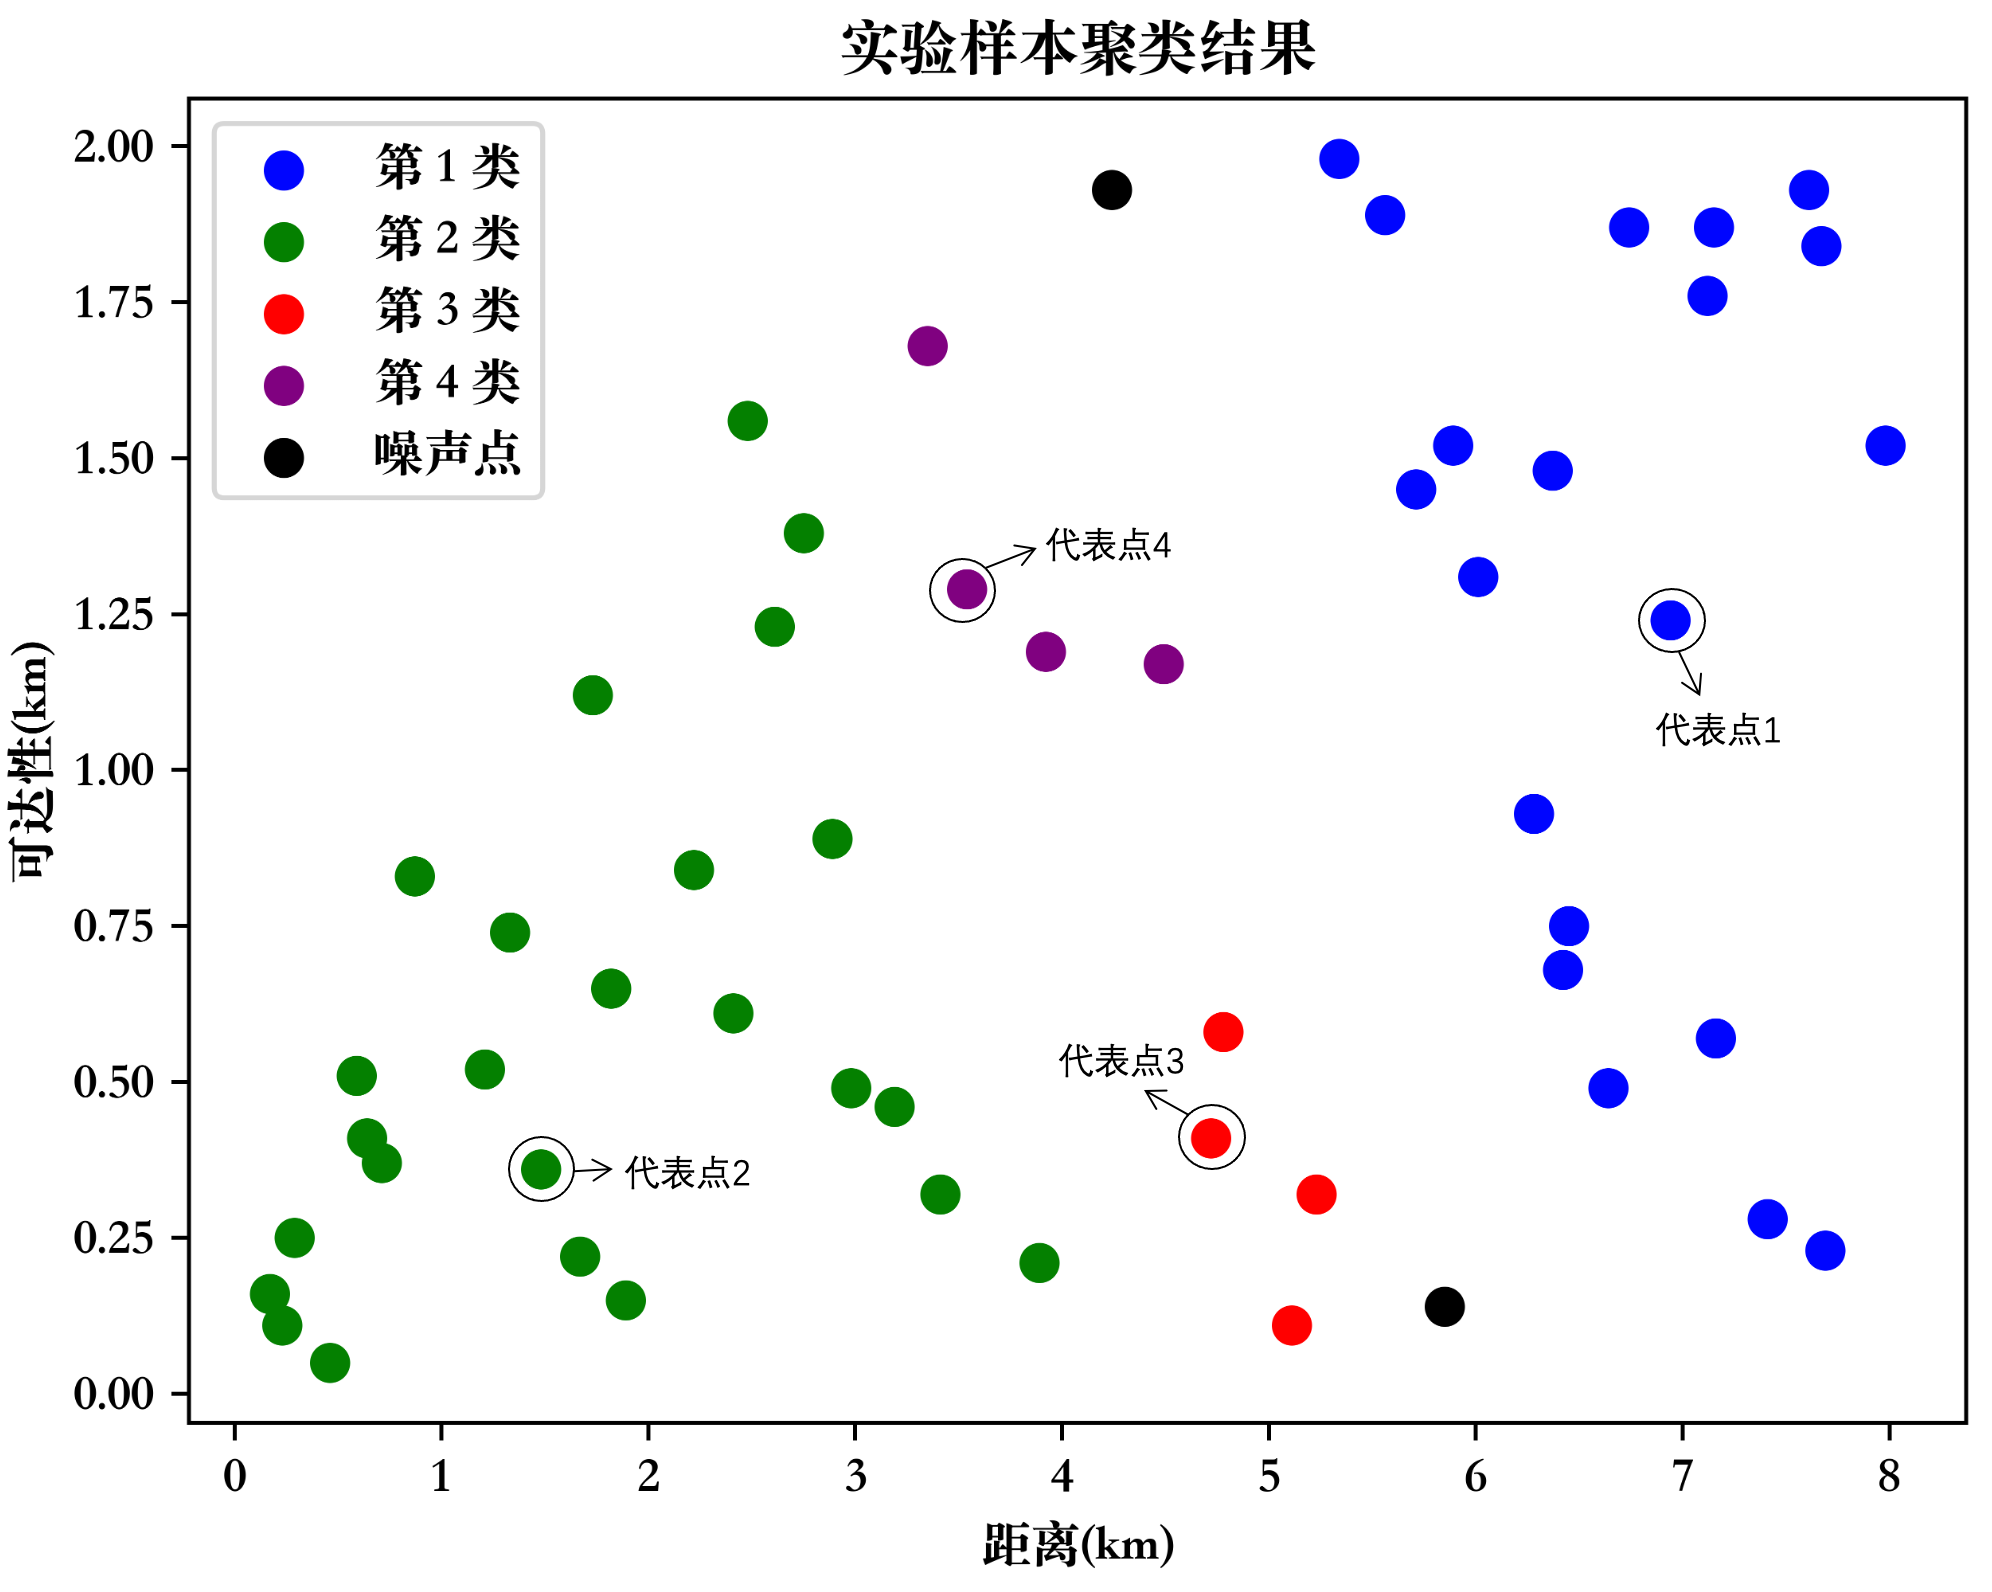
\includegraphics[width=.75\linewidth]{figures/content/db_cluster.png}
  \caption{代表智能体的位置示意图}
  \label{db_cluster}
\end{figure}


\subsection{训练及结果分析}

在本文中,采用深度Q网络算法来优化出行模式和出发时间的选择,以获得最佳的出行体验。有数值实验均在标准计算机上进行,配置为Intel Core (TM) i5-9400F 2.90 GHz CPU和8 GB RAM。将训练过程设置为800个episode。在每个时间步长内,智能体根据当前状态选择一个动作,然后接收到环境返回的奖励,并转移到下一个状态。我们使用$\varepsilon$-贪婪策略来探索动作空间,其中$\varepsilon$在前400个episode中线性下降到0.1,然后保持不变。在探索时,智能体将以$\varepsilon$的概率选择一个随机动作,否则将根据当前Q值估计选择一个最佳动作。

使用SUMO仿真工具来模拟城市交通网络,四个代表智能体的OD在网络中的位置如图\ref{agent_map}所示,将智能体的行为应用于仿真中的出行模式选择和出发时间选择中。根据仿真结果,可以获得出行时间、路线和交通方式等方面的信息,以评估该算法的性能。
\begin{figure}
  \centering
  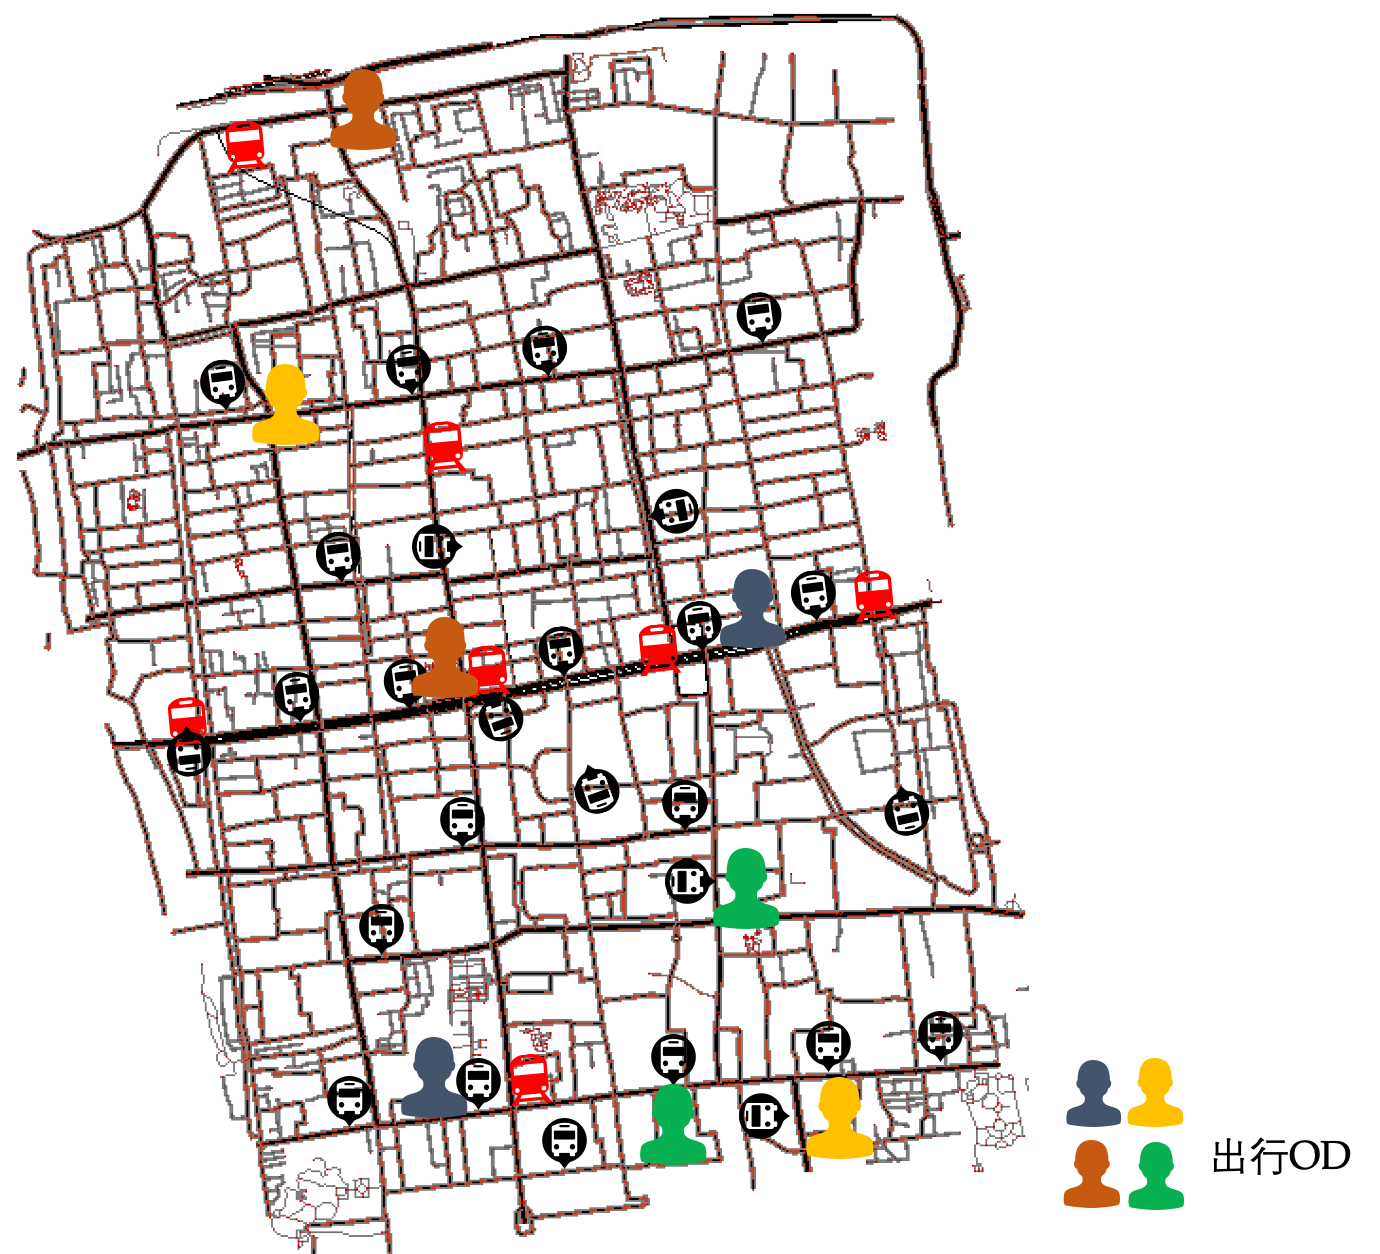
\includegraphics[width=.75\linewidth]{figures/content/agent_map.png}
  \caption{代表智能体的位置示意图}
  \label{agent_map}
\end{figure}

首先,在训练过程中设置了一个经验回放机制。该机制用于存储代理在仿真环境中所经历的状态、动作、奖励和下一状态等信息,并且按照一定的概率进行抽样,以保证数据的独立性和随机性。其次,采用目标网络的方法来减小估计误差的影响。在训练过程中使用了两个神经网络,即一个本地网络和一个目标网络。本地网络用于根据当前状态计算Q值,而目标网络则用于计算目标Q值。在一定的时间间隔内,目标网络的参数会从本地网络中更新,以缓解估计误差的影响。最后,将使用Adam优化器来对网络进行训练,以提高算法的收敛速度和性能。

图 \ref{loss&reward} 显示了在训练800个周期中损失值和奖励值的收敛模式变化。在损失值变化图像中,整体呈现出明显的下降趋势,这与期望相符。在训练初期,由于智能体在训练开始阶段需要对环境进行行动探索,因此损失函数值波动较大。然而,这种波动主要集中在前300个周期,并且持续时间相对较短。实际上,从大约第500个周期开始,损失函数值的变化微小,几乎呈直线趋势。这一观察结果明确地证实了算法的收敛性。从图中可以看出,本文提出的深度强化学习算法在训练过程中表现良好,并已在此任务上达到收敛。为了评估算法在此任务上的性能,可以计算平均奖励值。在训练过程中,每个代表个体通过遵循深度强化学习推荐的行动所获得的奖励的变化结果如图 \ref{loss&reward}(b)所示。考虑到每个代表个体的旅行都具有不同的OD,相关的奖励大小也不同。事实上,可以轻易地发现,智能体1可能会有最长的旅行,而智能体3和4可能会有较短的旅行。然而,无论奖励的绝对值如何,所有代表个体的曲线都呈现出增长的趋势,这意味着他们通过与环境的交互并学习不断改进他们的旅行选择。在大约700个阶段内,每个代表的奖励基本稳定,并且此后变化不大,这一观察结果与图 \ref{loss&reward}(a)一致。图 \ref{loss&reward} 的结果表明,通过使用深度强化学习,智能体能够有效地学习并逐渐改善其决策。在训练过程中,智能体能够对环境进行探索,并通过与环境的交互学习如何选择最优的行动,从而最小化旅行时间和出行成本。此外,随着训练周期的增加,智能体的学习能力逐渐提高,同时收敛速度也变得更快。
\begin{figure}
\centering
  \subfloat[损失值变化图像]{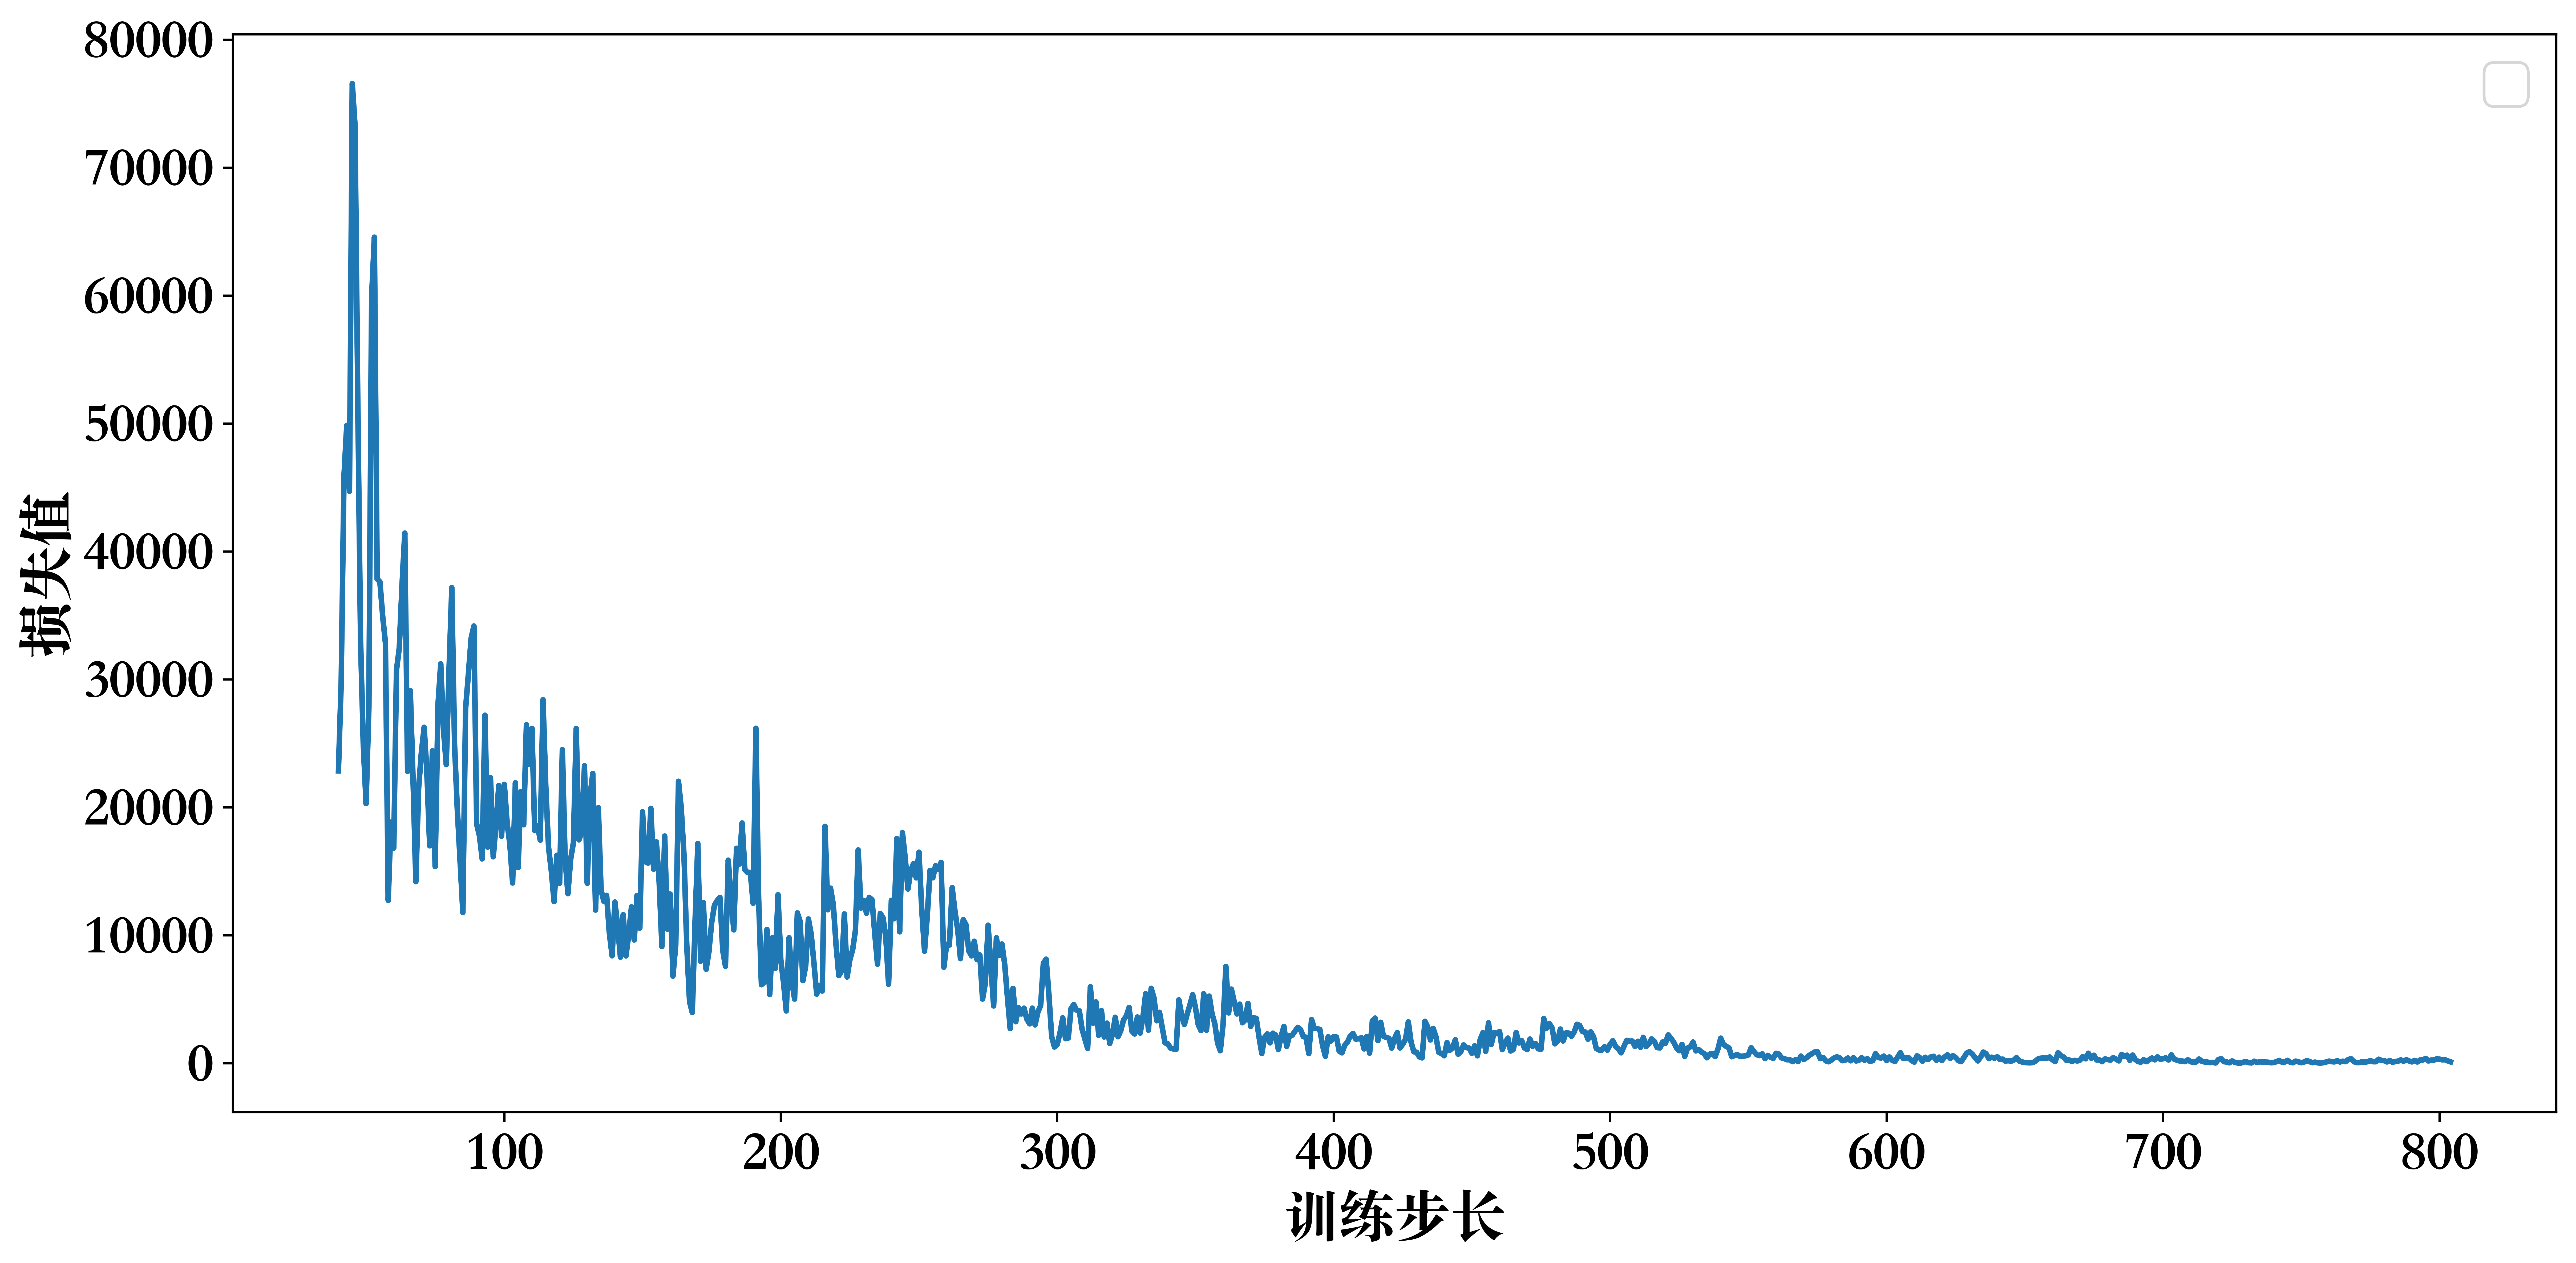
\includegraphics[width=.85\textwidth]{figures/content/loss.png}}
  \label{loss}
  \\
  \subfloat[奖励变化图像]{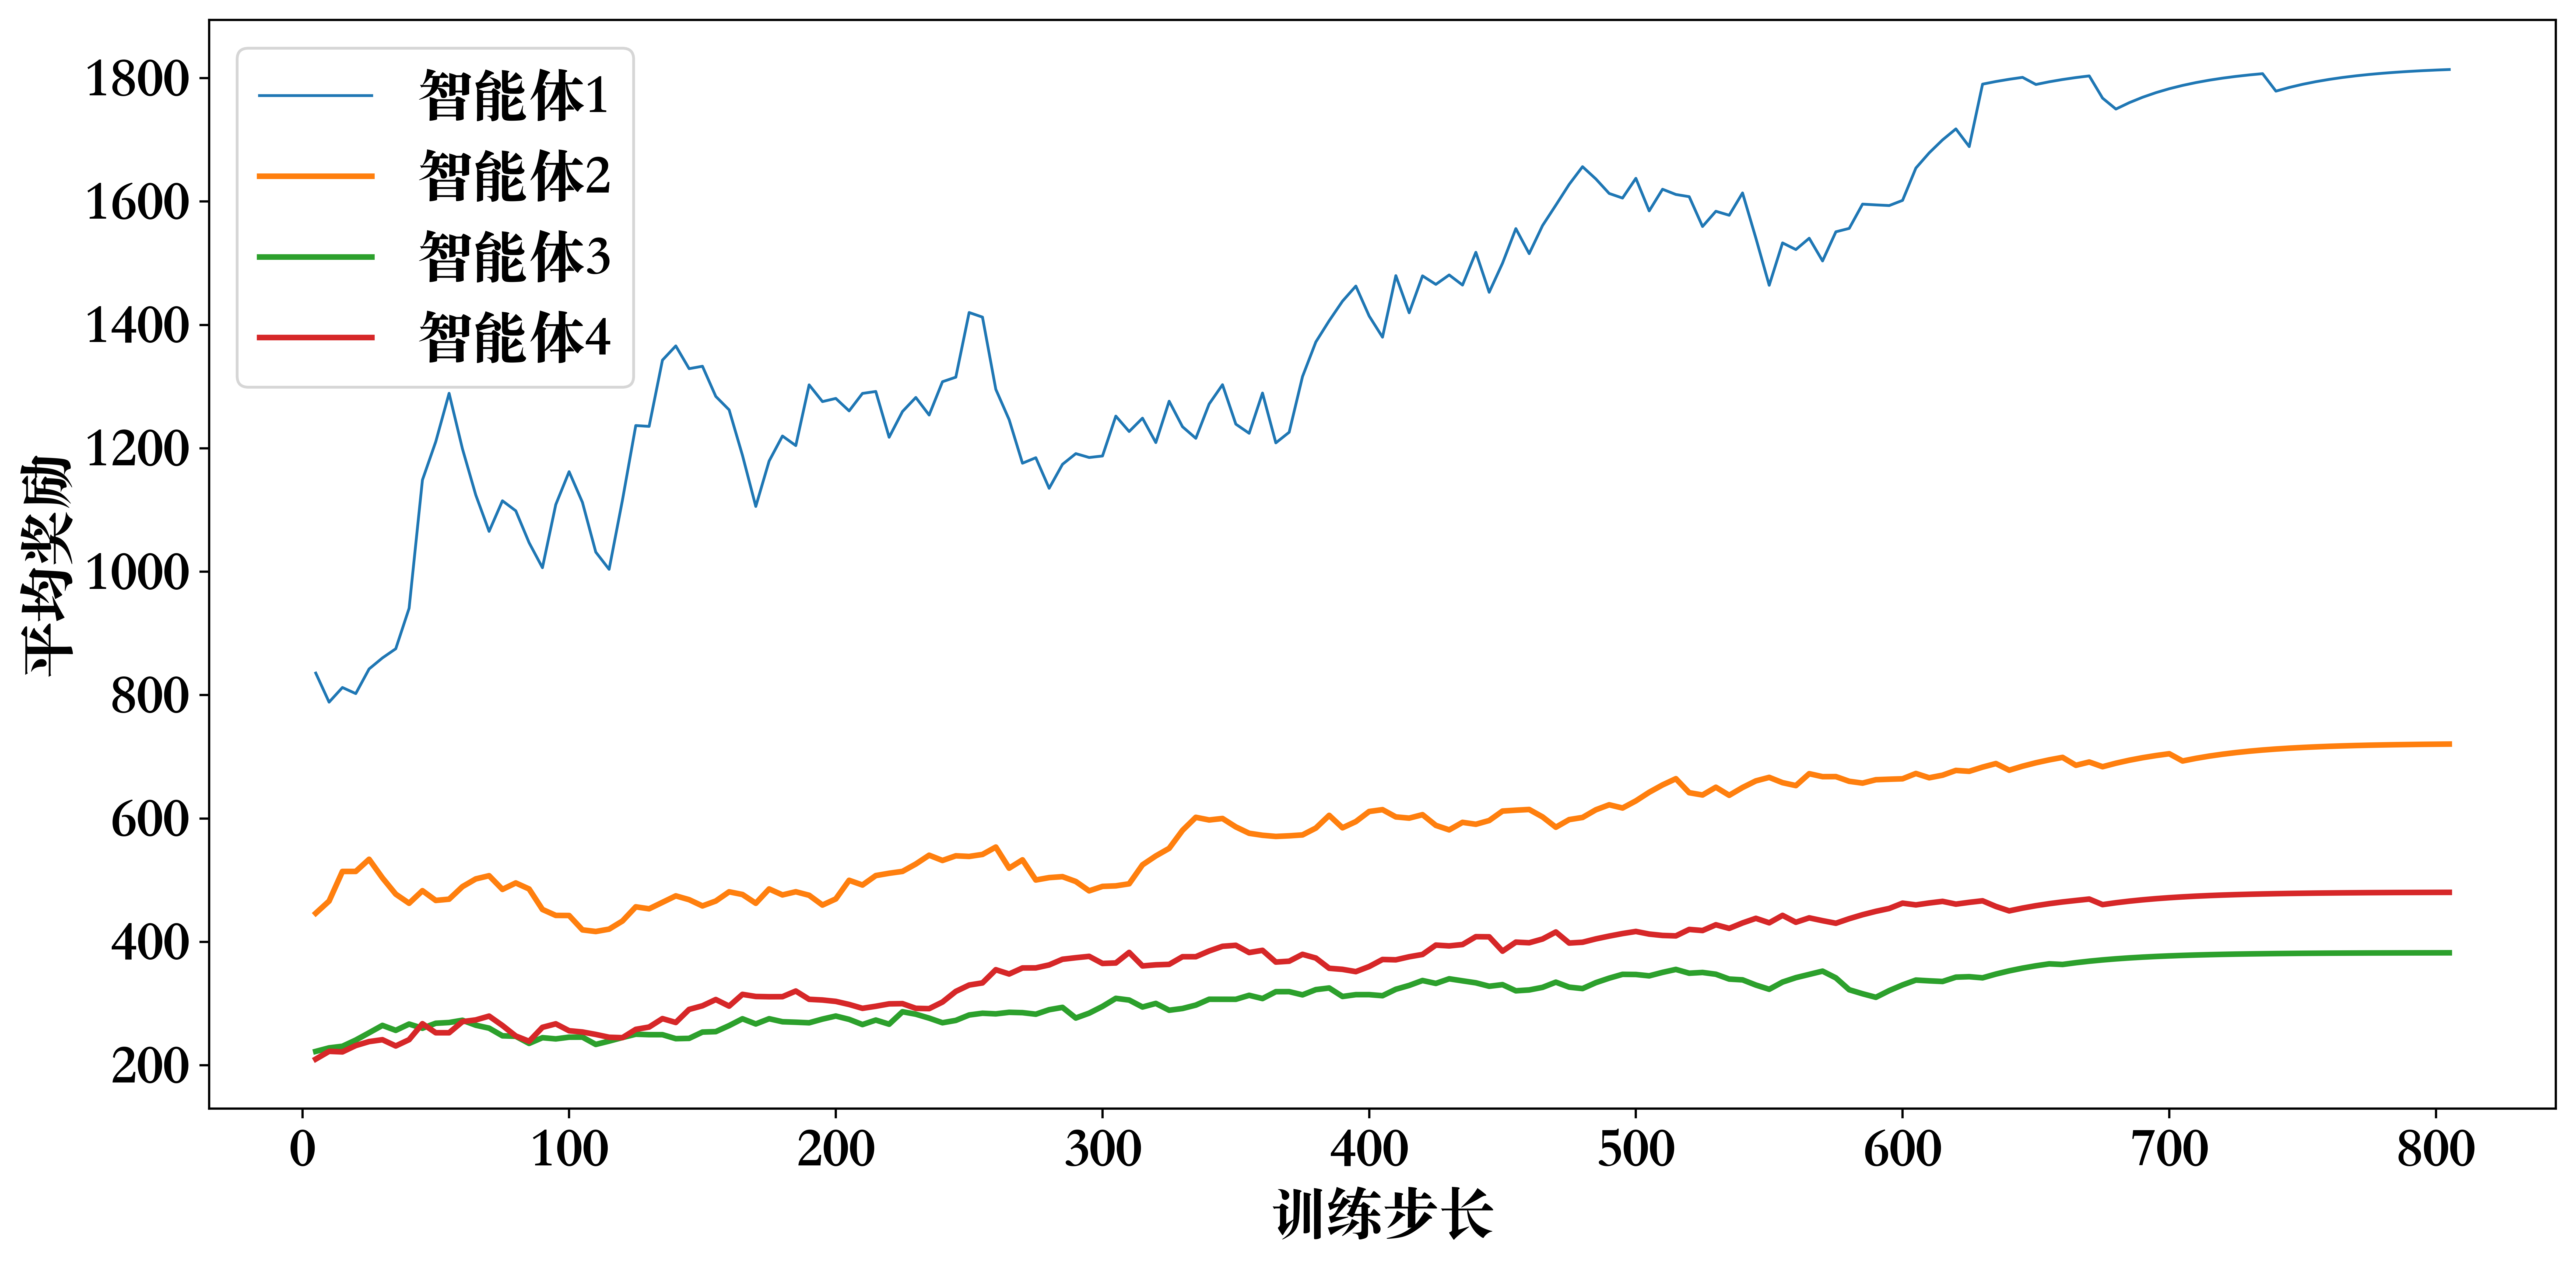
\includegraphics[width=.85\textwidth]{figures/content/reward.png}}
  \label{reward}
  \caption{训练过程中各个代表智能体损失值与奖励值的变化图像}
  \label{loss&reward}
\end{figure}

图\ref{agents}中展示了四个代表性个体在训练过程中遵循的深度强化学习建议行动。初始阶段,智能体的行动变化频繁,这是由于行动探索阶段所导致的。在这个阶段,智能体个体主要通过不断地尝试来了解环境并寻找最佳策略。由于环境的不确定性,智能体可能会尝试多种不同的行动,以了解每种行动的结果和潜在收益。但是,一旦智能体个体进入利用阶段,它们开始依赖其已经学习到的知识和经验,从而选择能够带来最大收益的行动。在这个阶段,由于智能体个体已经建立了一个比较准确的环境模型和策略,所以行动变化的波动性逐渐减小,每个智能体个体似乎已经找到了其自身出行模式与出发时间的最优解。在利用阶段期间,智能体个体偶尔会进行一些行动更改,这可能是由于$\varepsilon$-贪心策略所导致的。$\varepsilon$-贪心策略是一种在训练初期使用的策略,其目的是在探索阶段时增加行动的随机性,从而帮助智能体个体更好地了解环境。随着训练的进行,$\varepsilon$的值逐渐降低到一个非常小的值,从而逐渐减小了随机性,使得智能体个体的行动更加稳定和准确。总的来说,这些观察结果表明,深度强化学习算法在训练过程中,智能体个体通过探索与利用阶段的交替学习,最终学会了最优策略,并且能够在不同的情况下做出正确的决策。


\begin{figure}[htbp]
  \subfloat[智能体1]{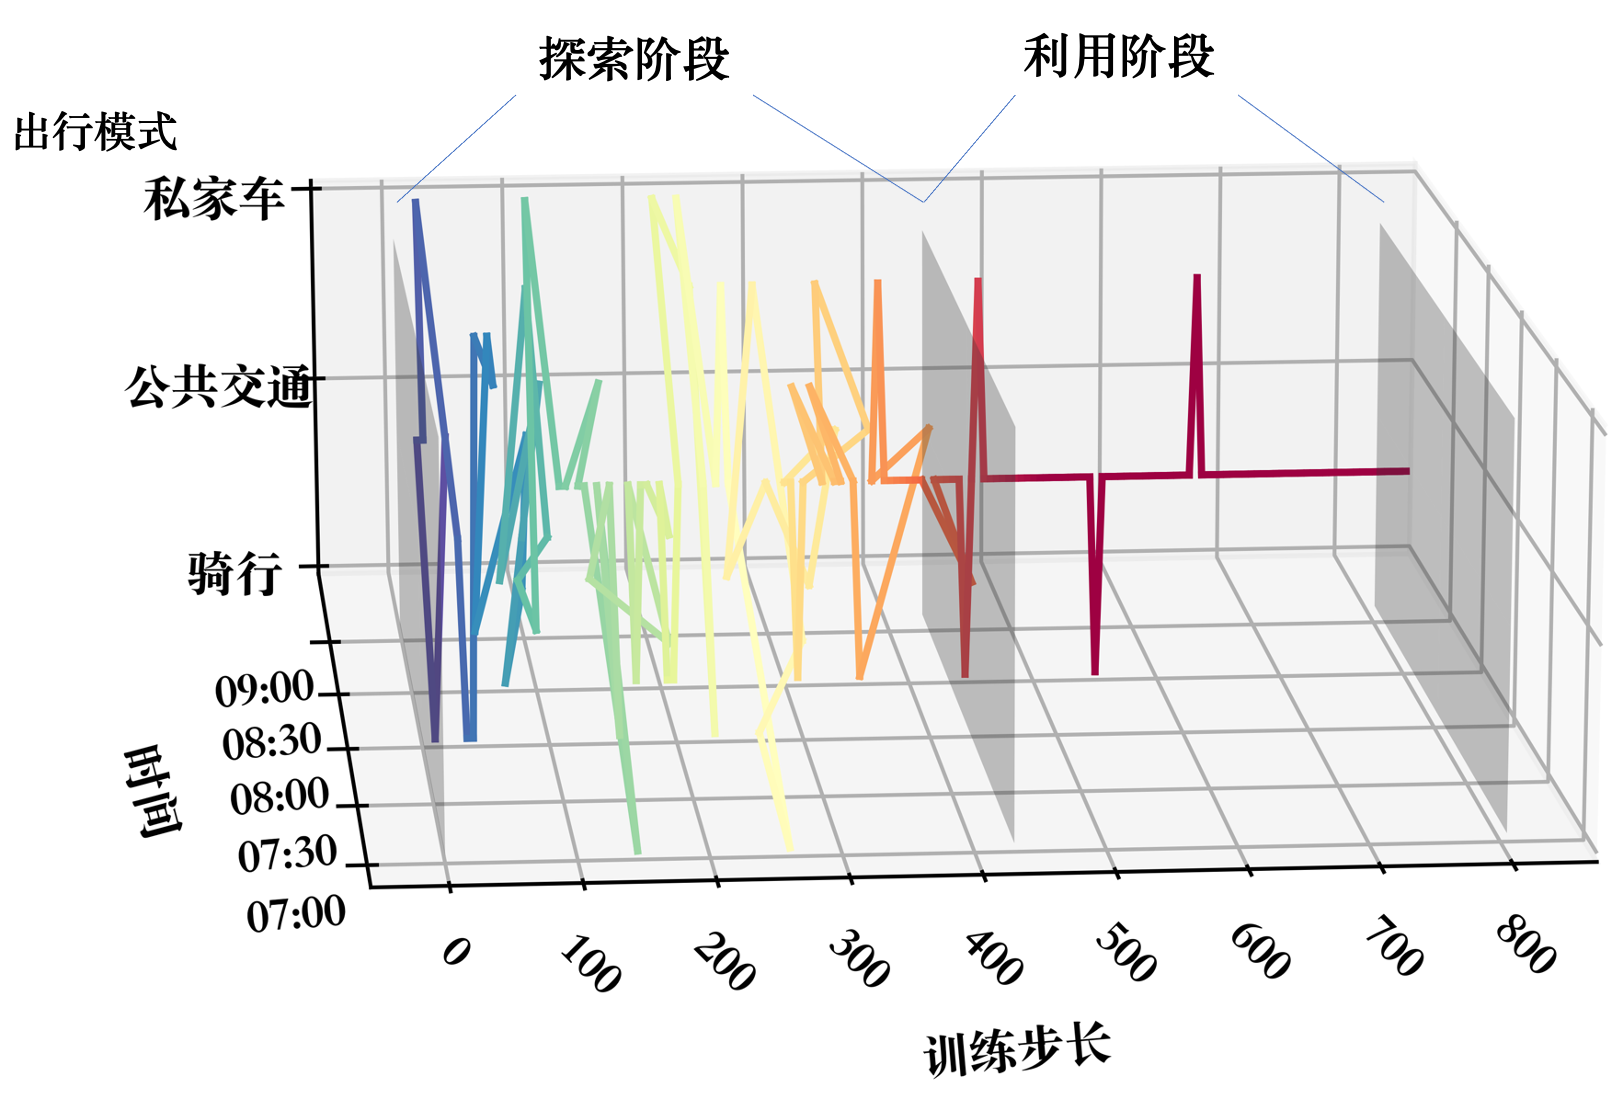
\includegraphics[width=.5\textwidth]{figures/content/action1.png}}
  \quad\quad
  \subfloat[智能体2]{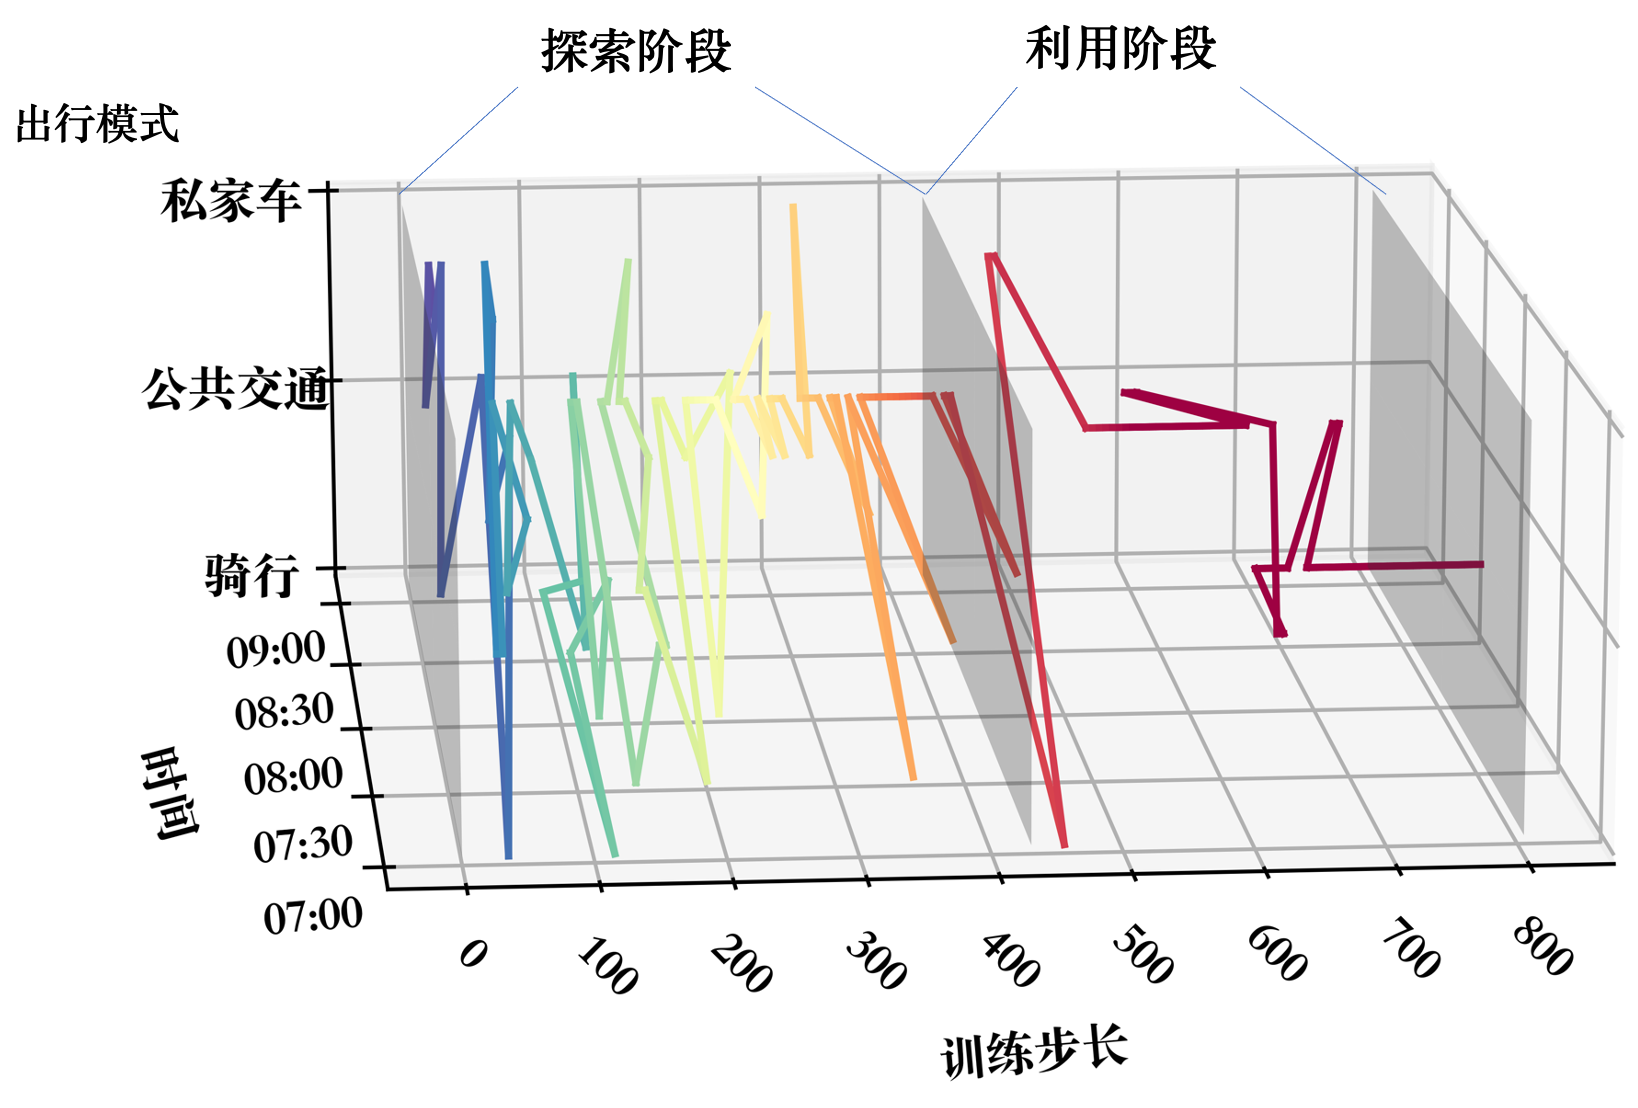
\includegraphics[width=.5\textwidth]{figures/content/action2.png}}
  \\
  \subfloat[智能体3]{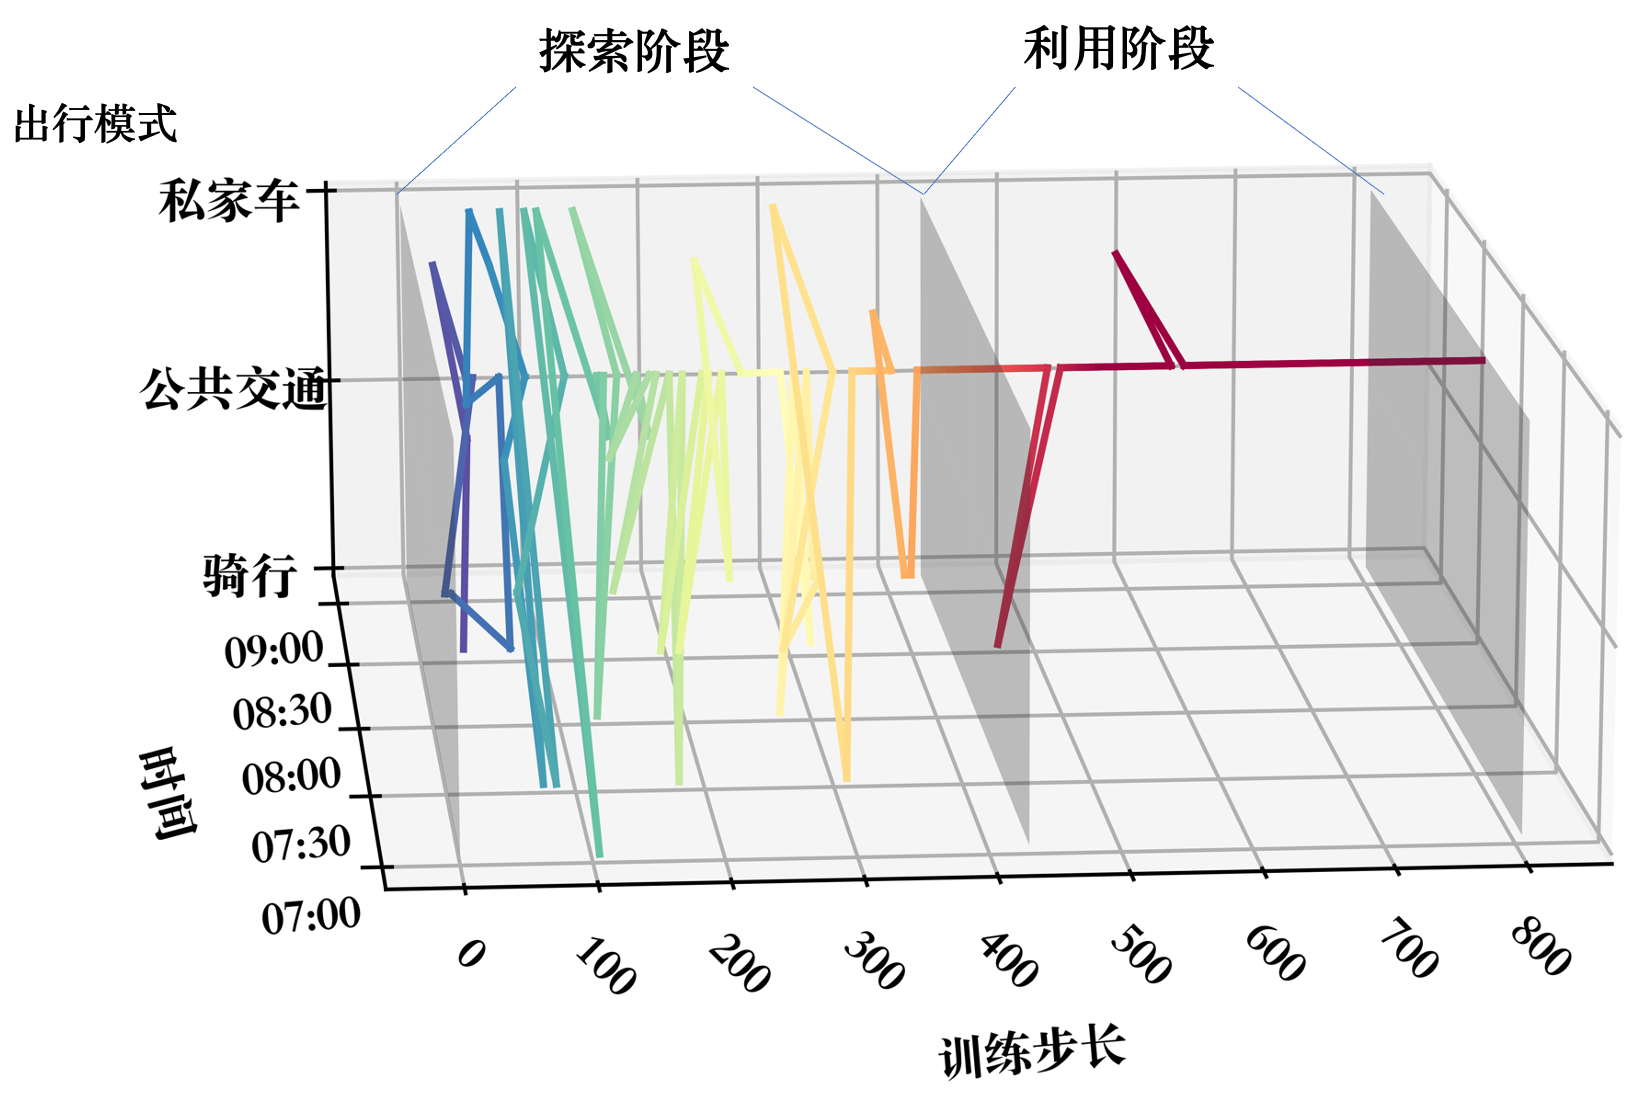
\includegraphics[width=.5\textwidth]{figures/content/action3.png}}
  \quad\quad
  \subfloat[智能体4]{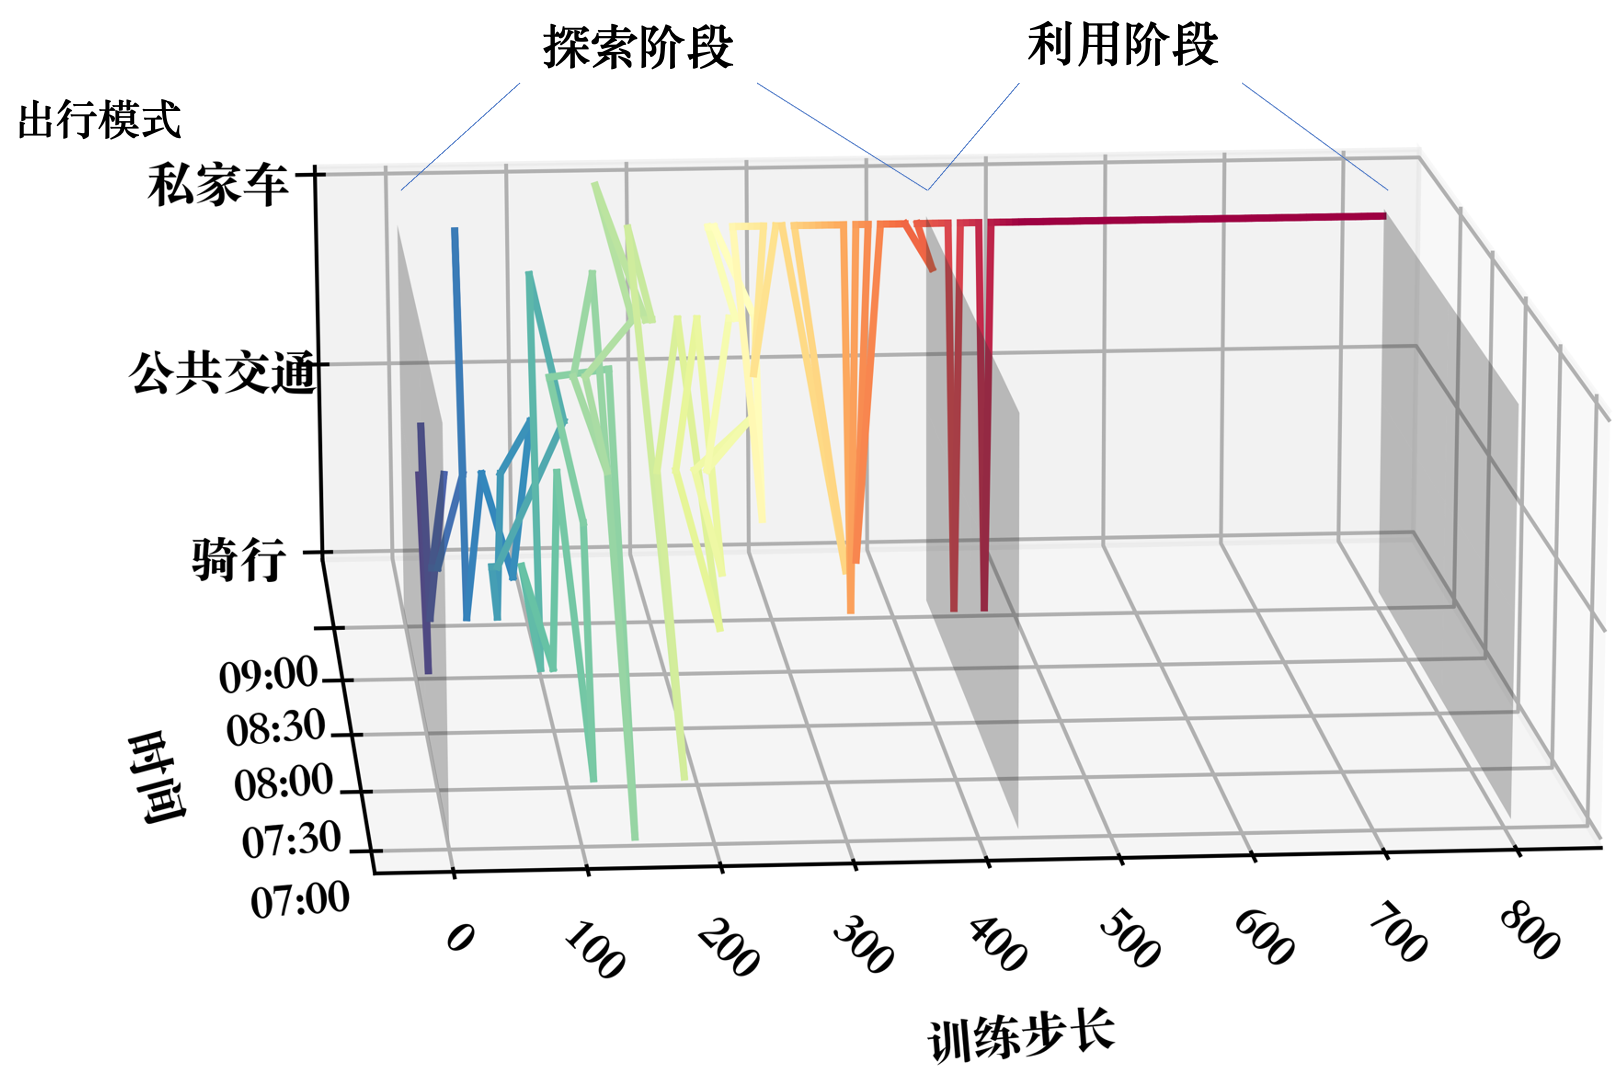
\includegraphics[width=.5\textwidth]{figures/content/action4.png}}
  \caption{训练过程中代表智能体的动作选择变化}
  \label{agents}
\end{figure}




\section{模型的评估}

在本节中,将对基于深度强化学习的出行模式与时间选择模型进行评估,其目的在于验证模型的有效性和泛化能力。本节将分别从模型泛化能力检验、与传统方法的对比和模型参数的灵敏度分析三个方面对模型进行评估。在泛化能力检验中,使用测试集对模型进行测试,以验证其在不同数据集上的表现;在对比传统方法方面,将使用传统的离散选择方法与深度强化学习方法进行对比,并分析两者的优劣势;最后,在参数灵敏度分析中,将探讨模型参数对模型表现的影响,以确定模型最优参数。

\subsection{模型泛化能力检验}

为了对模型的泛化能力进行了测试,从训练数据中随机选取一部分个体,并将其作为测试集。然后对这些测试集中的个体进行测试,并计算其平均奖励值。为了检验所提出方法得到的解决方案的优劣或最优性,将所提出的方法与传统DQN方法和朴素法进行比较。传统DQN方法是一种已经被广泛研究和应用的深度强化学习方法,因此可以作为一个有代表性的基准。而朴素法是一种简单的贪心算法,它的性能不如传统DQN和所提出的方法,但它的计算复杂度很低,因此可以作为一种基准来比较所提出方法的性能。通过与传统DQN和朴素法的比较,可以验证本文方法的优越性和泛化能力。传统DQN方法与本文方法不同的是将只选择一个智能体样本进行训练。朴素法是在每个仿真中随机选择一个动作,为了充分探索动作空间,朴素法将运行1000个仿真次数。在这次比较分析中,测试数据集选择了网络中50个不同OD的出行个体,这些个体在训练中均没有被考虑。为了进行比较,让每个测试个体根据这些相互比较的决策者之一分别采取行动,并收集所得到的奖励。

图\ref{com}(a)、\ref{com}(b)和\ref{com}(c)展示了三个选定的测试个体的比较结果。结果表明,朴素法的奖励存在显著波动,因为随机选择的行动不能保证总是获得良好的结果。相比之下,所提出方法和普通DQN获得的奖励是与JTMDTC问题的最优解相关的单一值,如图中的直线所示。在这三个测试个体中,所提出方法给出的解决方案优于普通DQN,更优于大部分朴素法给出的解决方案,这一结果明显可见于图\ref{com}(a)和\ref{com}(c)。

为了更全面地了解所有50个测试个体的比较情况,找到了朴素法为每个测试个体获得的最大奖励,将其视为该个体出行模式和出发时间问题的近似最优解。将所提出方法和传统DQN给出的解决方案与这个参考值进行比较,可以从全局角度观察性能差异。图\ref{com}(d)显示,本文方法的大部分解决方案(超过40个)超过了参考奖励值的95\%,这意味着这些解决方案接近最优。然而,对于普通的DQN来说,情况并非如此。只有大约30\%的解决方案超过了同一参考值的95\%,还有相当多的解决方案甚至低于参考值的60\%。这些比较结果表明,所提出的方法在解决许多个体的出行模式和出发时间问题时具有有效性,并且代表在完成这个任务中所发挥的重要作用。由于测试个体并不是训练的一部分,结果表明所提出方法具有良好的可迁移性。

\begin{figure}[htbp]
  \subfloat[智能体1]{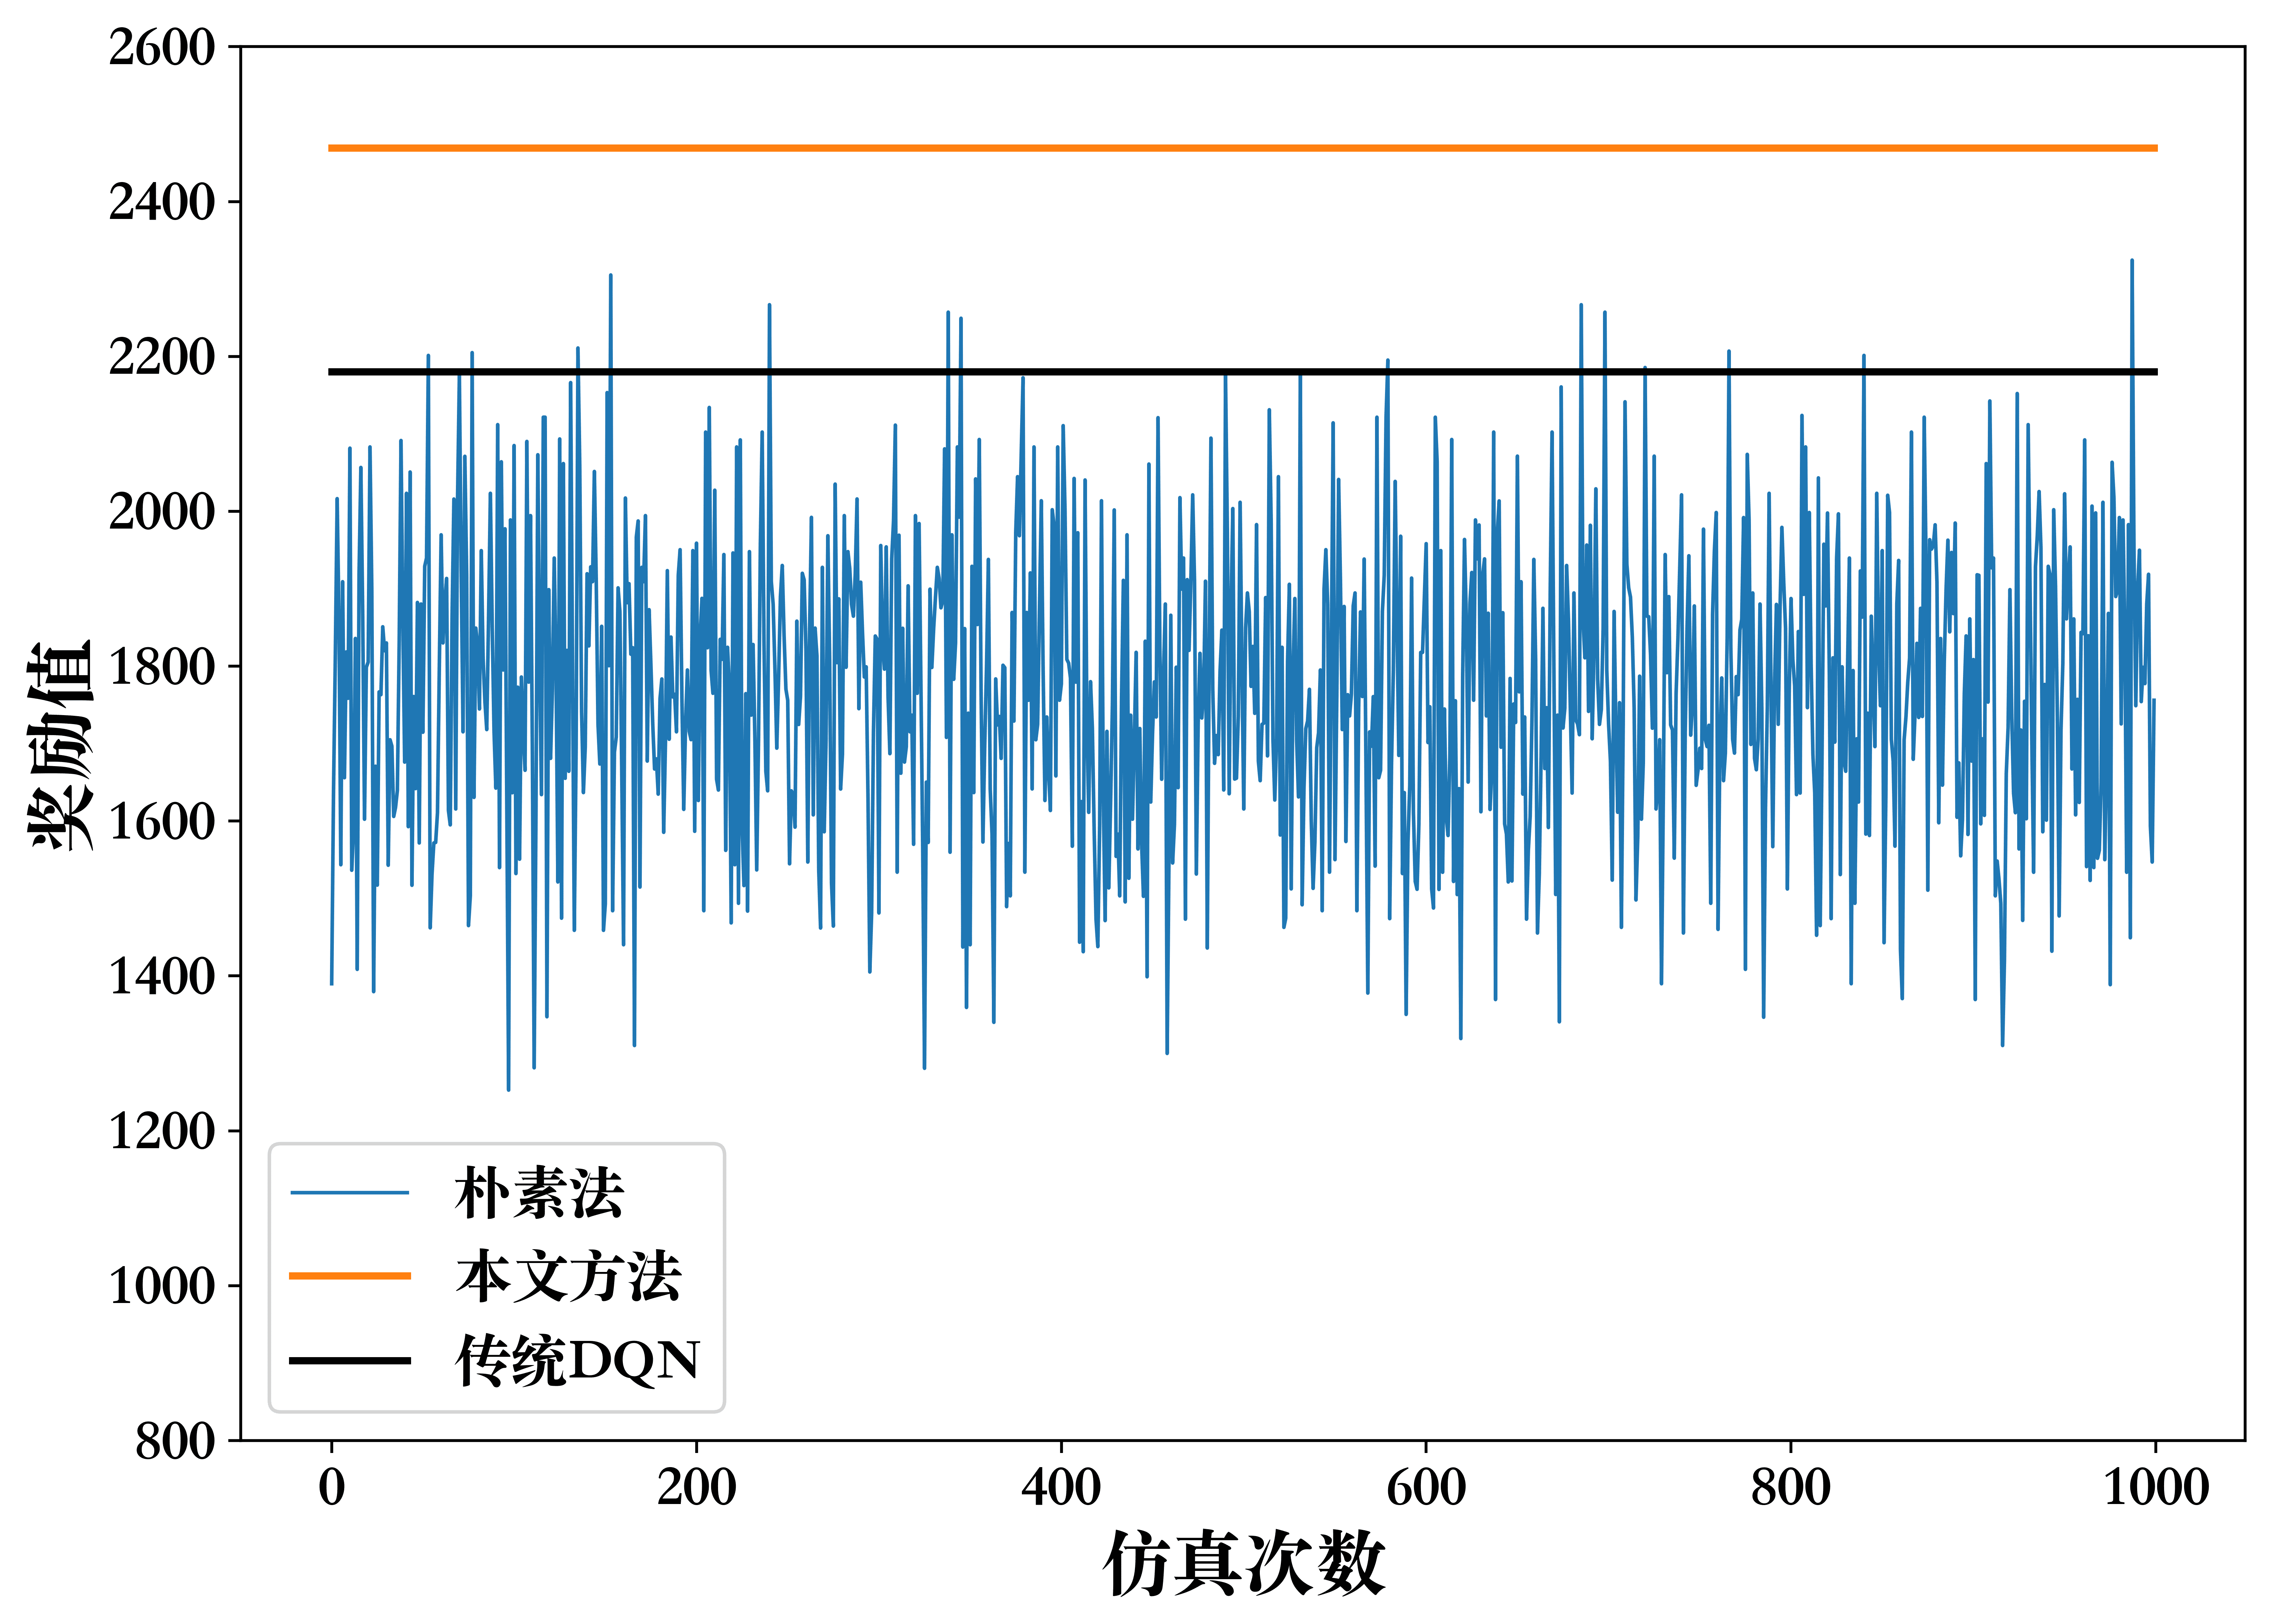
\includegraphics[width=.5\textwidth]{figures/content/com1.png}}
  \quad\quad
  \subfloat[智能体2]{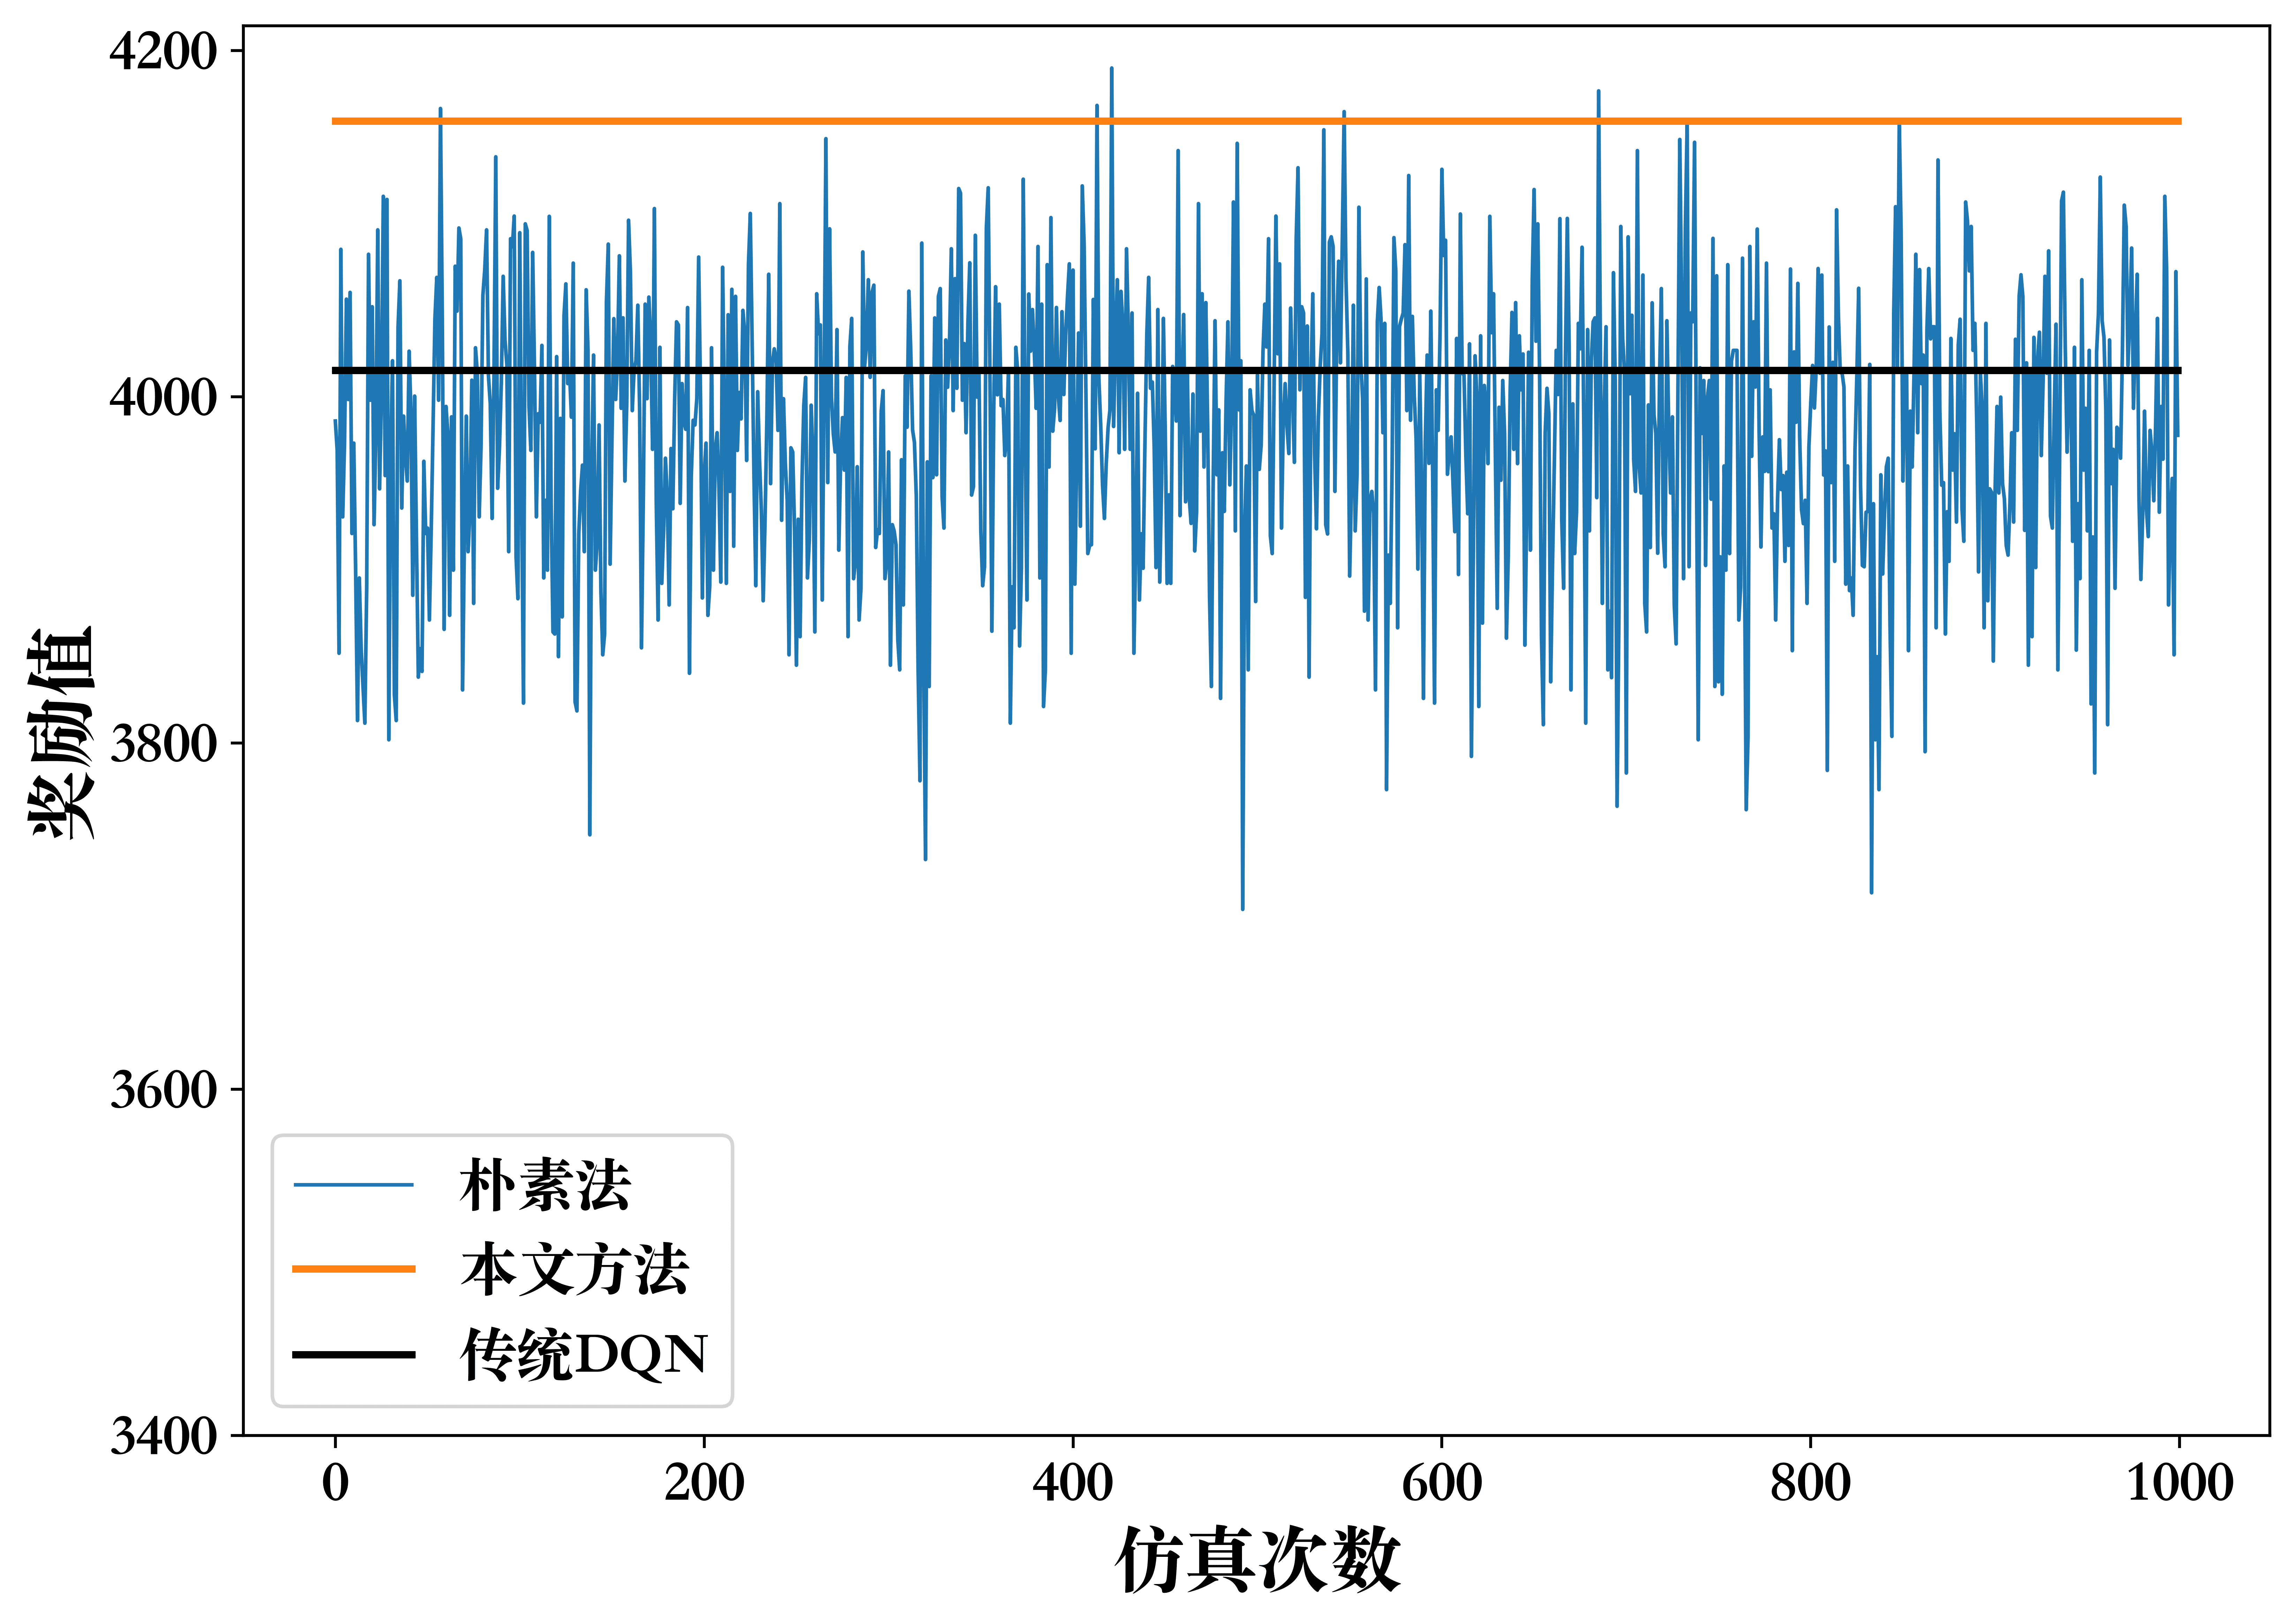
\includegraphics[width=.5\textwidth]{figures/content/com2.png}}
  \\
  \subfloat[智能体3]{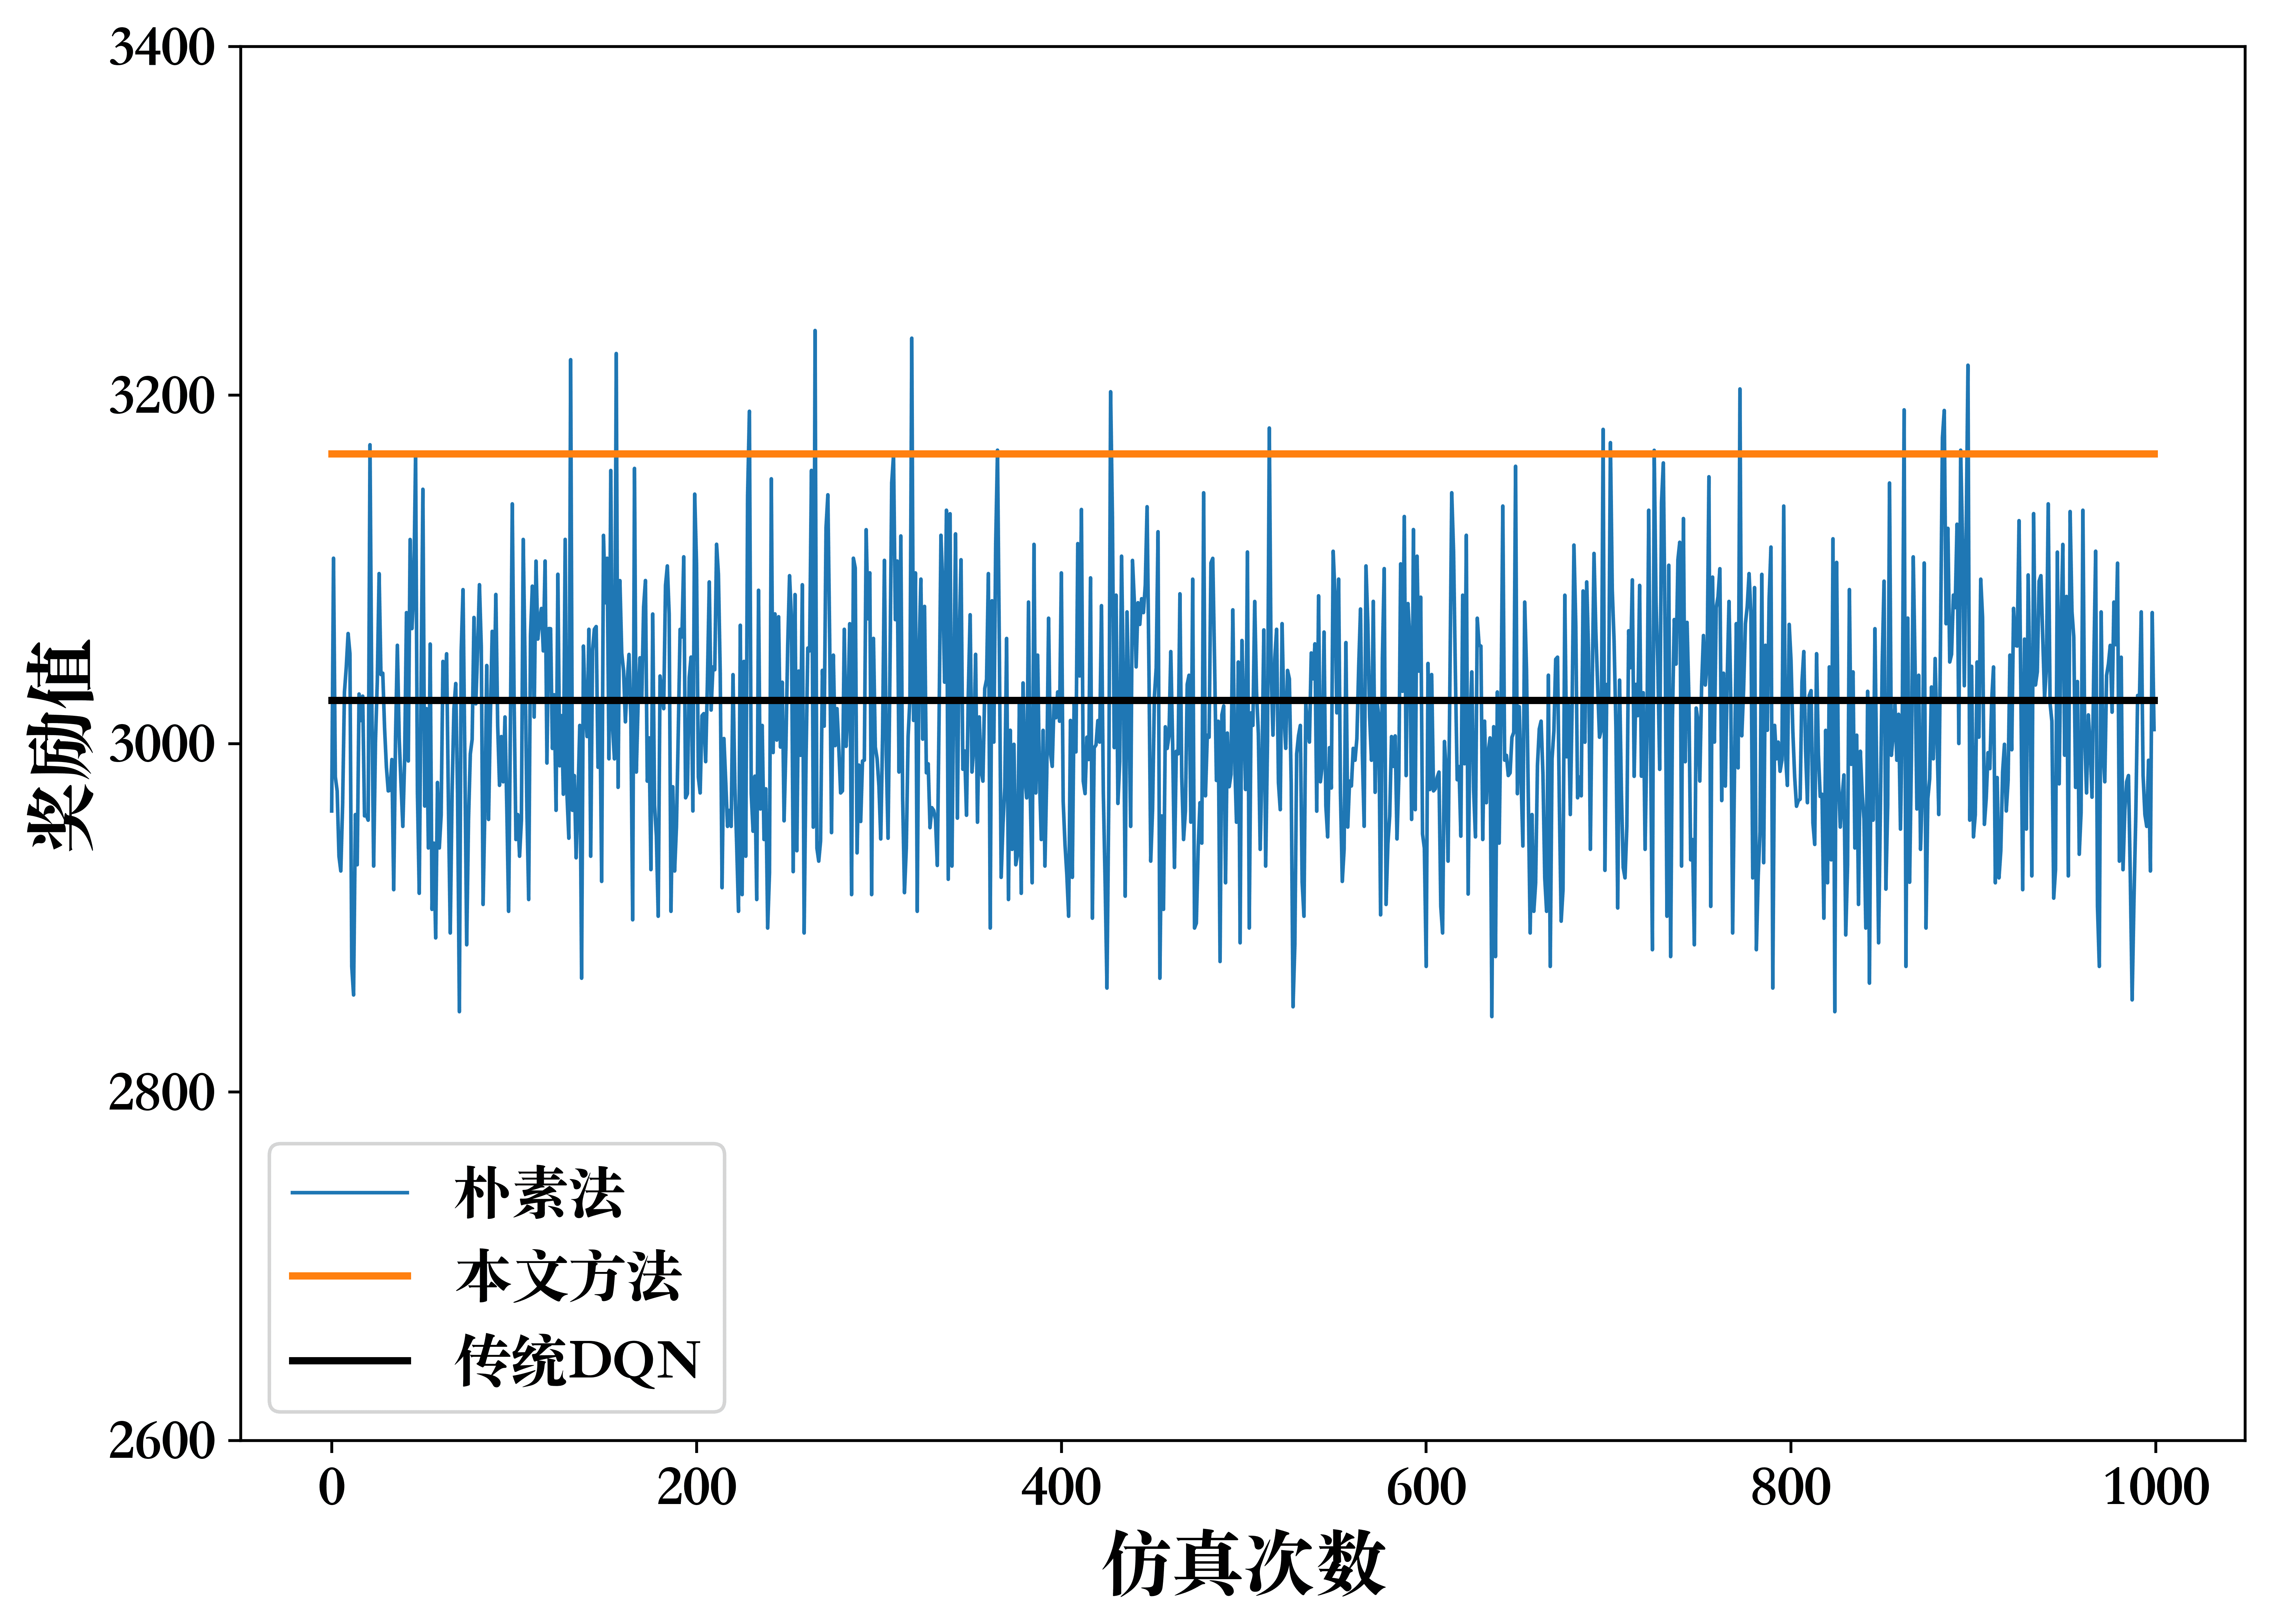
\includegraphics[width=.5\textwidth]{figures/content/com3.png}}
  \quad\quad
  \subfloat[智能体4]{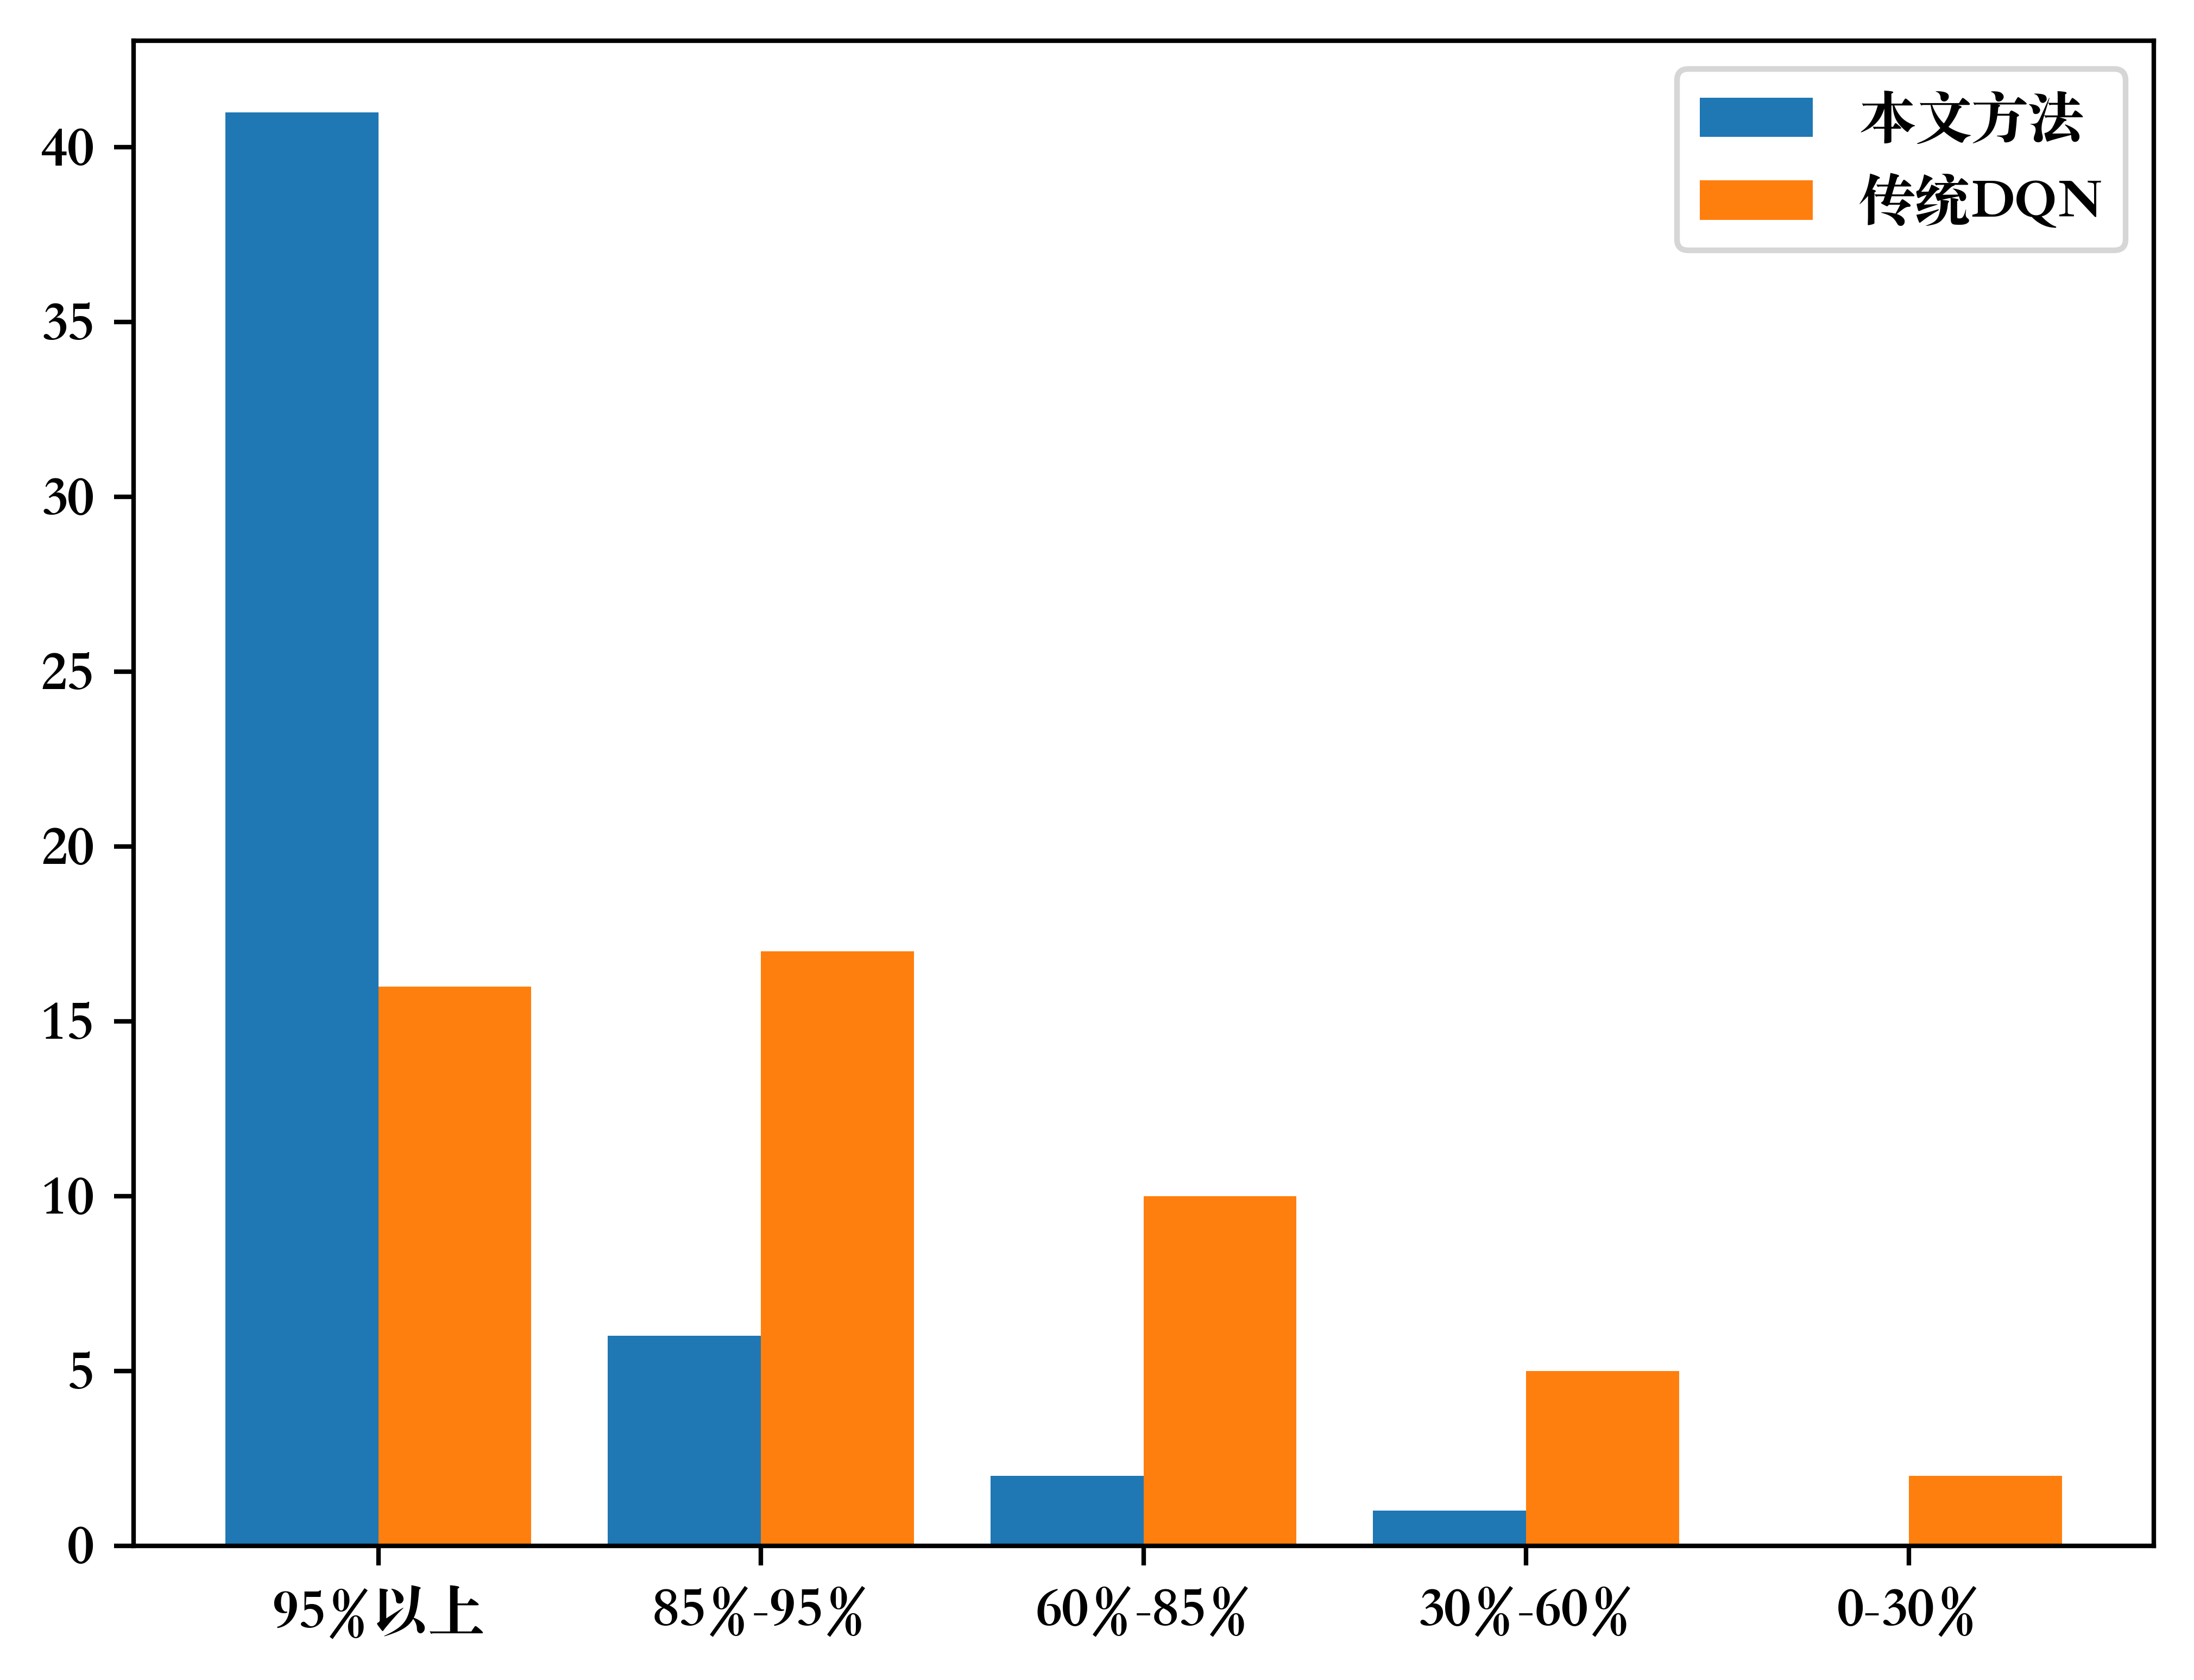
\includegraphics[width=.5\textwidth]{figures/content/com4.png}}
  \caption{训练过程中代表智能体的动作选择变化}
  \label{com}
\end{figure}

在本次实验中,随机选取了一部分个体,并将其用作测试集。然后,对这些测试集中的个体进行了测试,并计算了它们的平均奖励值。结果表明,测试集中的个体的表现略低于训练集中的个体,但仍表现出较好的性能。这表明所提出的方法具有一定的泛化能力,即能够适应一些新的情况并产生有意义的结果。


\subsection{部分信息的模型检验}

在现实世界中,人们在做出决策时,通常不会拥有完全的信息,例如,可能无法准确地了解周围环境、其他人的行为、交通状况等。因此,仅仅依靠部分信息进行决策,可能会导致更差的行动选择。为了比较所提出的深度强化学习方法的性能,此小节引入了另外两种模型,以考虑在部分信息的情况下,深度强化学习方法是否仍然是有效的。

第一个是一阶马尔可夫链(MC)模型,仅使用当前旅行距离和出发时间差来决定下一个选择。其状态、转移和初始状态概率以及奖励函数均源自DRL模型。两者的主要区别在于决策过程。MC模型使用转移和初始状态概率来模拟随时间变化的行为,而深度强化学习模型使用迭代试错过程。在一阶马尔可夫链(MC)模型中,每个时间步都可以看作是一个状态,用$s_t$表示。模型假设,行为只取决于当前状态$s_t$,并且在状态$s_t$下,采取行动$a_t$会以概率$p(s_{t+1}|s_t, a_t)$转移到下一个状态$s_{t+1}$,其中$p(s_{t+1}|s_t, a_t)$表示在状态$s_t$下采取行动$a_t$并转移到状态$s_{t+1}$的概率。这个概率可以通过训练数据中的频率来估计。另外,MC模型还需要一个初始状态分布$\mu$,表示在开始时每个状态的出现概率。这个分布也可以通过训练数据中的频率来估计。在决策过程中,MC模型首先从初始状态分布$\mu$中随机选取一个初始状态$s_0$。然后,在每个时间步$t$,根据当前状态$s_t$和行动$a_t$,使用转移概率$p(s_{t+1}|s_t, a_t)$随机转移到下一个状态$s_{t+1}$。在每个时间步,根据当前状态$s_t$和一些其他信息(例如旅行时间,距离等),MC模型使用某种规则(例如贪心算法)选择下一个行动$a_t$,直到终止状态被达到。相比之下,深度强化学习方法不仅使用状态和行动,还使用神经网络来学习状态和行动之间的复杂映射关系,并使用Q值函数来指导行动选择。因此,深度强化学习方法具有更好的表达能力和泛化能力,可以更好地处理具有大量状态和行动的环境。

第二个是传统的MNL模型,传统的MNL模型是基于多项式逻辑回归的经典模型,它用于预测个体选择某个行动的概率。MNL模型通常使用可解释的特征来描述选择行动的动机。这些特征通常是人为选择的,而不是通过学习过程得到的。例如,特征可能包括行动的属性(如价格、距离、时间等),个体的属性(如性别、年龄、收入等)等。在本文中,用于对比的MNL模型使用深度强化学习的奖励函数作为效用函数。这里的奖励函数(式(\ref{reward function}))考虑了行动的成本和收益,通过计算收益与成本的比值得到奖励。

使用前文中在信息完全的情况下,由提出的方法得到的个体出行选择作为基准线,根据其来比较其他模型的性能。考虑了三个性能评估和比较指标。除了奖励值之外,另外两个是负对数损失(NLL)和Jaccard指数。NLL通常用于评估分类任务中的模型性能,特别是在类别不平衡的情况下。在本文中,使用NLL作为评价指标,可以测量每种模型的预测能力,即它们在给定历史信息的情况下是否能够正确地预测个体的行动选择。NLL的较低值表示模型更准确地预测了行动选择,因此较低的NLL值是期望的。Jaccard指数是一种测量相似性的指标。在本文中,它可以测量每个模型产生的行动选择与基准线之间的相似程度。基准线是在信息完全的情况下,由提出的方法得到的个体出行选择。因此,Jaccard指数可以反映其他模型相对于基线的优化水平。值越高表示其他模型的行动选择越接近基线,因此较高的Jaccard指数是期望的。这两个指标都衡量其他模型产生的行动与基线获得的行动之间的接近程度或相似程度。因此,它们可以反映其他模型相对于基线的优化水平。

表\ref{eva}总结了三个性能指标的比较结果。如预期的那样,在信息完全的情况下,所提出的方法提供了实现尽可能多的奖励的最佳性能。所有其他模型的性能都较差,通过比较平均奖励值就能看出这一点,这些值都低于基线的奖励值。这种趋势也适用于NLL和Jaccard指数。尽管如此,在部分信息的情况下,所提出的方法仍然表现出比一阶MC模型和MNL模型略好的性能,这表明即使存在部分信息,所提出的方法仍然是有效的。

\begin{table}[htbp]
\centering
\caption{不同替代模型的性能评估结果}
\label{tab:eva}
\renewcommand{\arraystretch}{1.2} % 使表格行间距加大1.2倍
\setlength{\tabcolsep}{8mm} % 设置表格列间距为8mm
\small % 设置表格字体大小为小号

\begin{tabular}{lccc}
\toprule
模型 & NLL & 平均回报 & 准确度 \\
\midrule
一阶Markov链模型 & 19.23 & 1,354 & 0.24 \\
离散选择模型 & 24.17 & 1,217 & 0.23 \\
部分信息下的提出方法 & 17.31 & 1,449 & 0.29 \\
完全信息下的提出方法(基线) & \textbackslash{} & 1,735 & \textbackslash{} \\
\bottomrule
\end{tabular}
\end{table}

\subsection{模型参数的灵敏性分析}

我们现在进行两个敏感性分析,以研究所提出方法在模型参数变化时的性能变化。第一个参数是代表数量,第二个参数是训练个体的集合。为了看到前者的影响,我们进行了进一步的实验,分别使用1、10、20和40个代表。我们保持相同的实验设置,将60个个体的时间依赖OD行程聚类成上述数字,以选择训练代表,而其他50个测试个体则用于评估和比较。同样,蛮力方法作为参考。

比较结果总结在表\ref{cluster_size}中。由于内存溢出,40个代表的实验无法在同一台机器上完成,因此没有报告结果。随着代表数量的增加,所需的训练或计算时间增加,这是预期的。然而,代表数量的增加确实会导致更好的奖励。将一个代表转变为四个代表,奖励得到了最大的提高。进一步将该数字增加到10或20并不能显著提高奖励。这个结果表明,增加代表数量不一定划算。实际上,少量代表已经可以在合理的计算时间内产生相当好的结果。使用蛮力方法得到的最大奖励作为参考值,我们比较了所提出的方法所给出的奖励高于参考值95%以上的测试个体数量。如预期的那样,对于4、10和20个代表,这个数字保持较大且变化很小。图6进一步显示了对于不同数量的代表,四个选定测试个体结果的比较。只有一个代表显然不足以击败蛮力方法,而四个或更多代表则产生了有希望的结果。

\begin{figure}[htbp]
  \subfloat[智能体1]{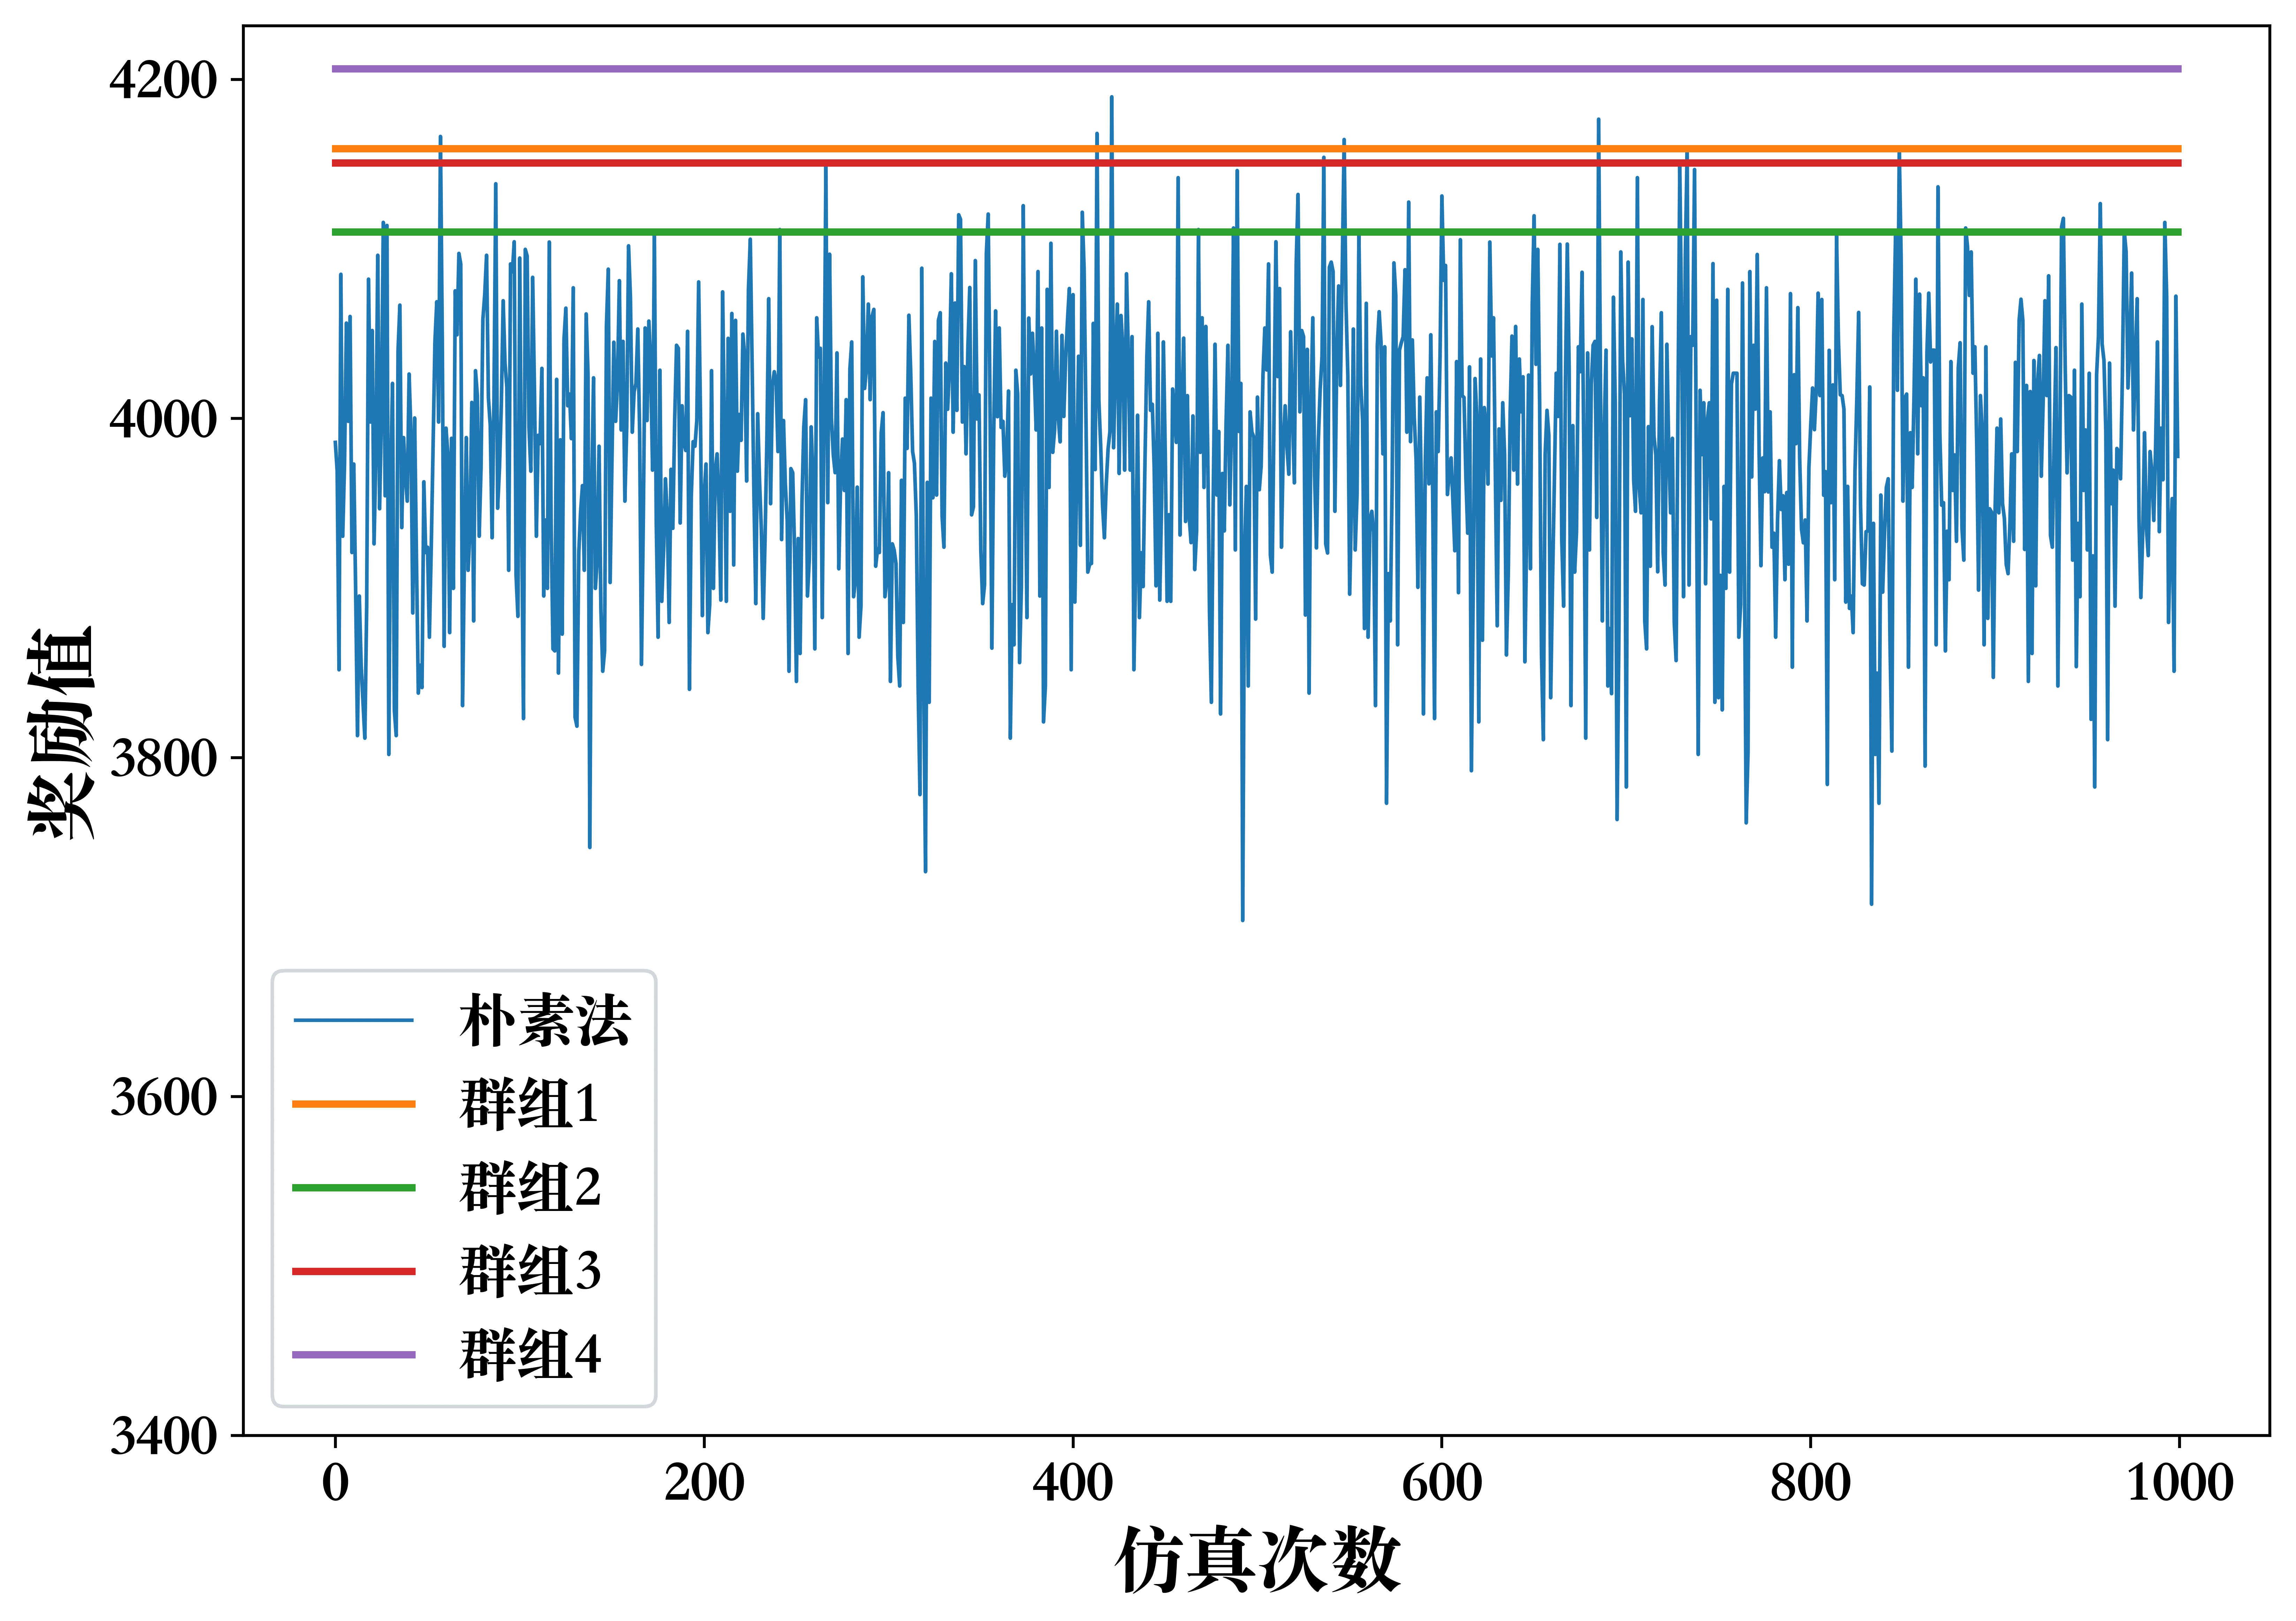
\includegraphics[width=.4\textwidth]{figures/content/agents/agent1.png}}
  \quad\quad
  \subfloat[智能体2]{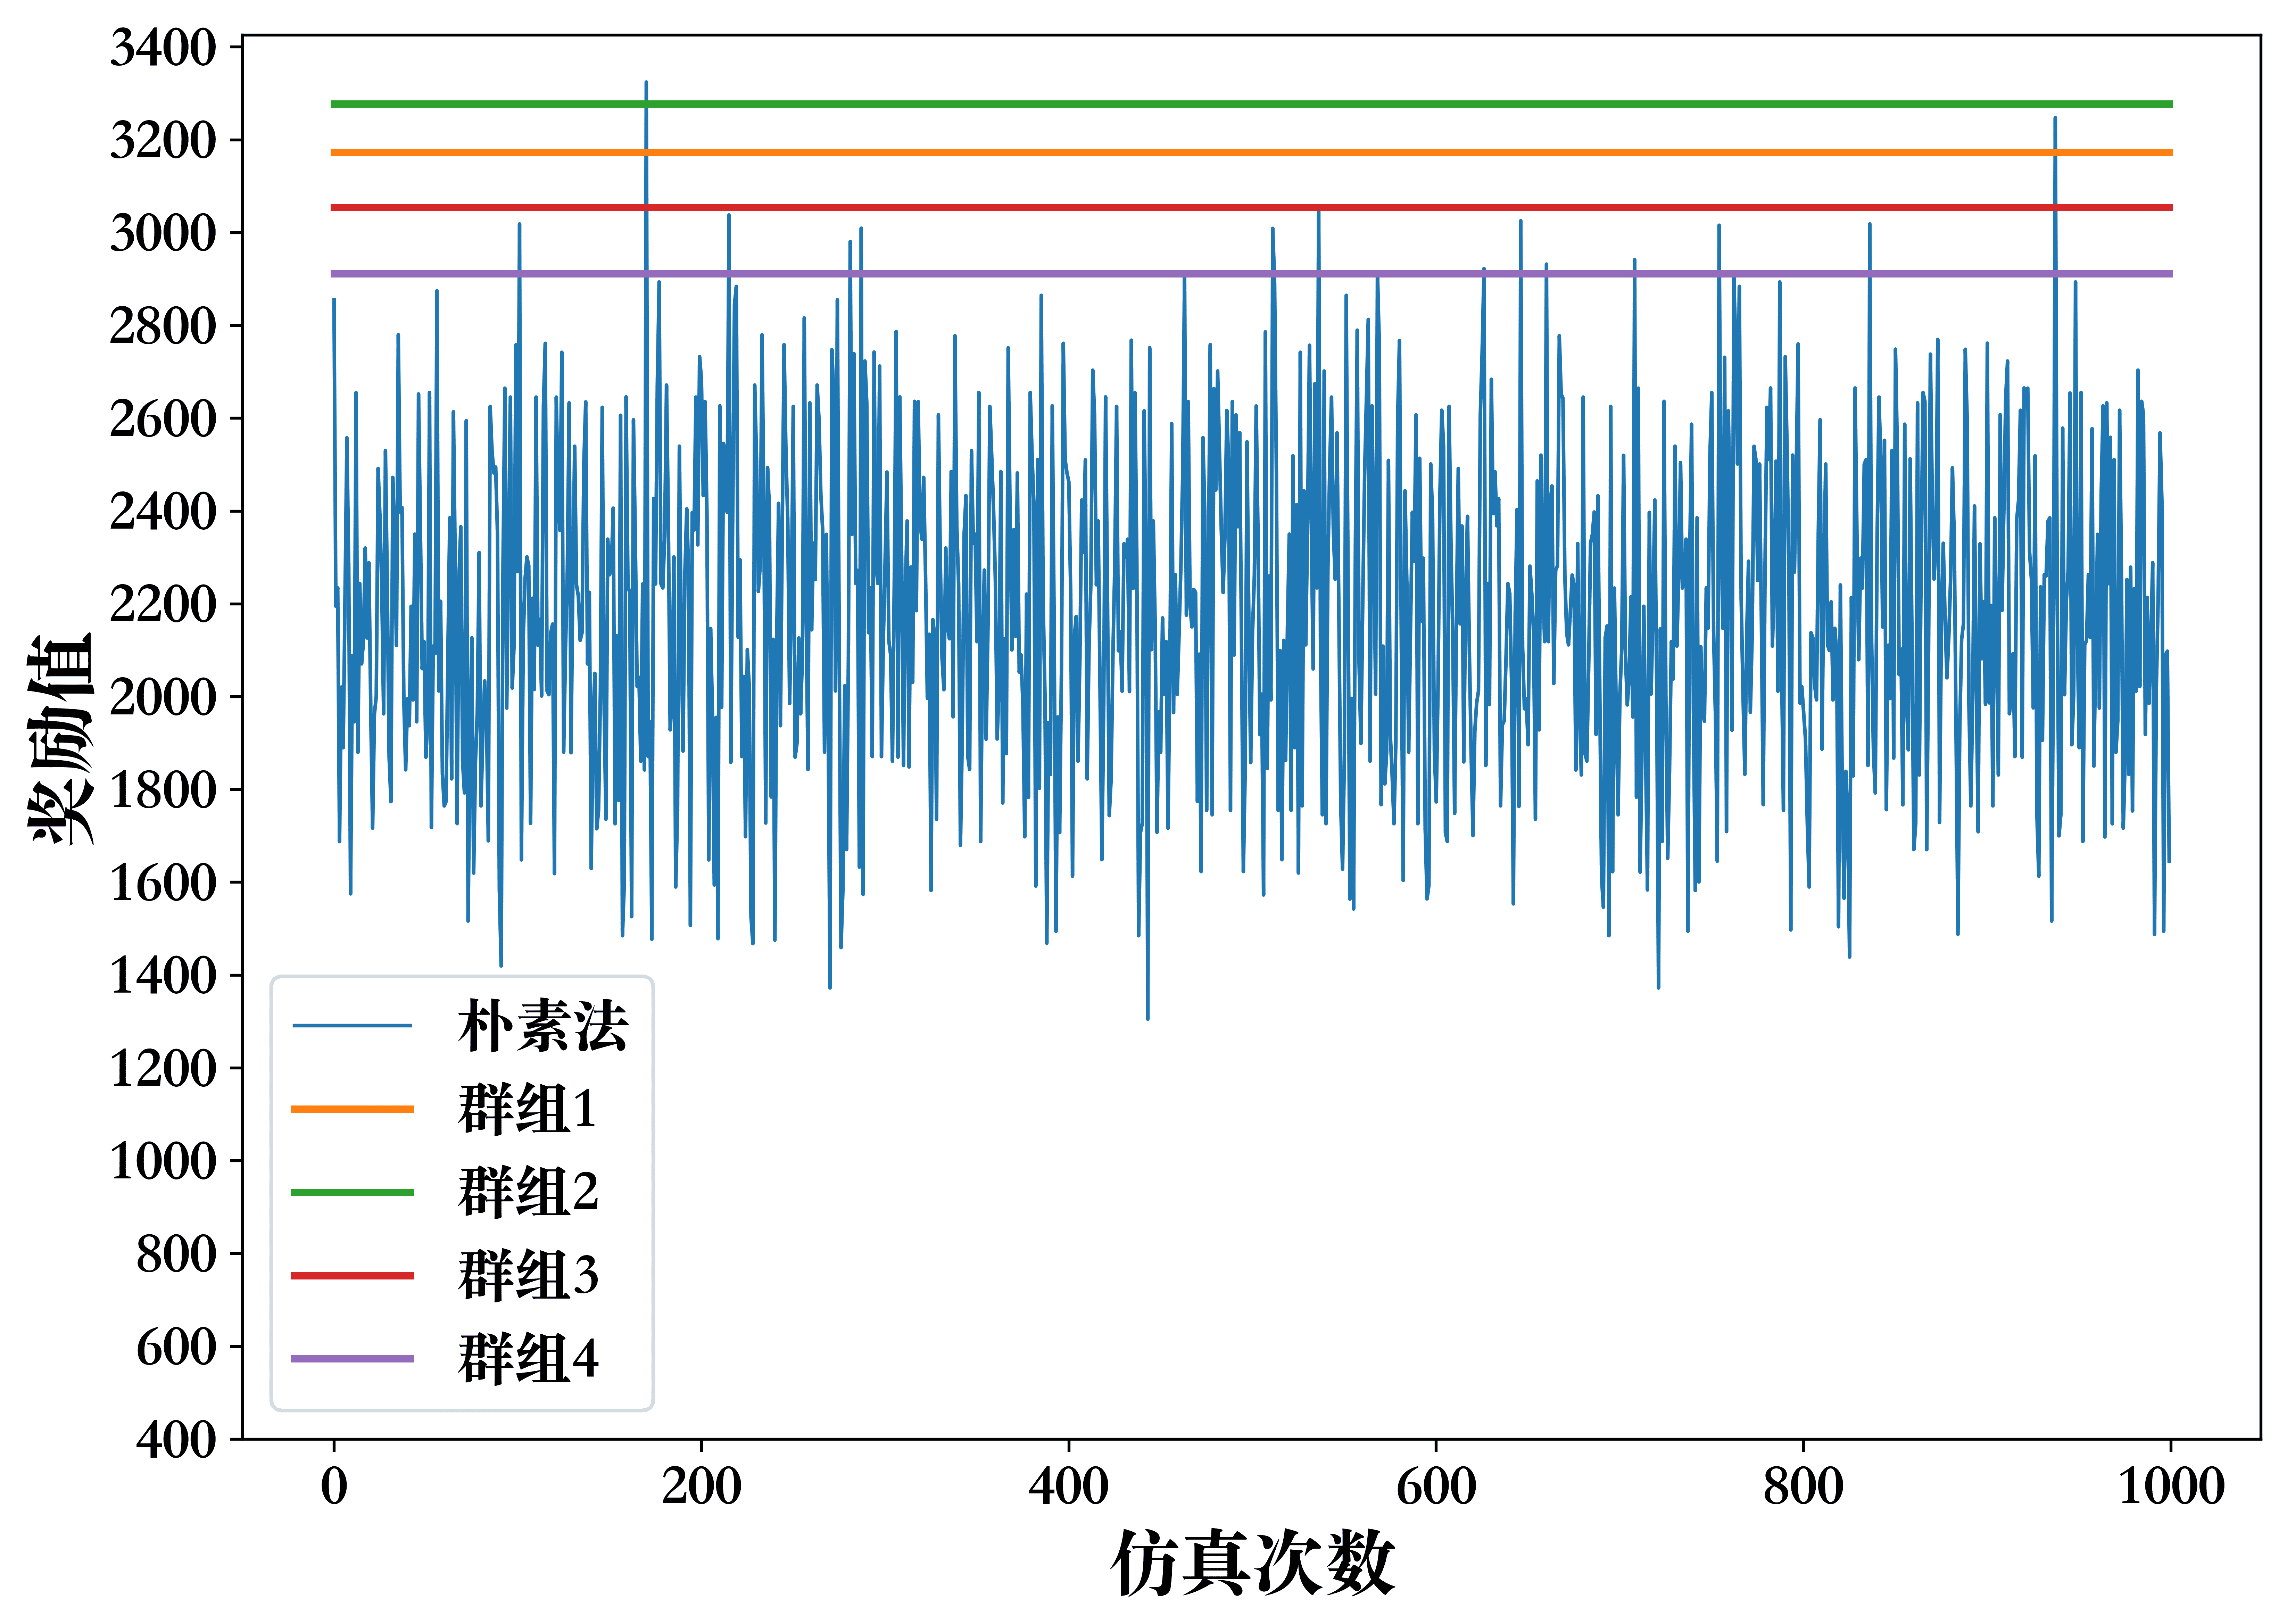
\includegraphics[width=.4\textwidth]{figures/content/agents/agent2.png}}
  \\
  \subfloat[智能体3]{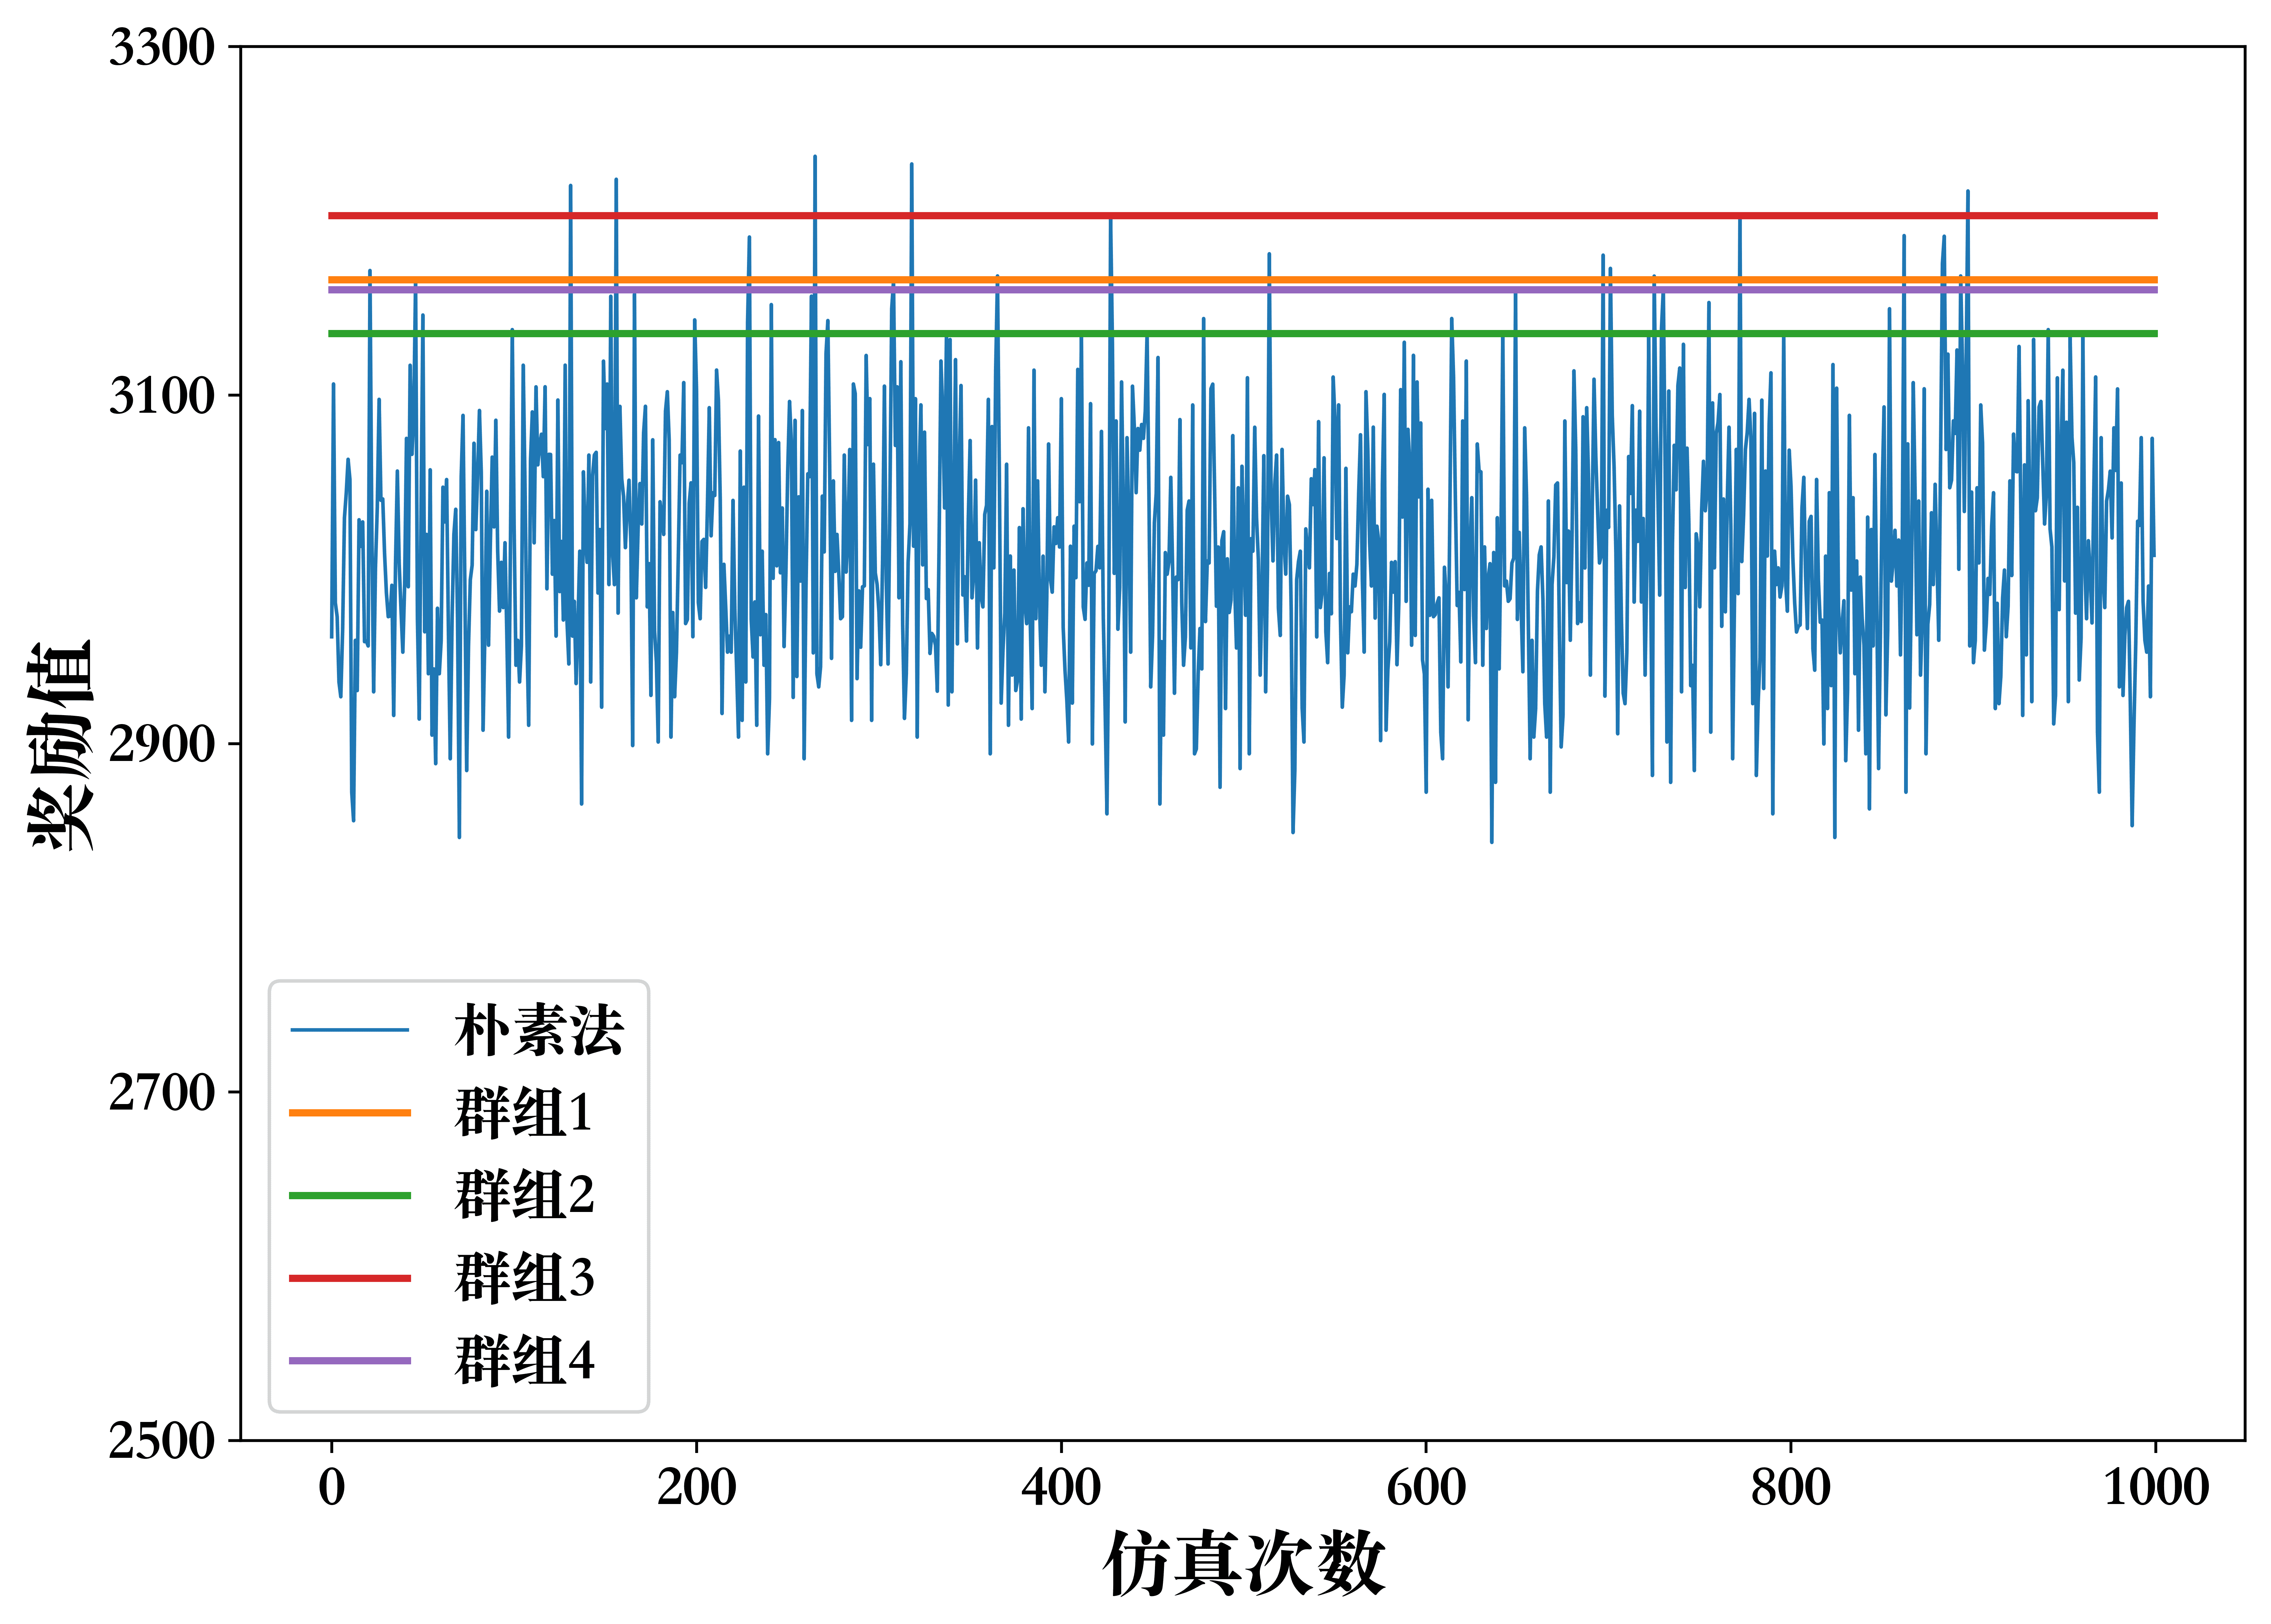
\includegraphics[width=.4\textwidth]{figures/content/agents/agent3.png}}
  \quad\quad
  \subfloat[智能体4]{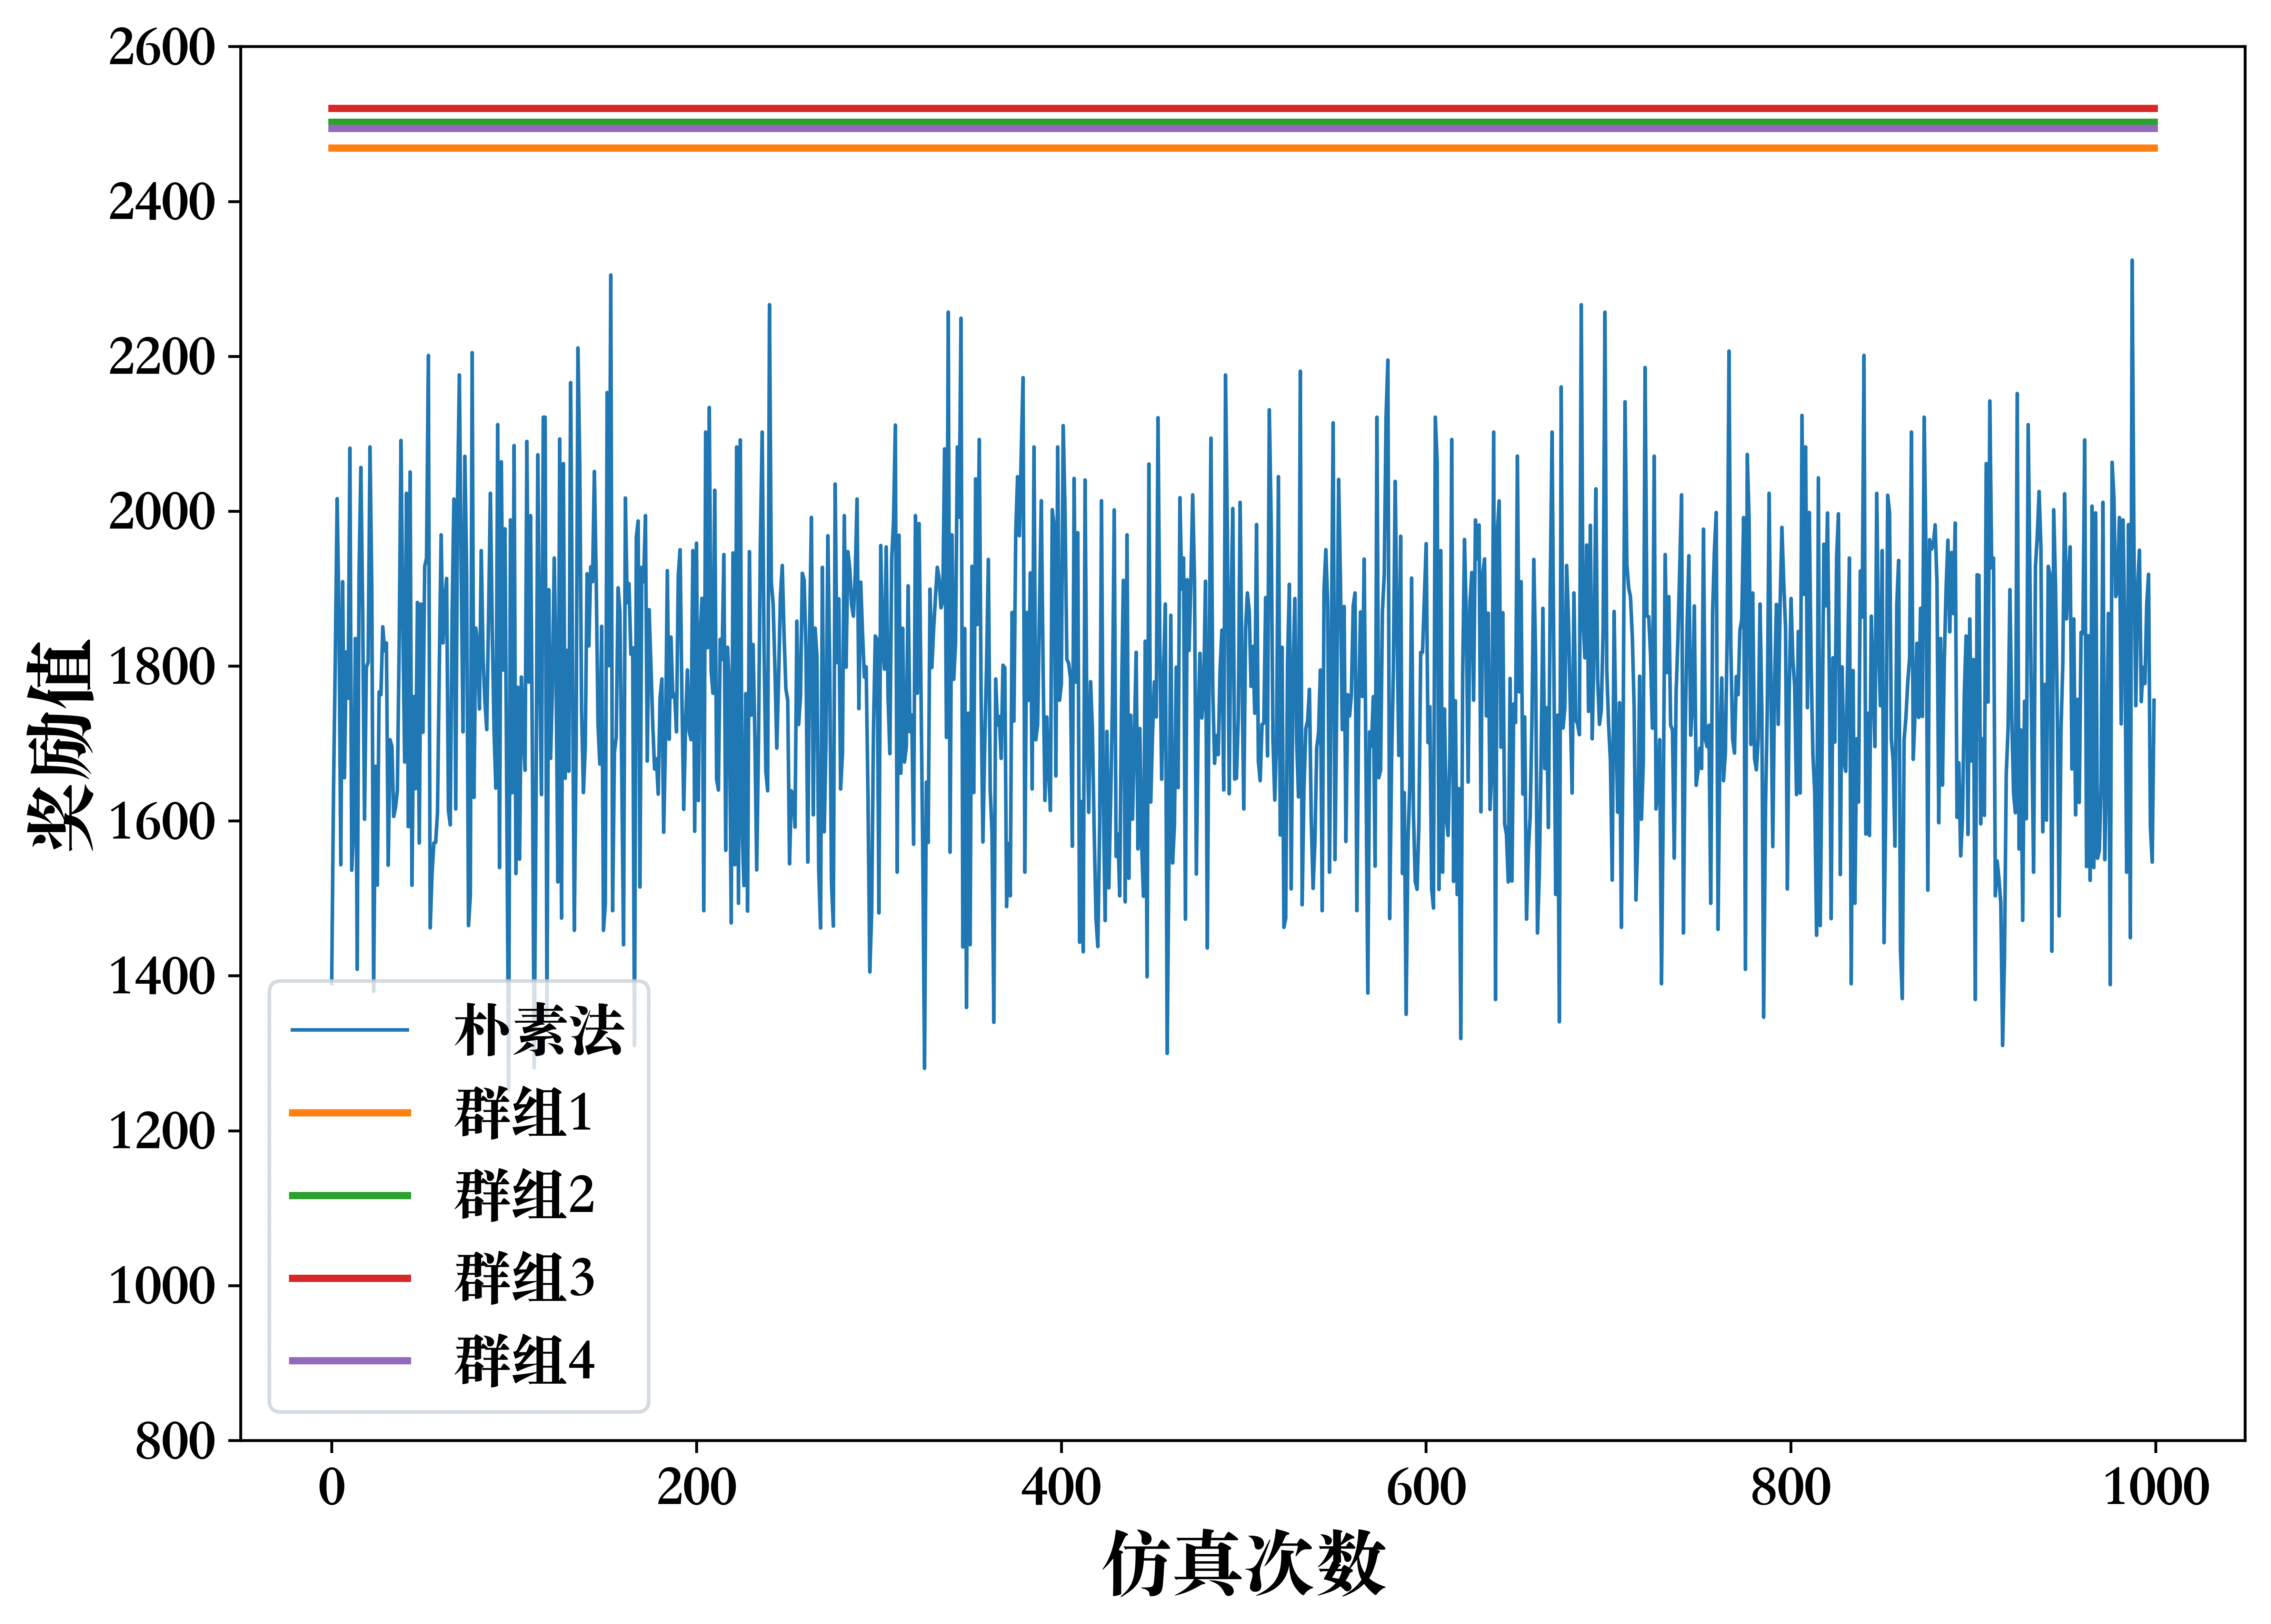
\includegraphics[width=.4\textwidth]{figures/content/agents/agent4.png}}
  \\
  \subfloat[智能体1]{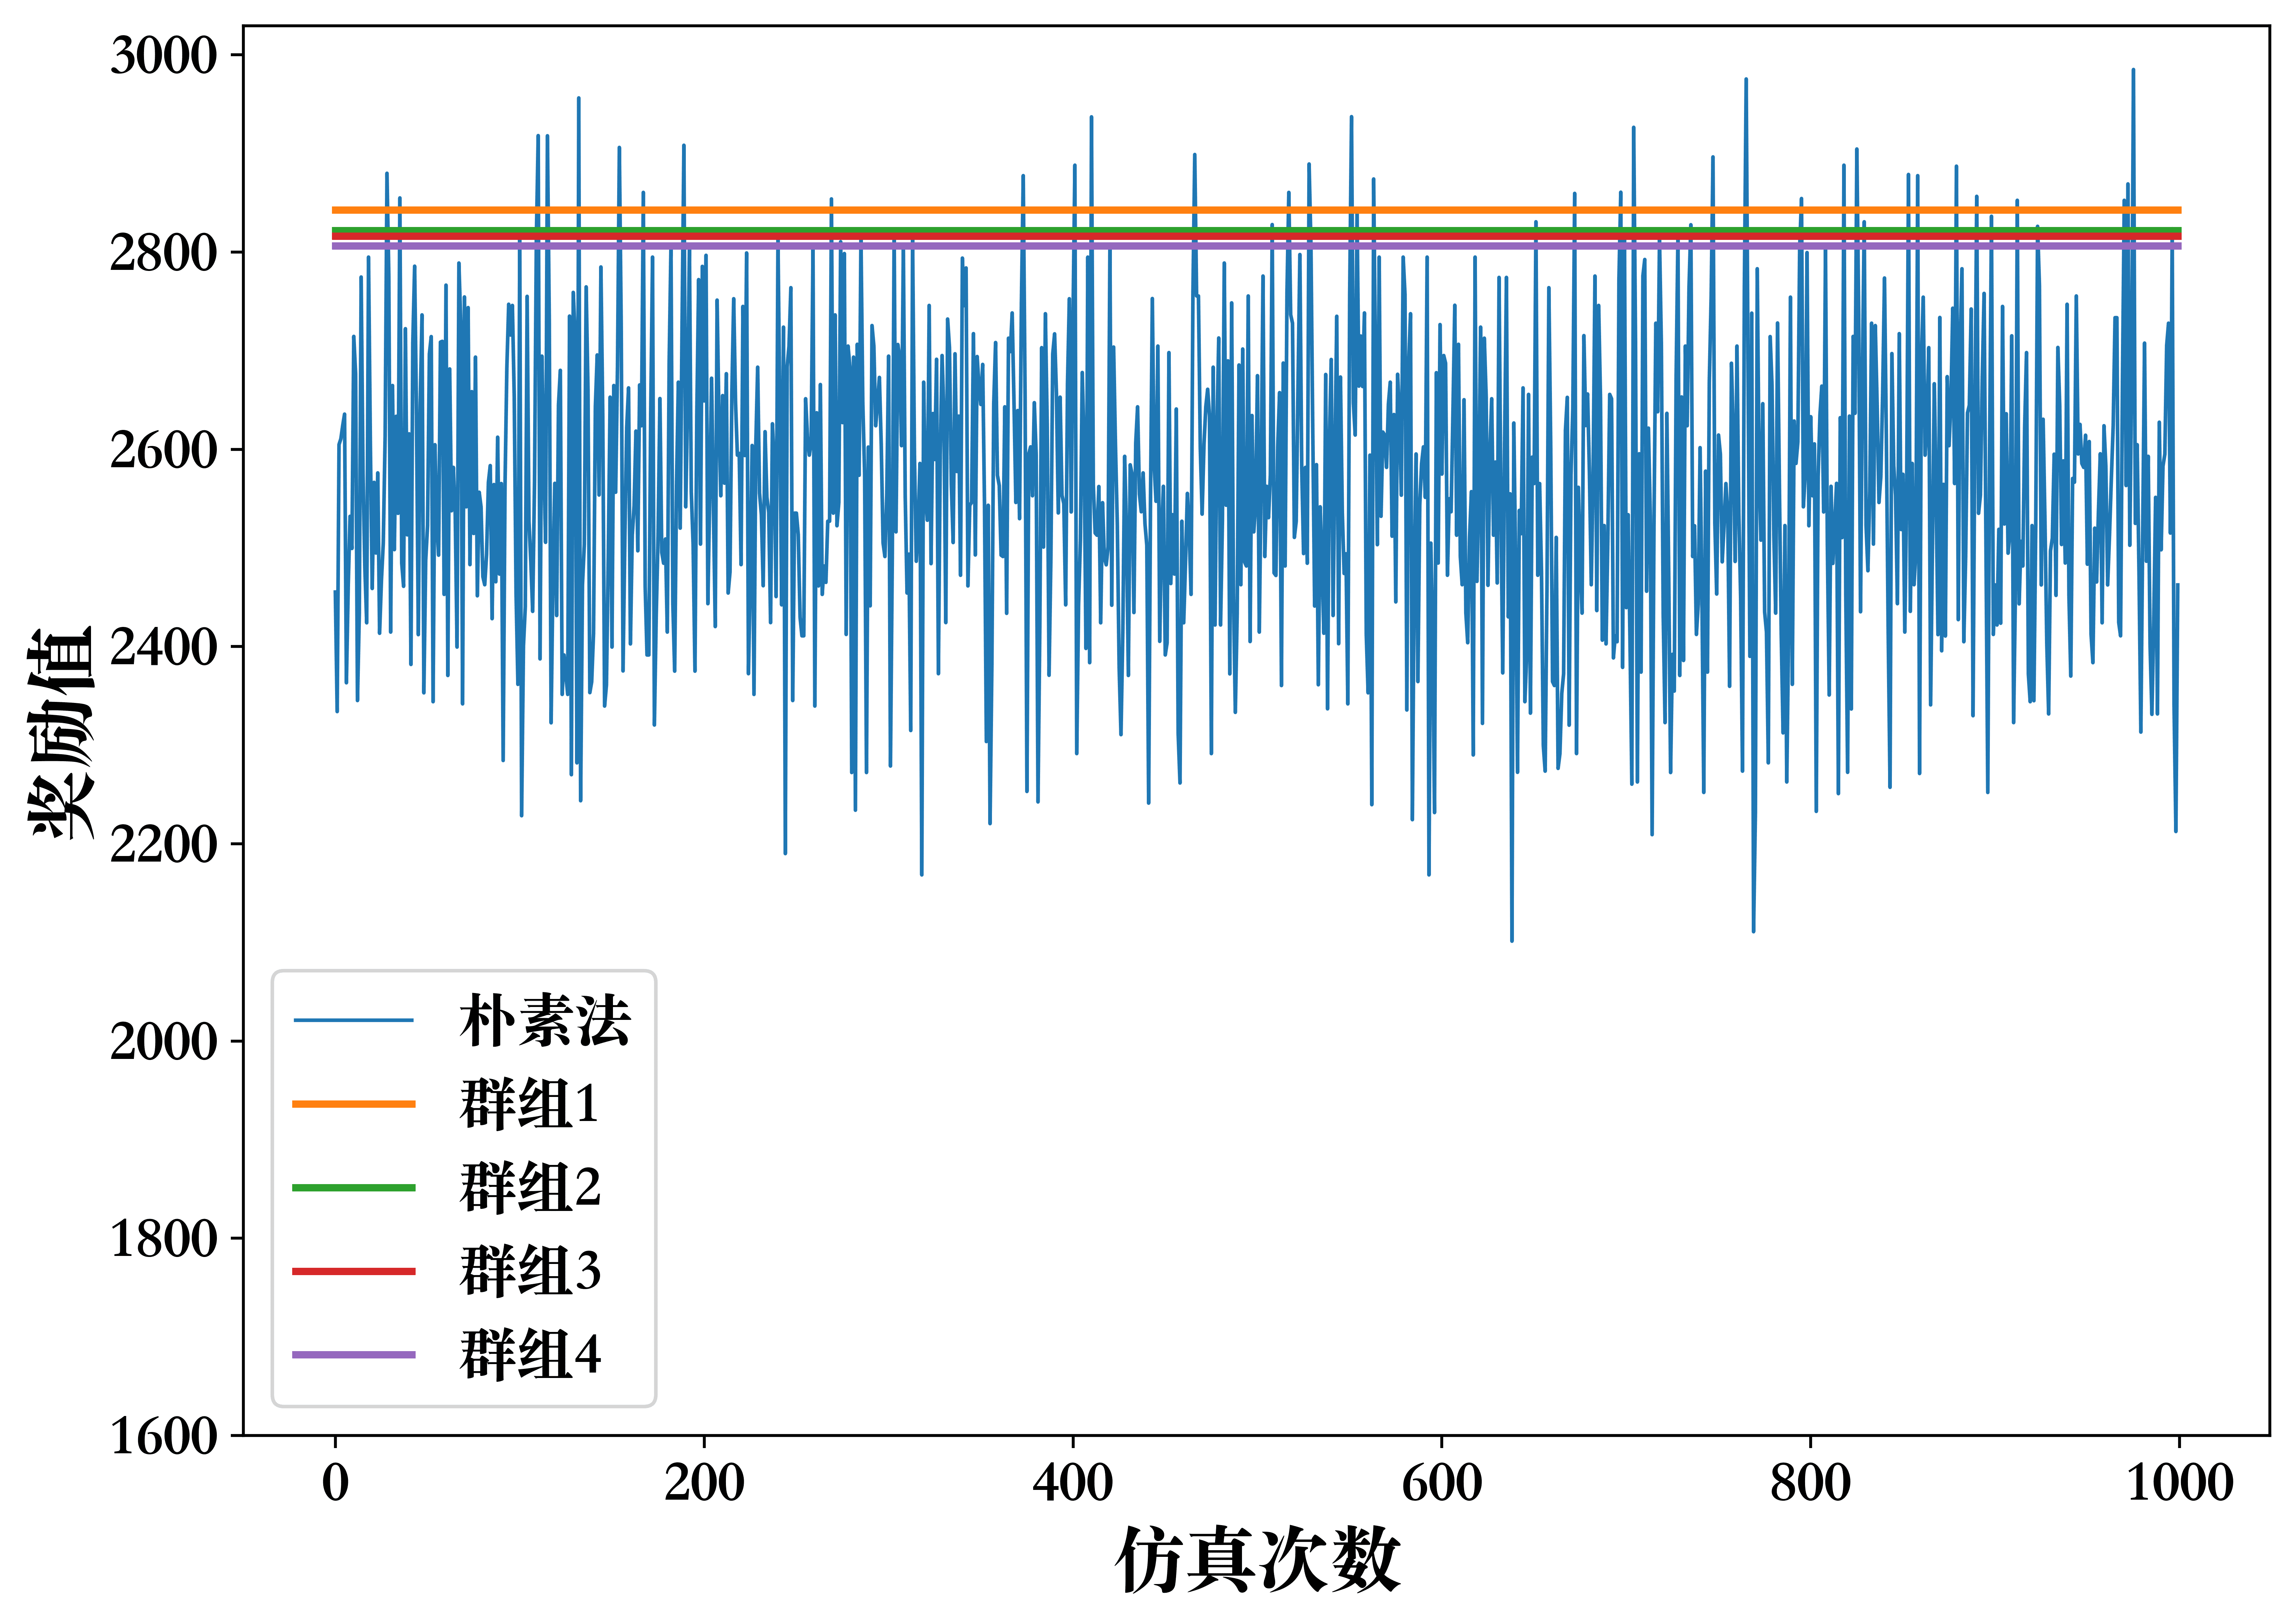
\includegraphics[width=.4\textwidth]{figures/content/agents/agent5.png}}
  \quad\quad
  \subfloat[智能体2]{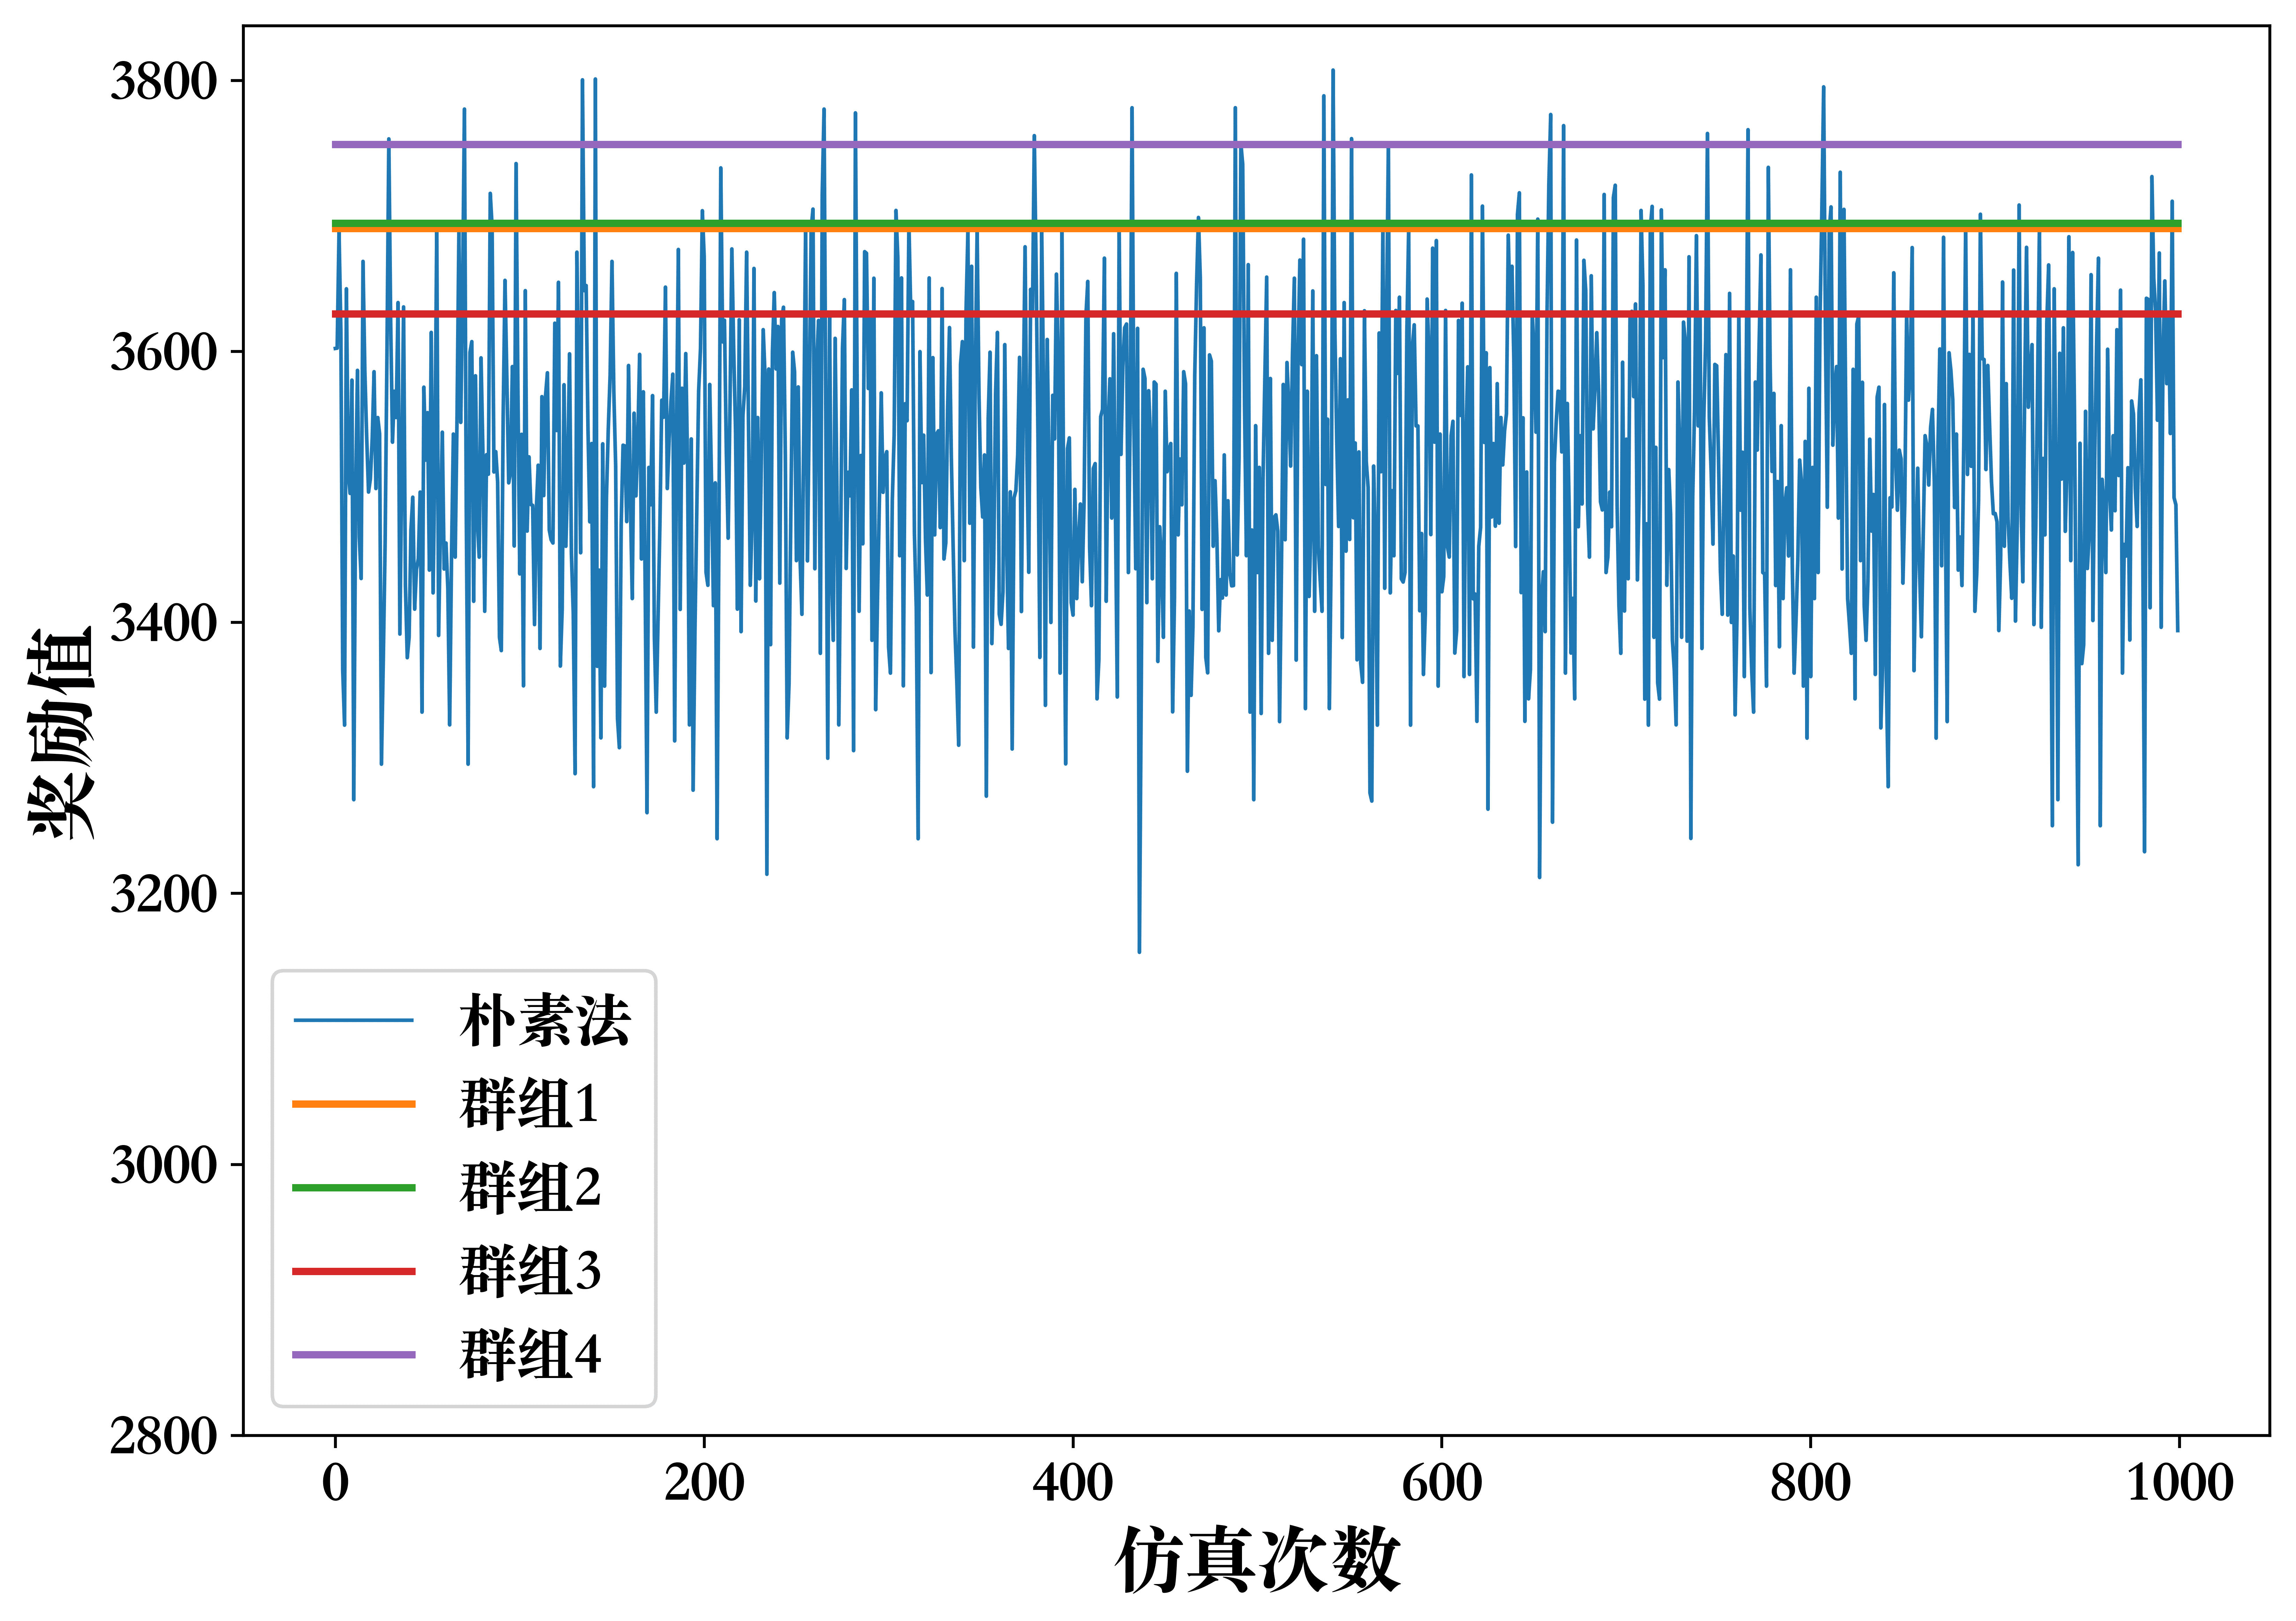
\includegraphics[width=.4\textwidth]{figures/content/agents/agent6.png}}
  \\
  \subfloat[智能体1]{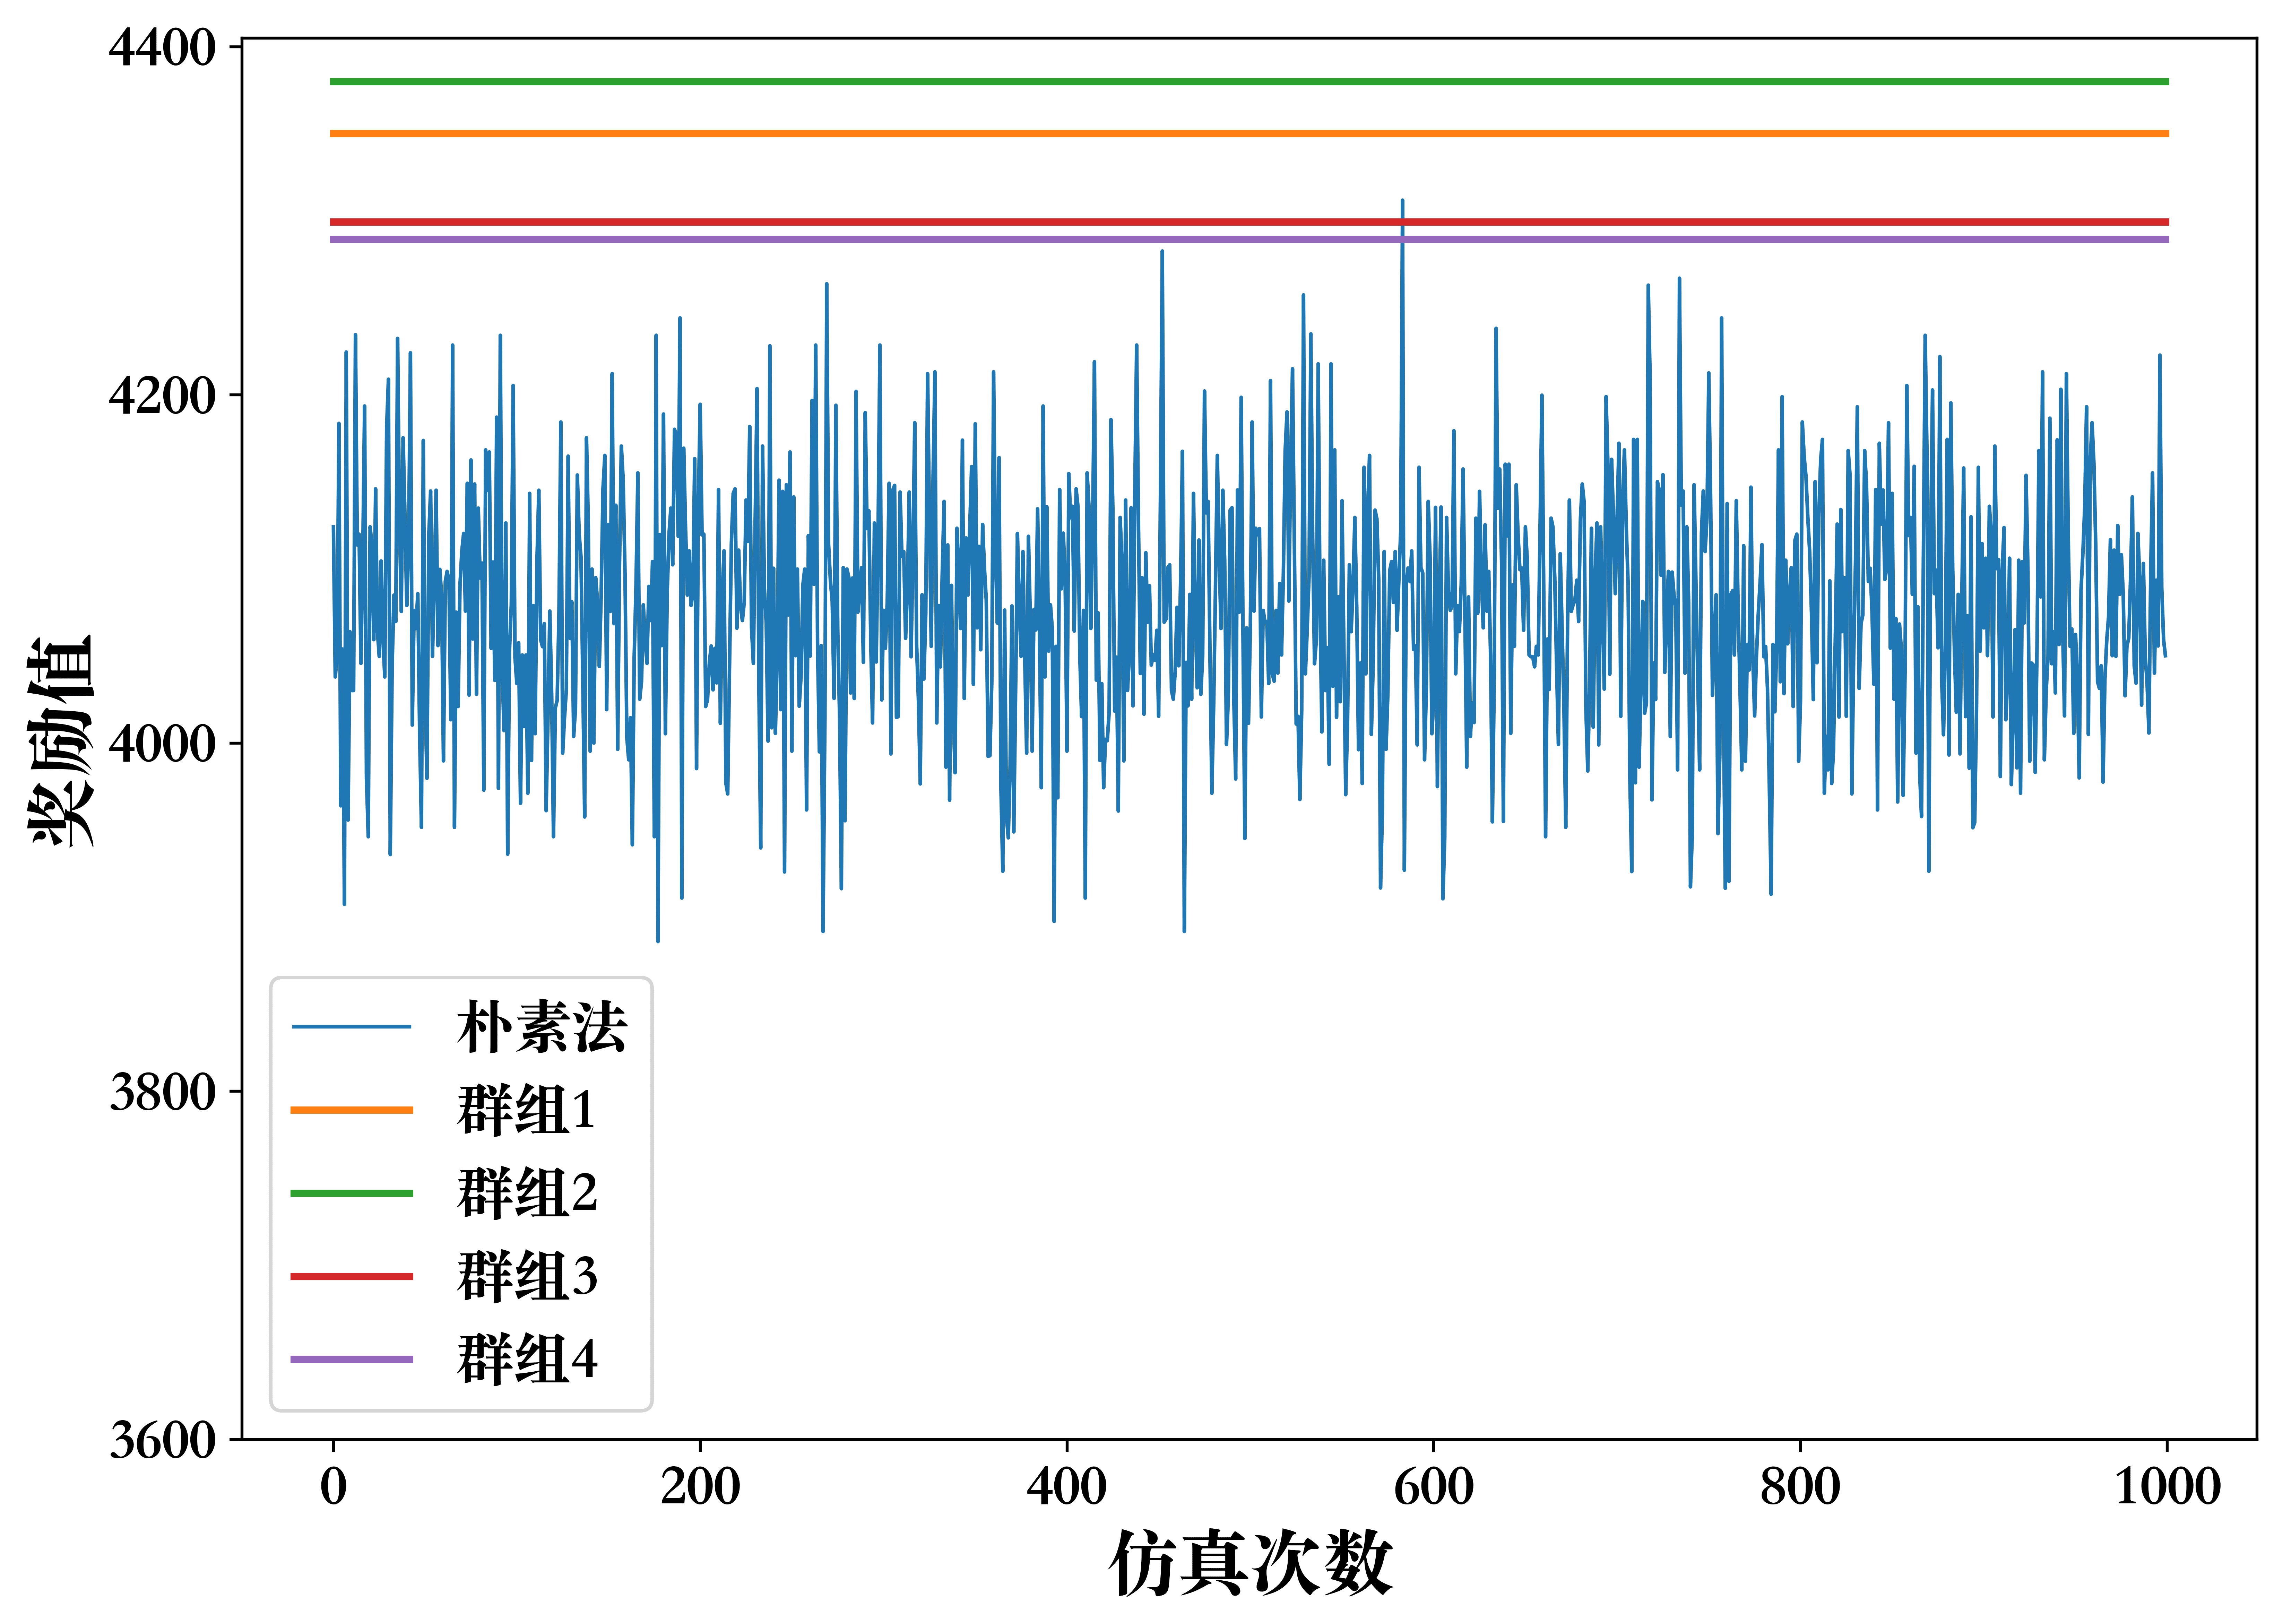
\includegraphics[width=.4\textwidth]{figures/content/agents/agent7.png}}
  \quad\quad
  \subfloat[智能体2]{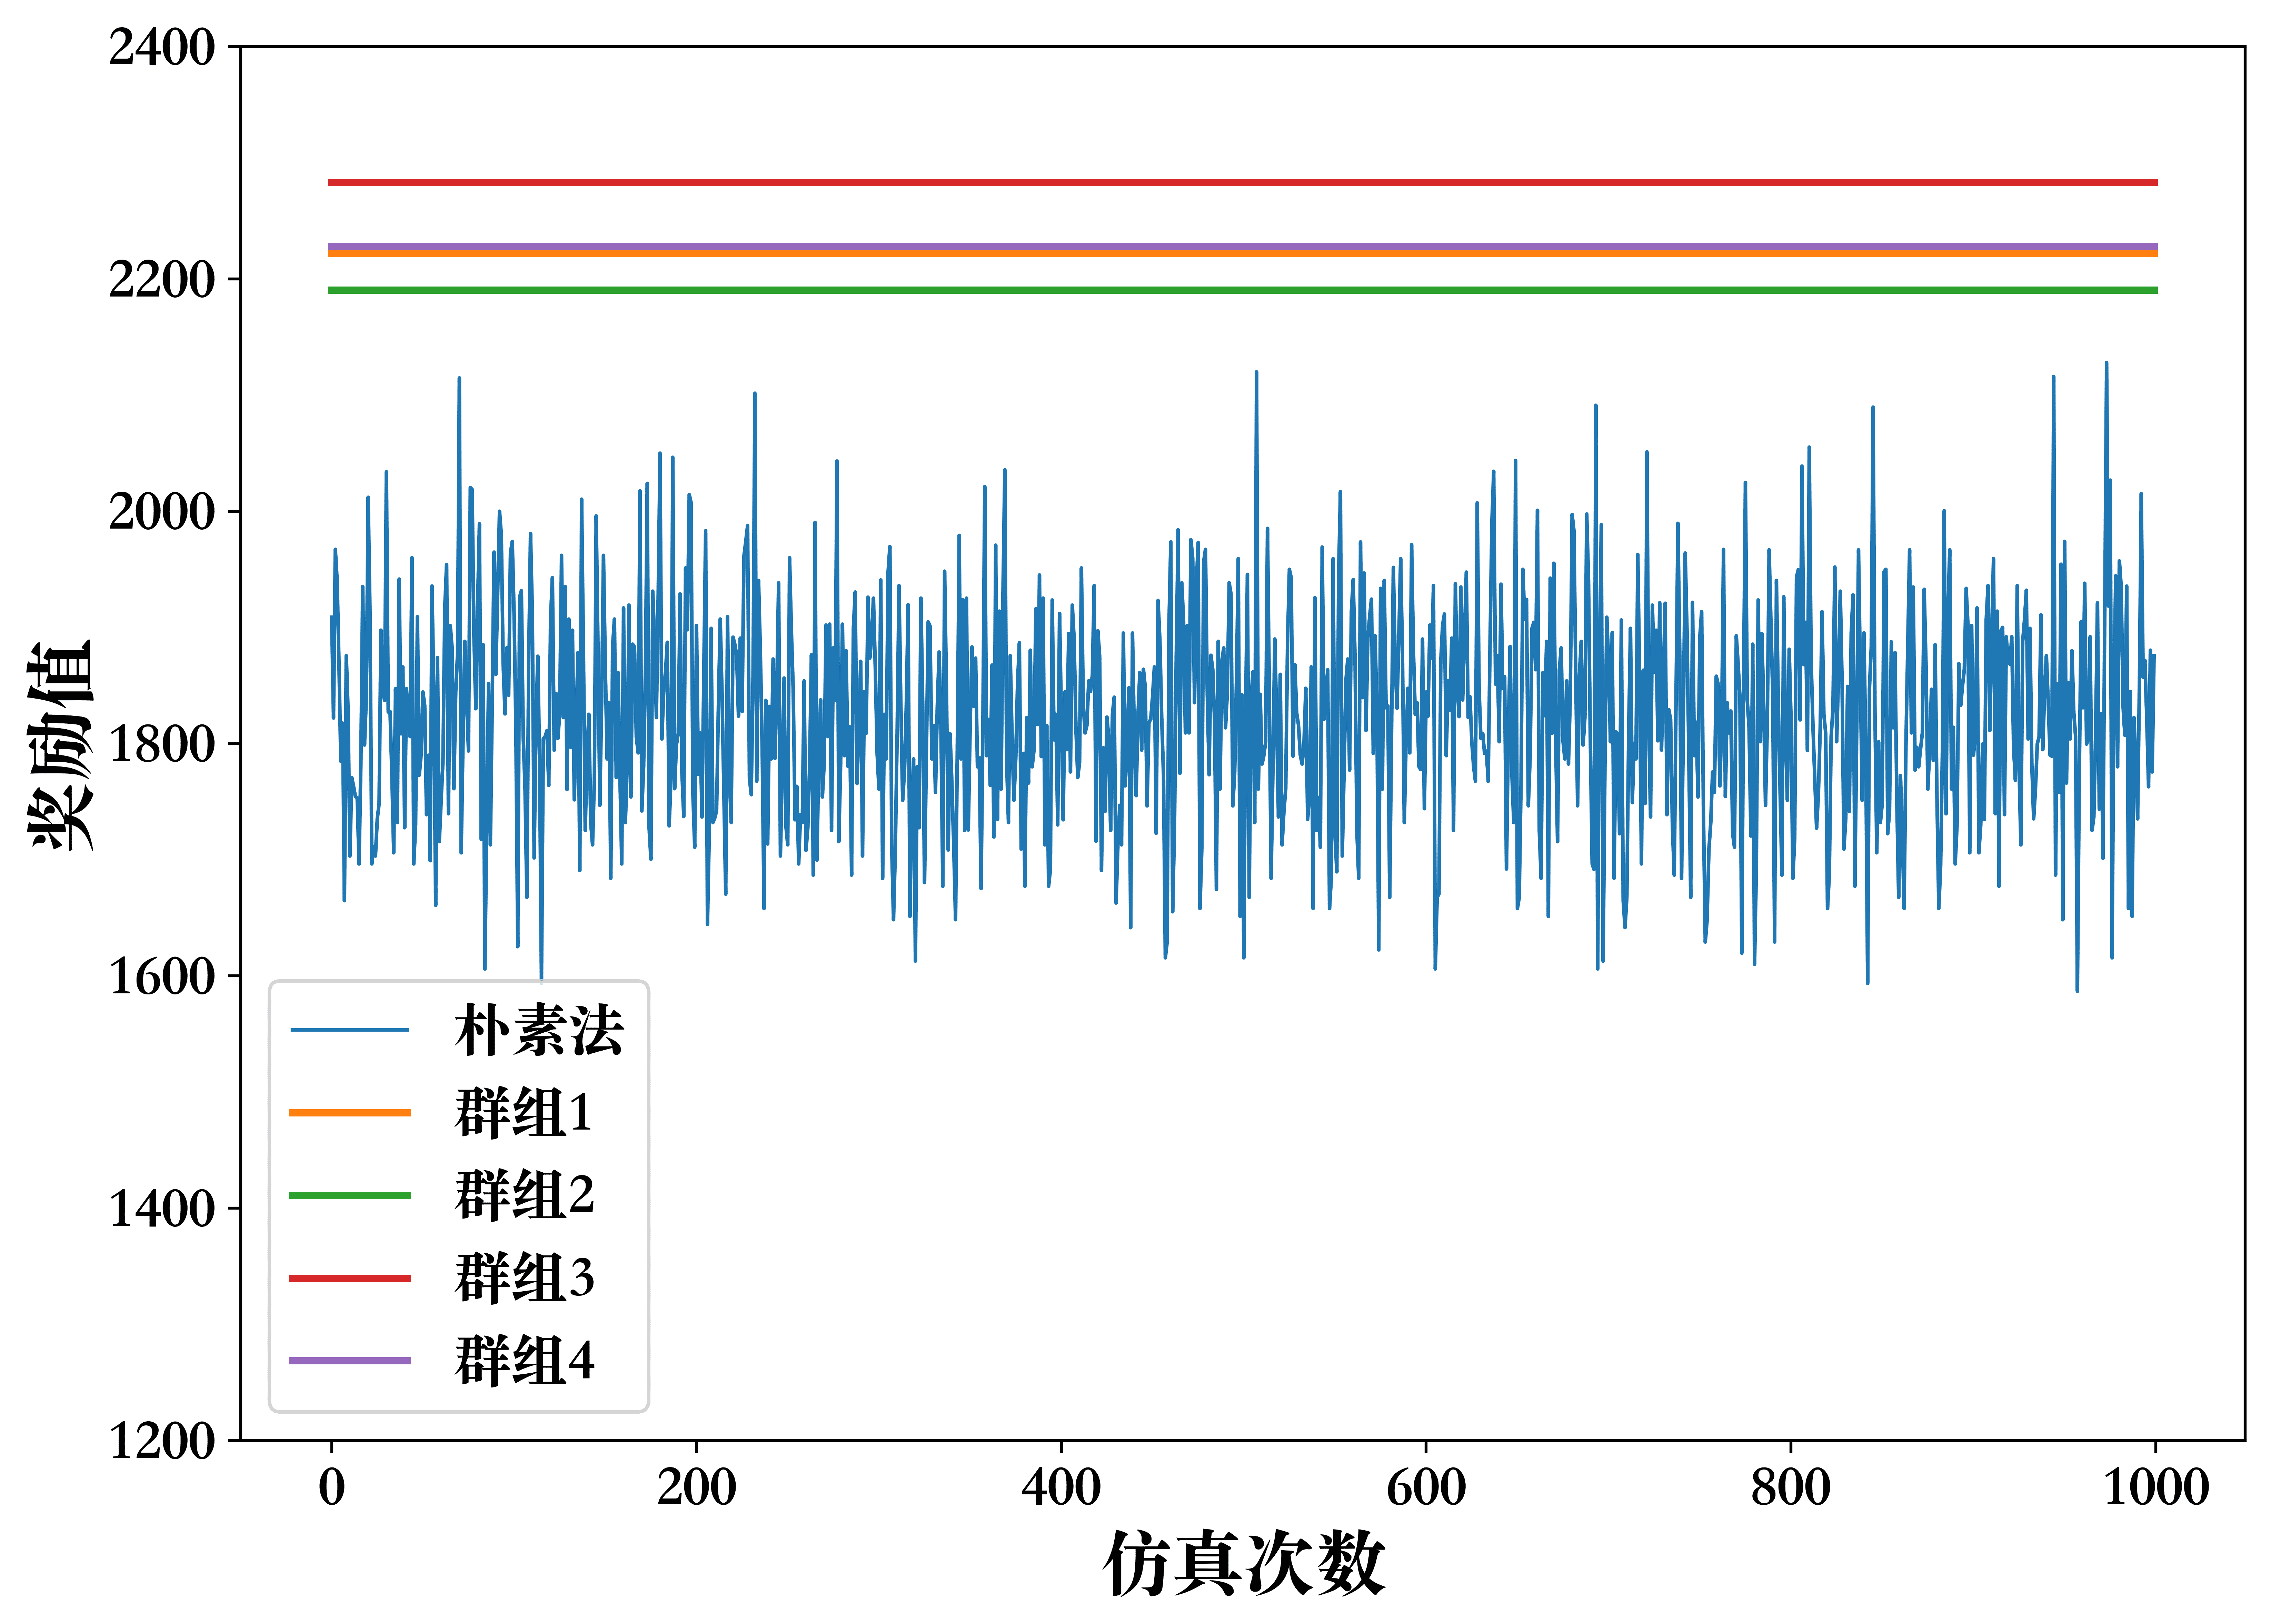
\includegraphics[width=.4\textwidth]{figures/content/agents/agent8.png}}
  \caption{训练过程中代表智能体的动作选择变化}
  \label{agents}
\end{figure}

\begin{table}[htbp]
\centering
\caption{不同代表点数量下所提出方法的性能变化}
\label{cluster_size}
\renewcommand{\arraystretch}{1.2} % 使表格行间距加大1.2倍
\setlength{\tabcolsep}{6mm} % 设置列间距为6mm
\small % 调整字体大小为small

\begin{tabular}{lccccc}
\toprule
代表点数量     & 1  & 4  & 10 & 20  & 40                \\ \midrule
训练时间 (小时)  & 5        & 22        & 68         & 140        & \textbackslash{}       \\
平均奖励值 & 2,684      & 3,203      & 3,351       & 3,394        & \textbackslash{}   \\
超过95(共50次)的次数     & 16        & 41         & 45          & 46          & \textbackslash{}\\ \bottomrule
\end{tabular}
\end{table}


为了显示所提出方法的性能并不因训练个体的不同而发生显著变化,我们使用不同的训练个体集合进行另一组实验,使用四个代表对DQN进行训练,其余的实验设置保持不变。表\ref{cluster_agents}总结了这样四个实验的结果。由于不同的训练个体集合不会改变计算时间(对于四个代表,计算时间为22小时),因此不再报告这个度量。从结果中可以看出,所提出方法的性能是稳定的,不会因为用于训练的代表个体不同而表现出显著的变化。类似于图\ref{appendixa1},图\ref{appendixb1}显示了当使用不同的训练个体集合时,四个选定测试个体结果的比较,表明所提出的方法对代表个体的选择具有鲁棒性。这些结果表明,所提出的方法是有效的,不会受到训练代表个体集合的影响。从这些敏感性分析中可以得出结论,所提出的方法在实际应用中具有很强的可操作性和鲁棒性。通过将模型应用于新的时间依赖 OD 数据集并比较与传统模型和暴力方法的性能,我们证明了该方法在解决 JTMDTC 问题方面的有效性。

\begin{figure}[htbp]
  \subfloat[智能体1]{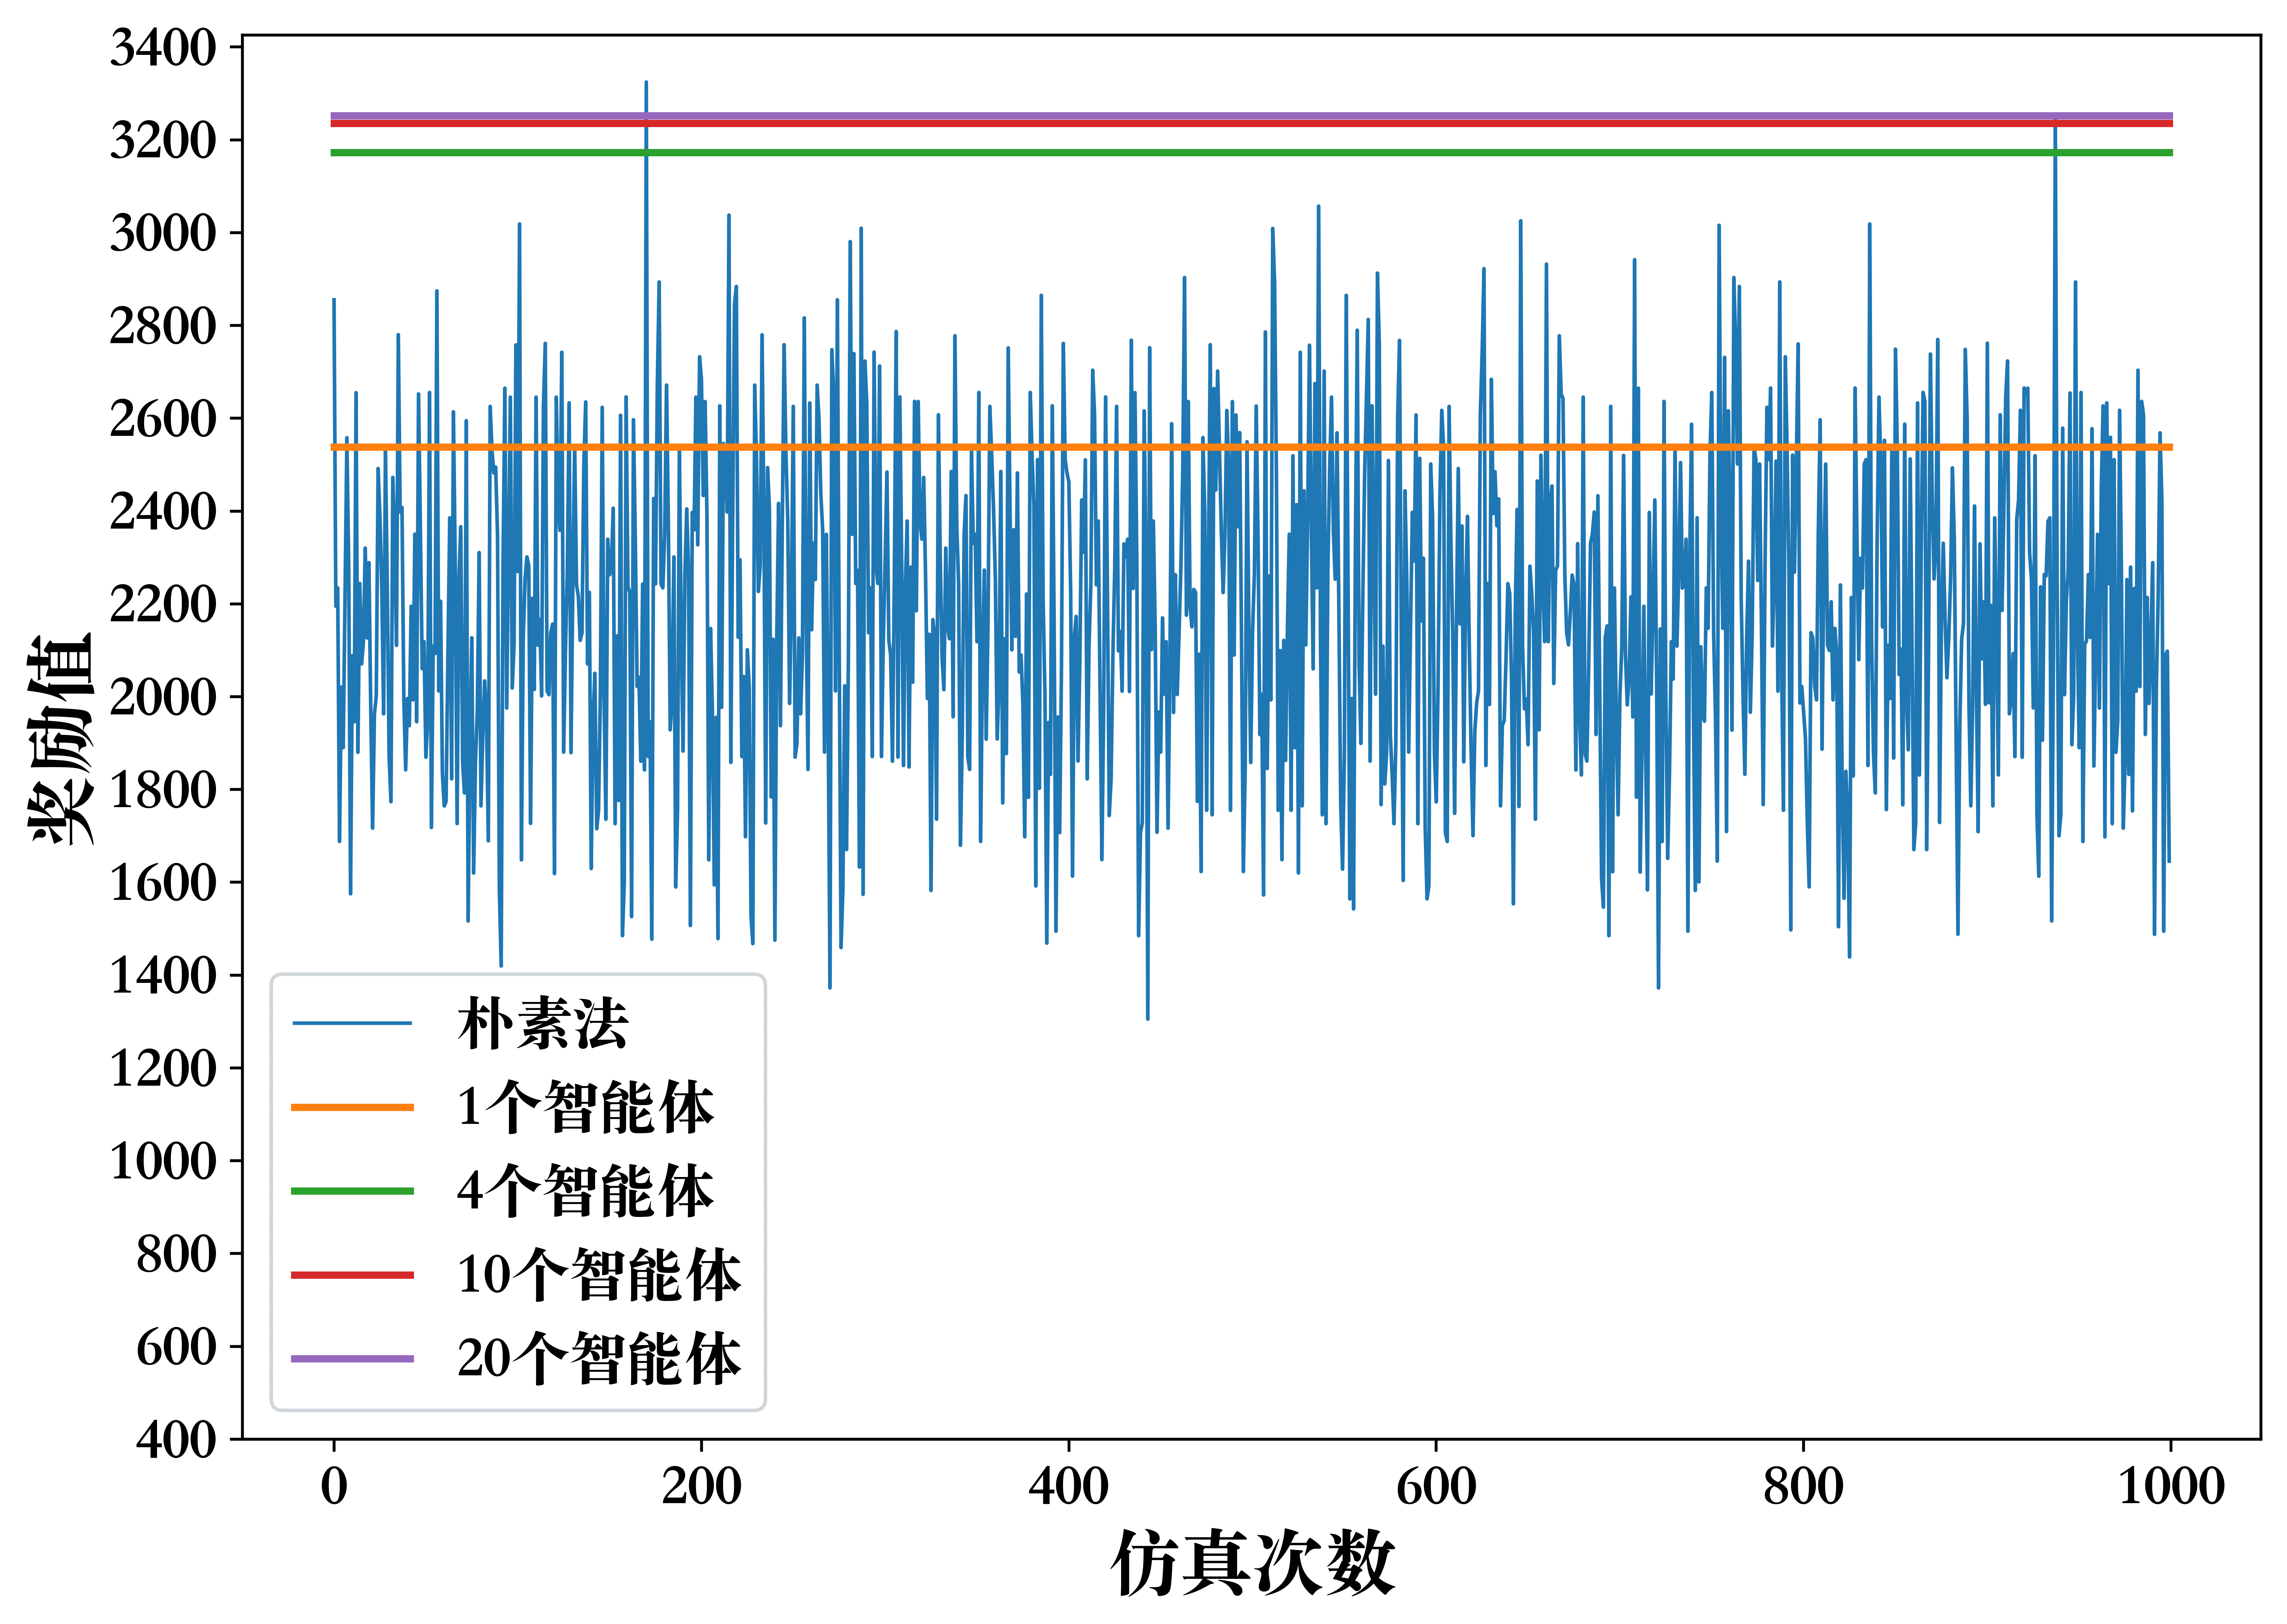
\includegraphics[width=.4\textwidth]{figures/content/size/size1.png}}
  \quad\quad
  \subfloat[智能体2]{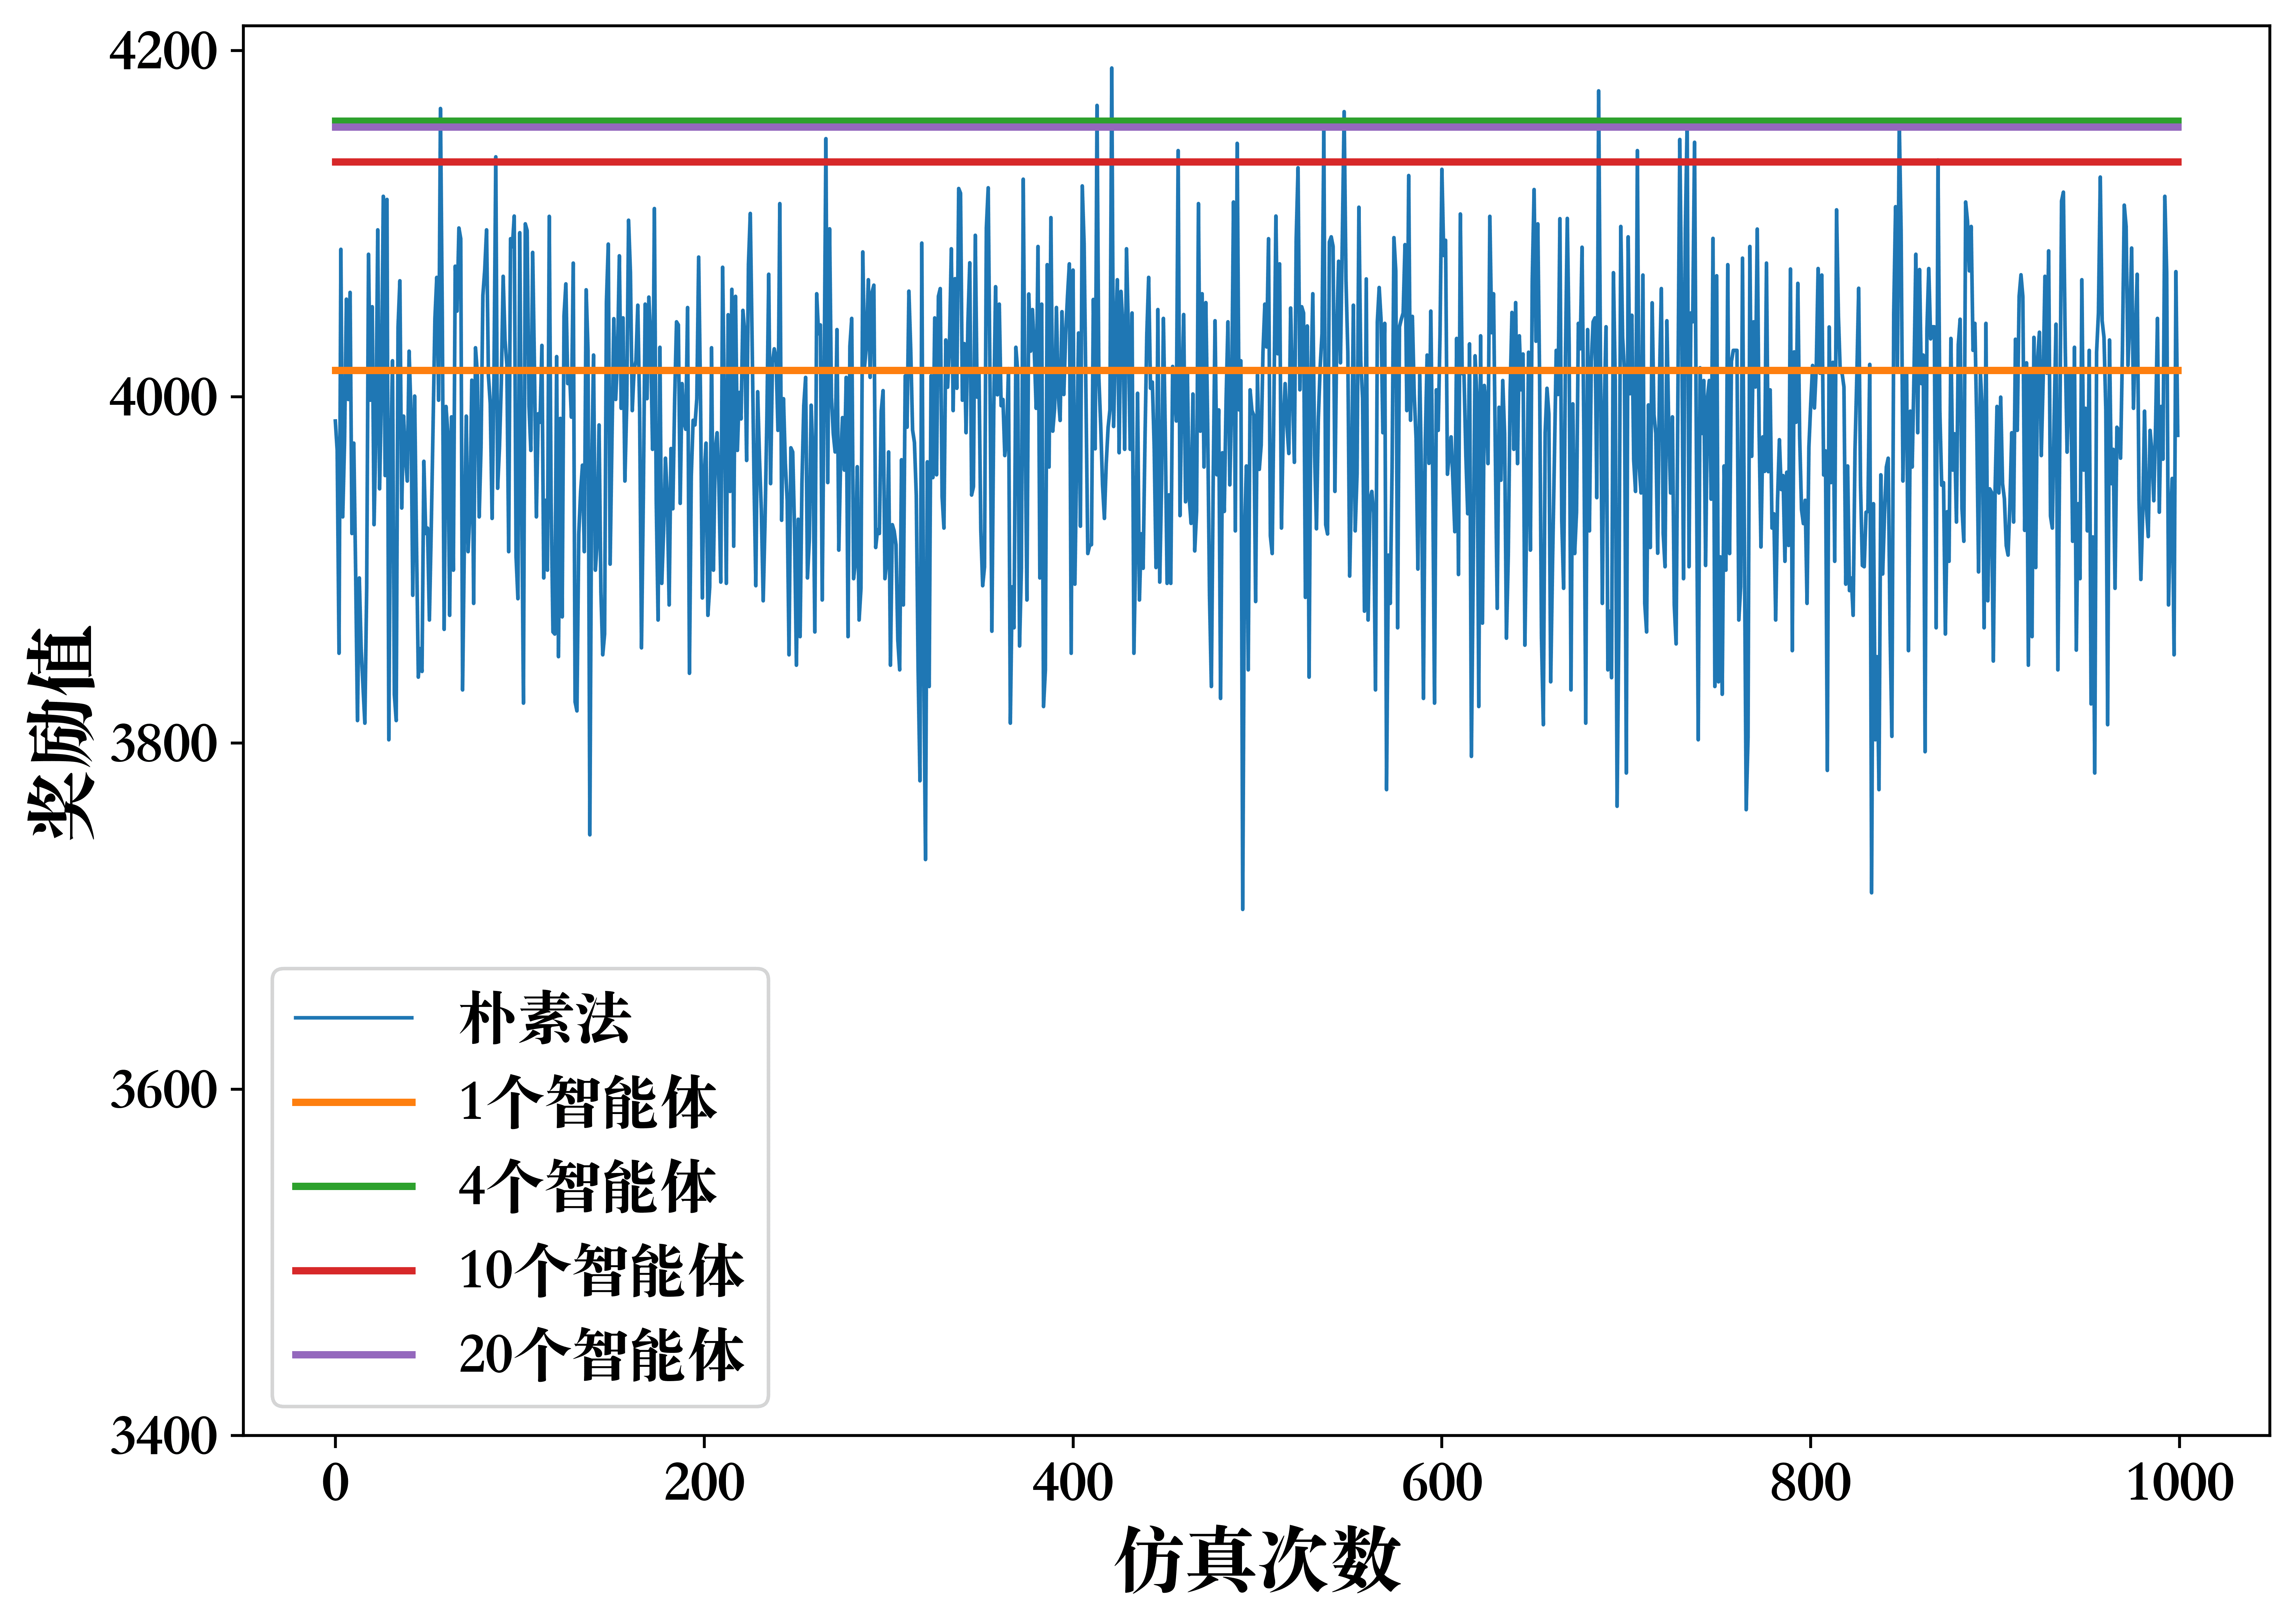
\includegraphics[width=.4\textwidth]{figures/content/size/size2.png}}
  \\
  \subfloat[智能体3]{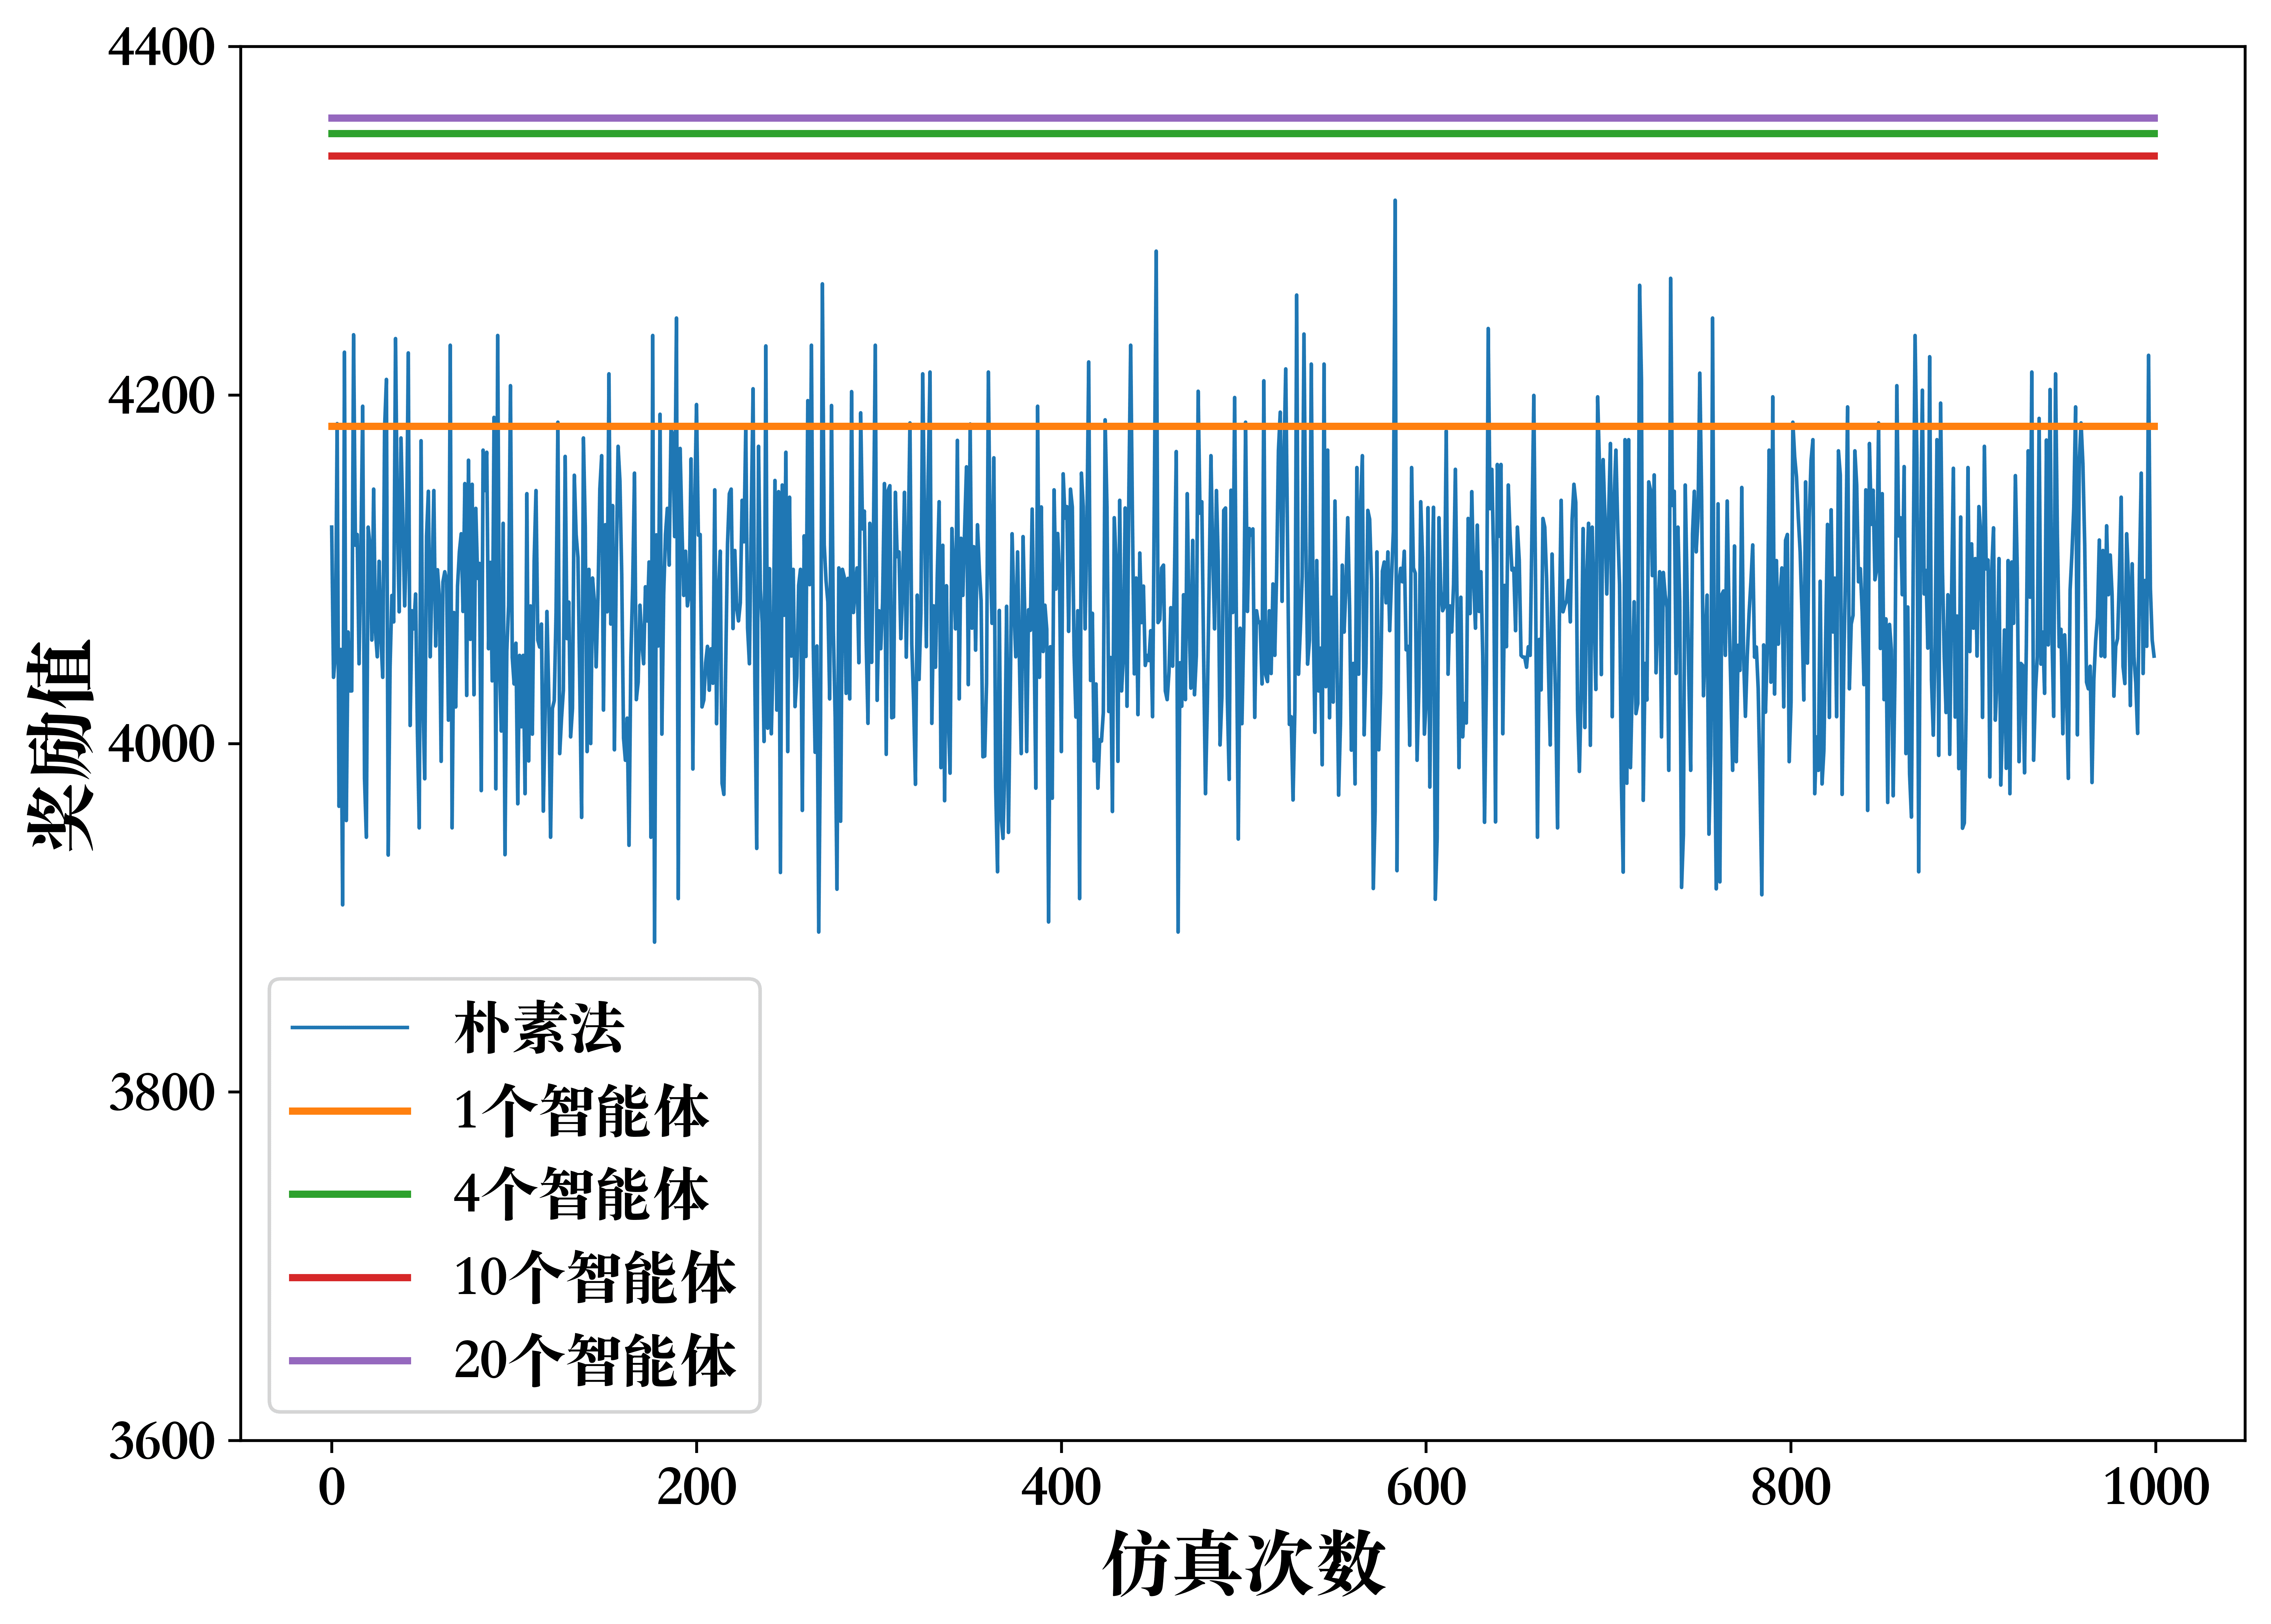
\includegraphics[width=.4\textwidth]{figures/content/size/size3.png}}
  \quad\quad
  \subfloat[智能体4]{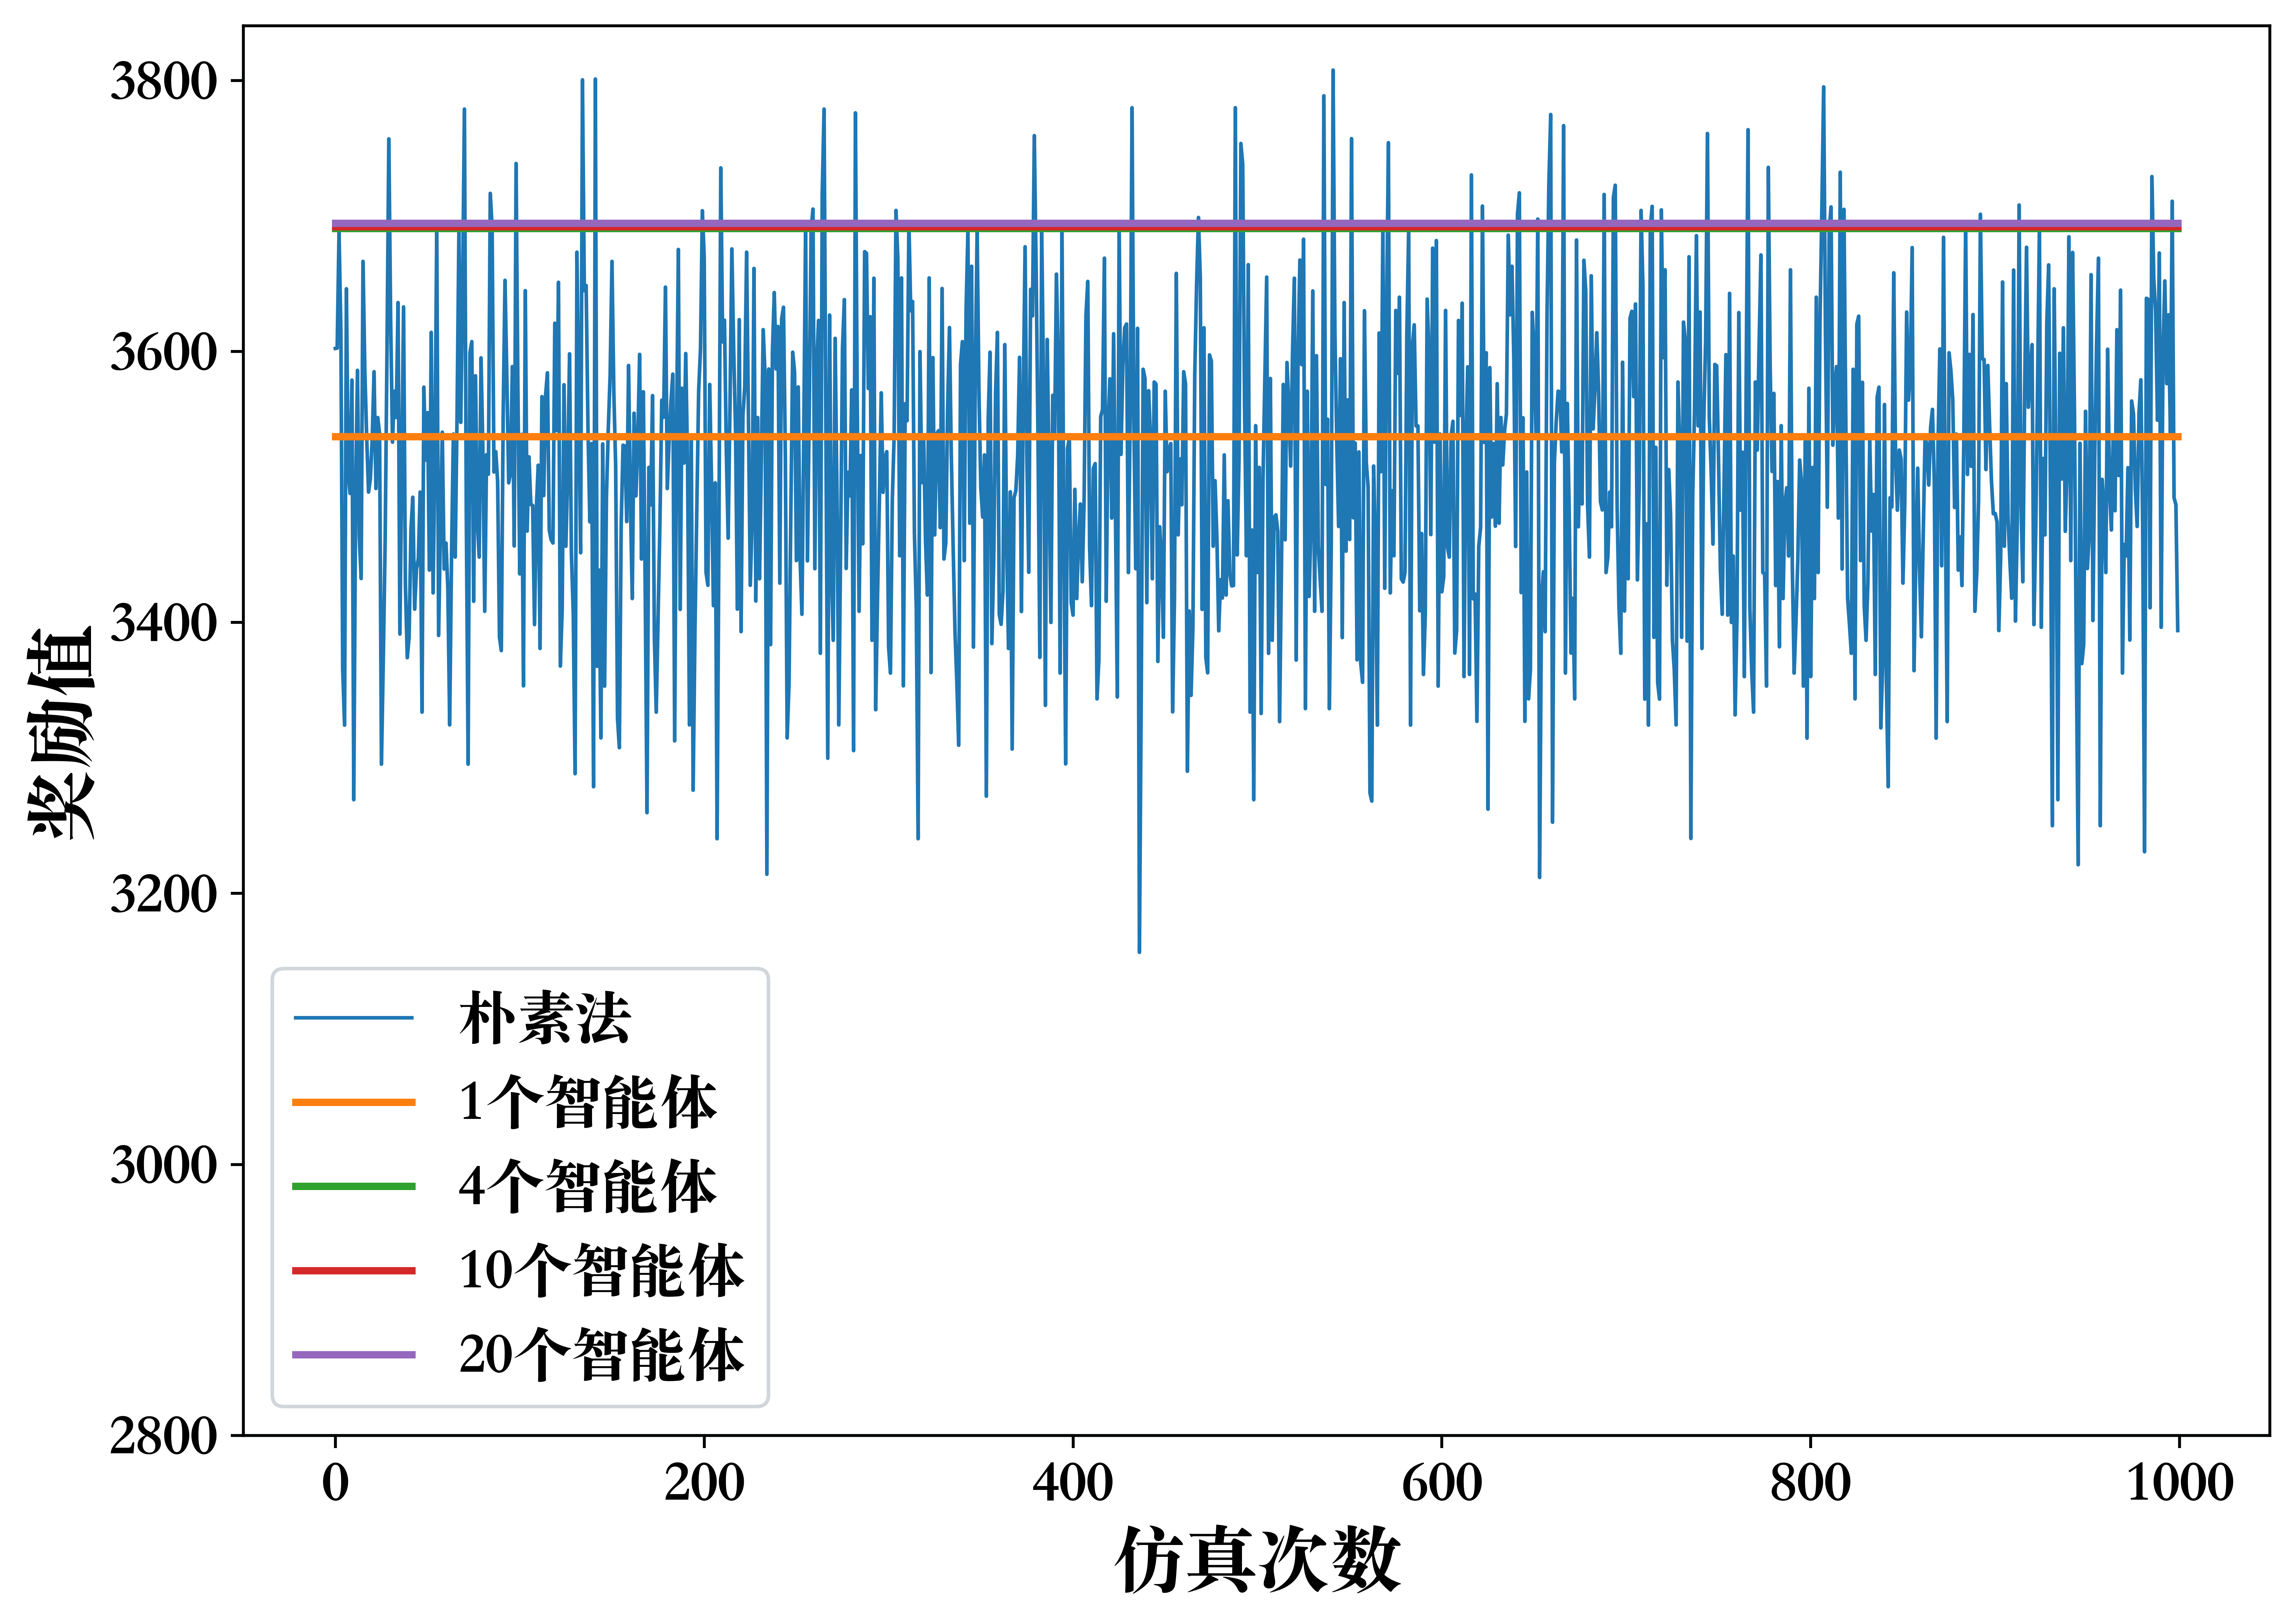
\includegraphics[width=.4\textwidth]{figures/content/size/size4.png}}
  \\
  \subfloat[智能体1]{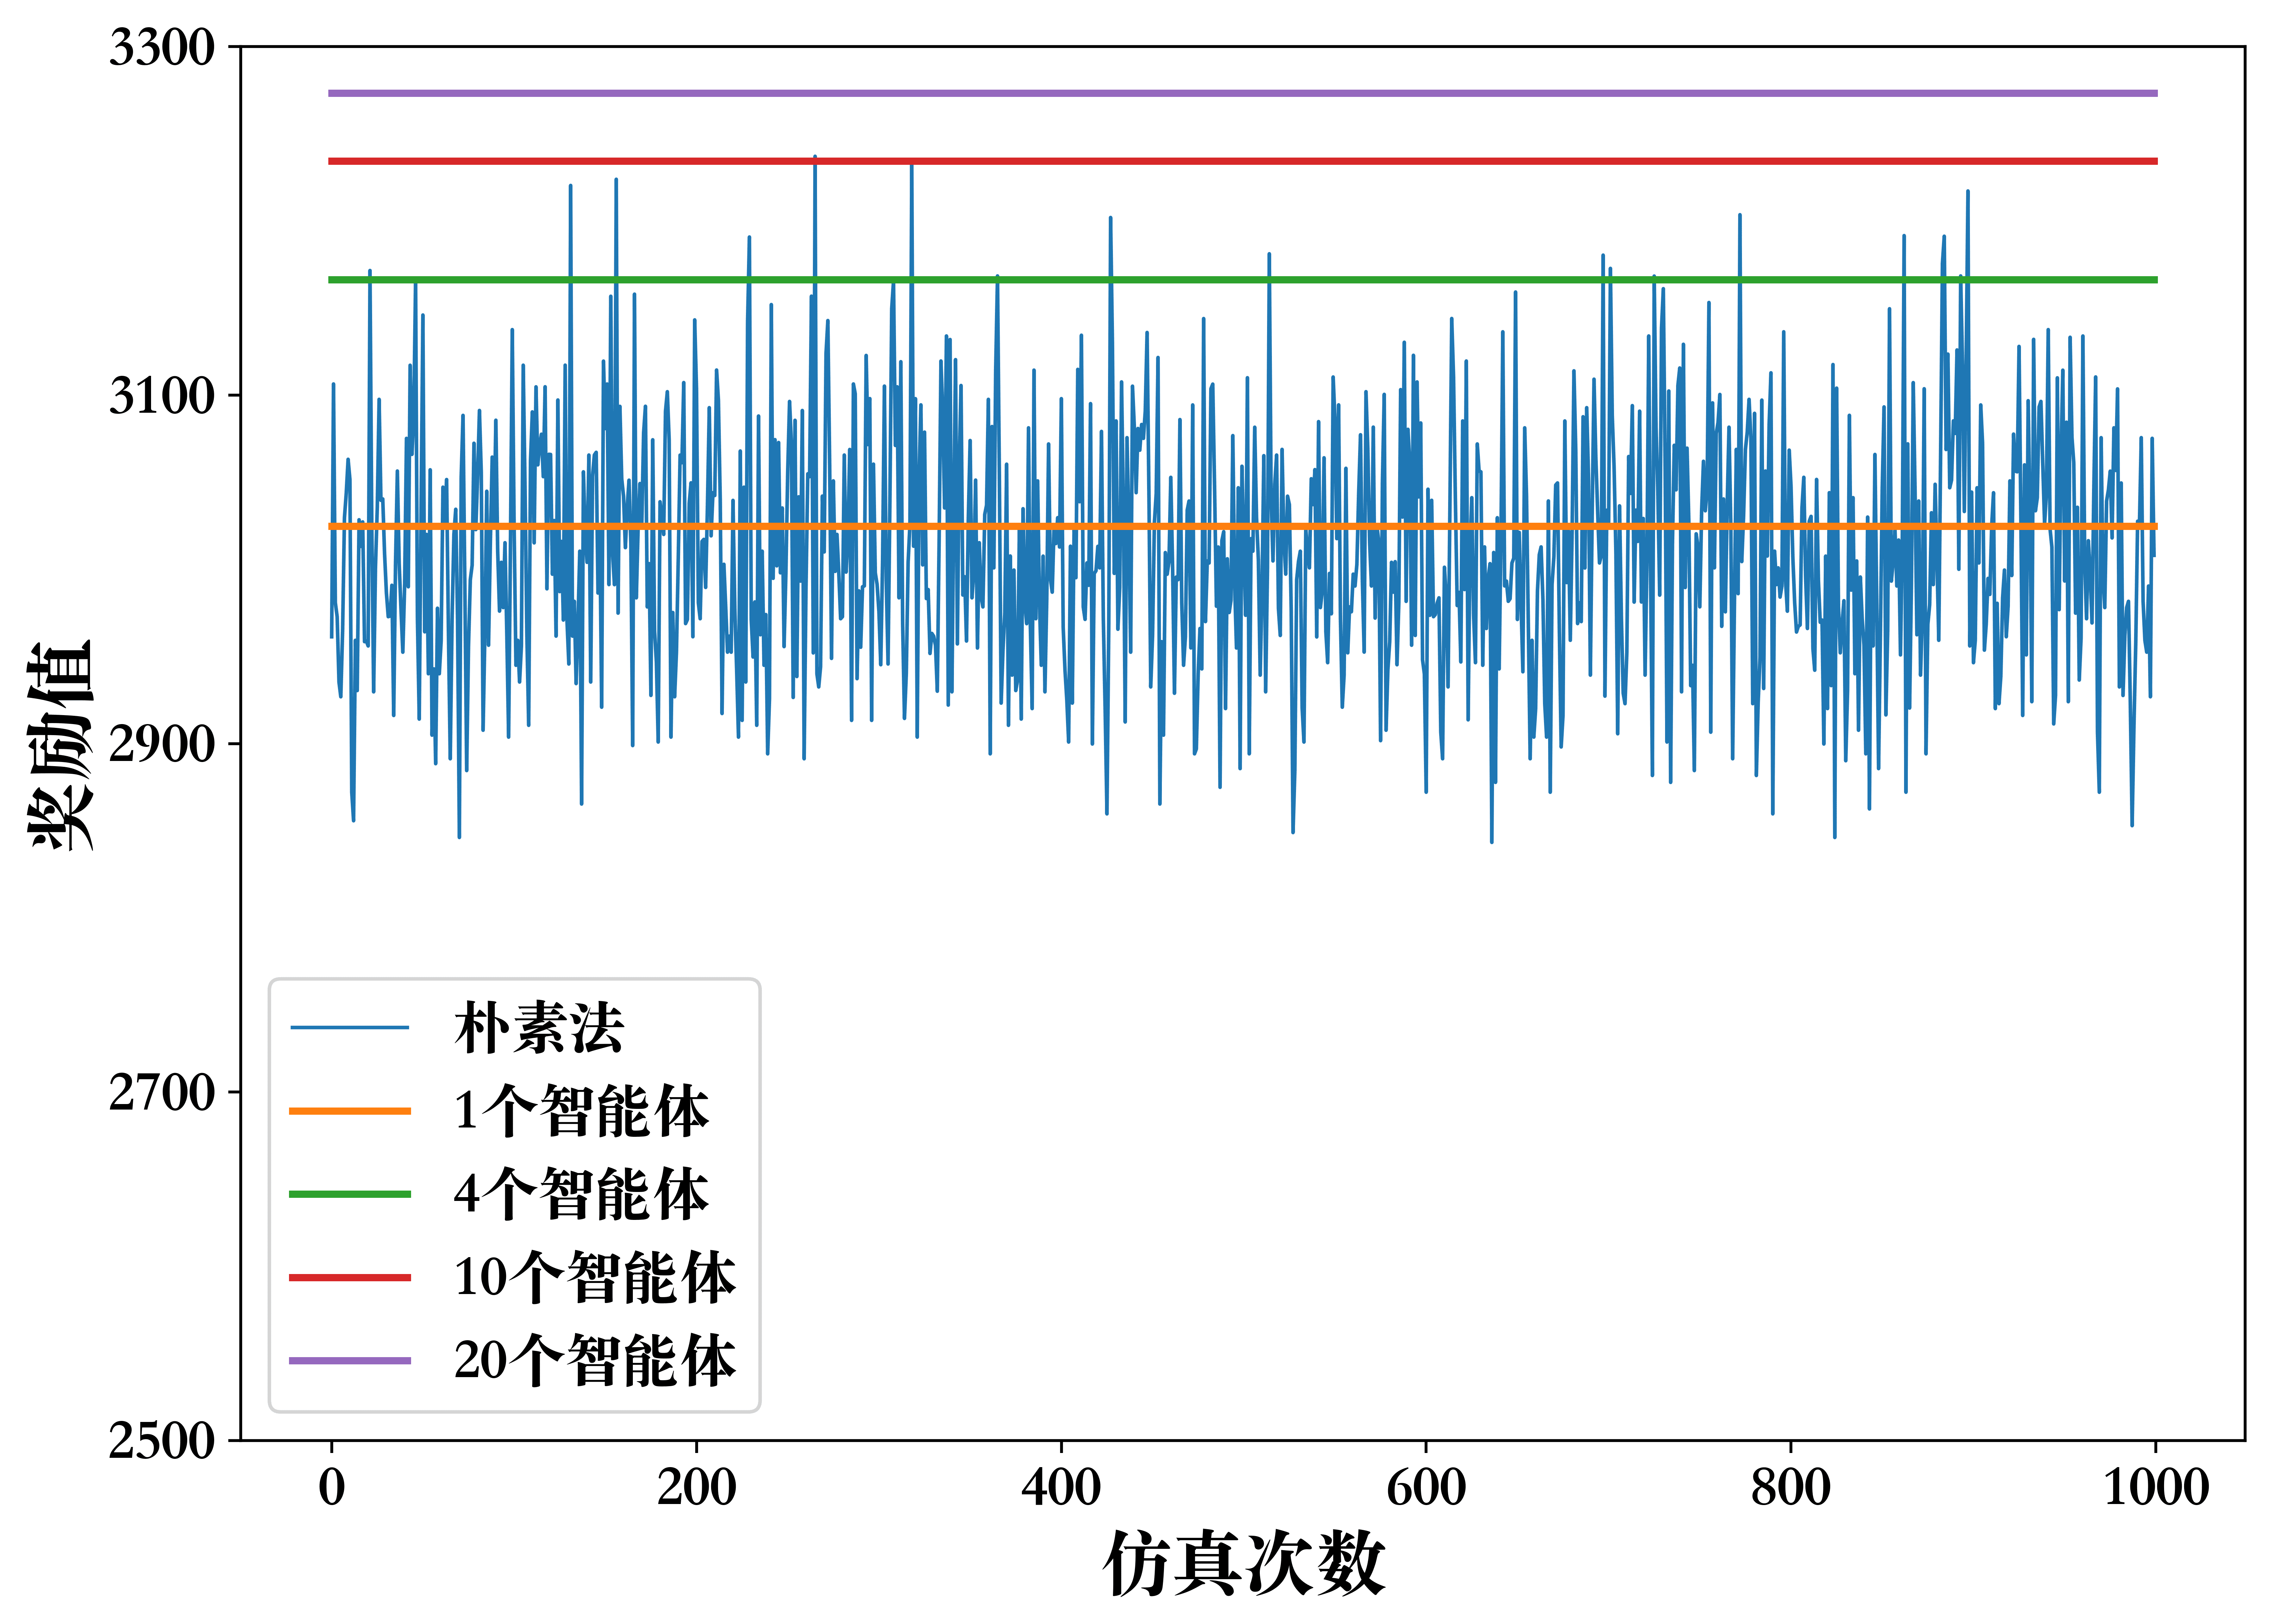
\includegraphics[width=.4\textwidth]{figures/content/size/size5.png}}
  \quad\quad
  \subfloat[智能体2]{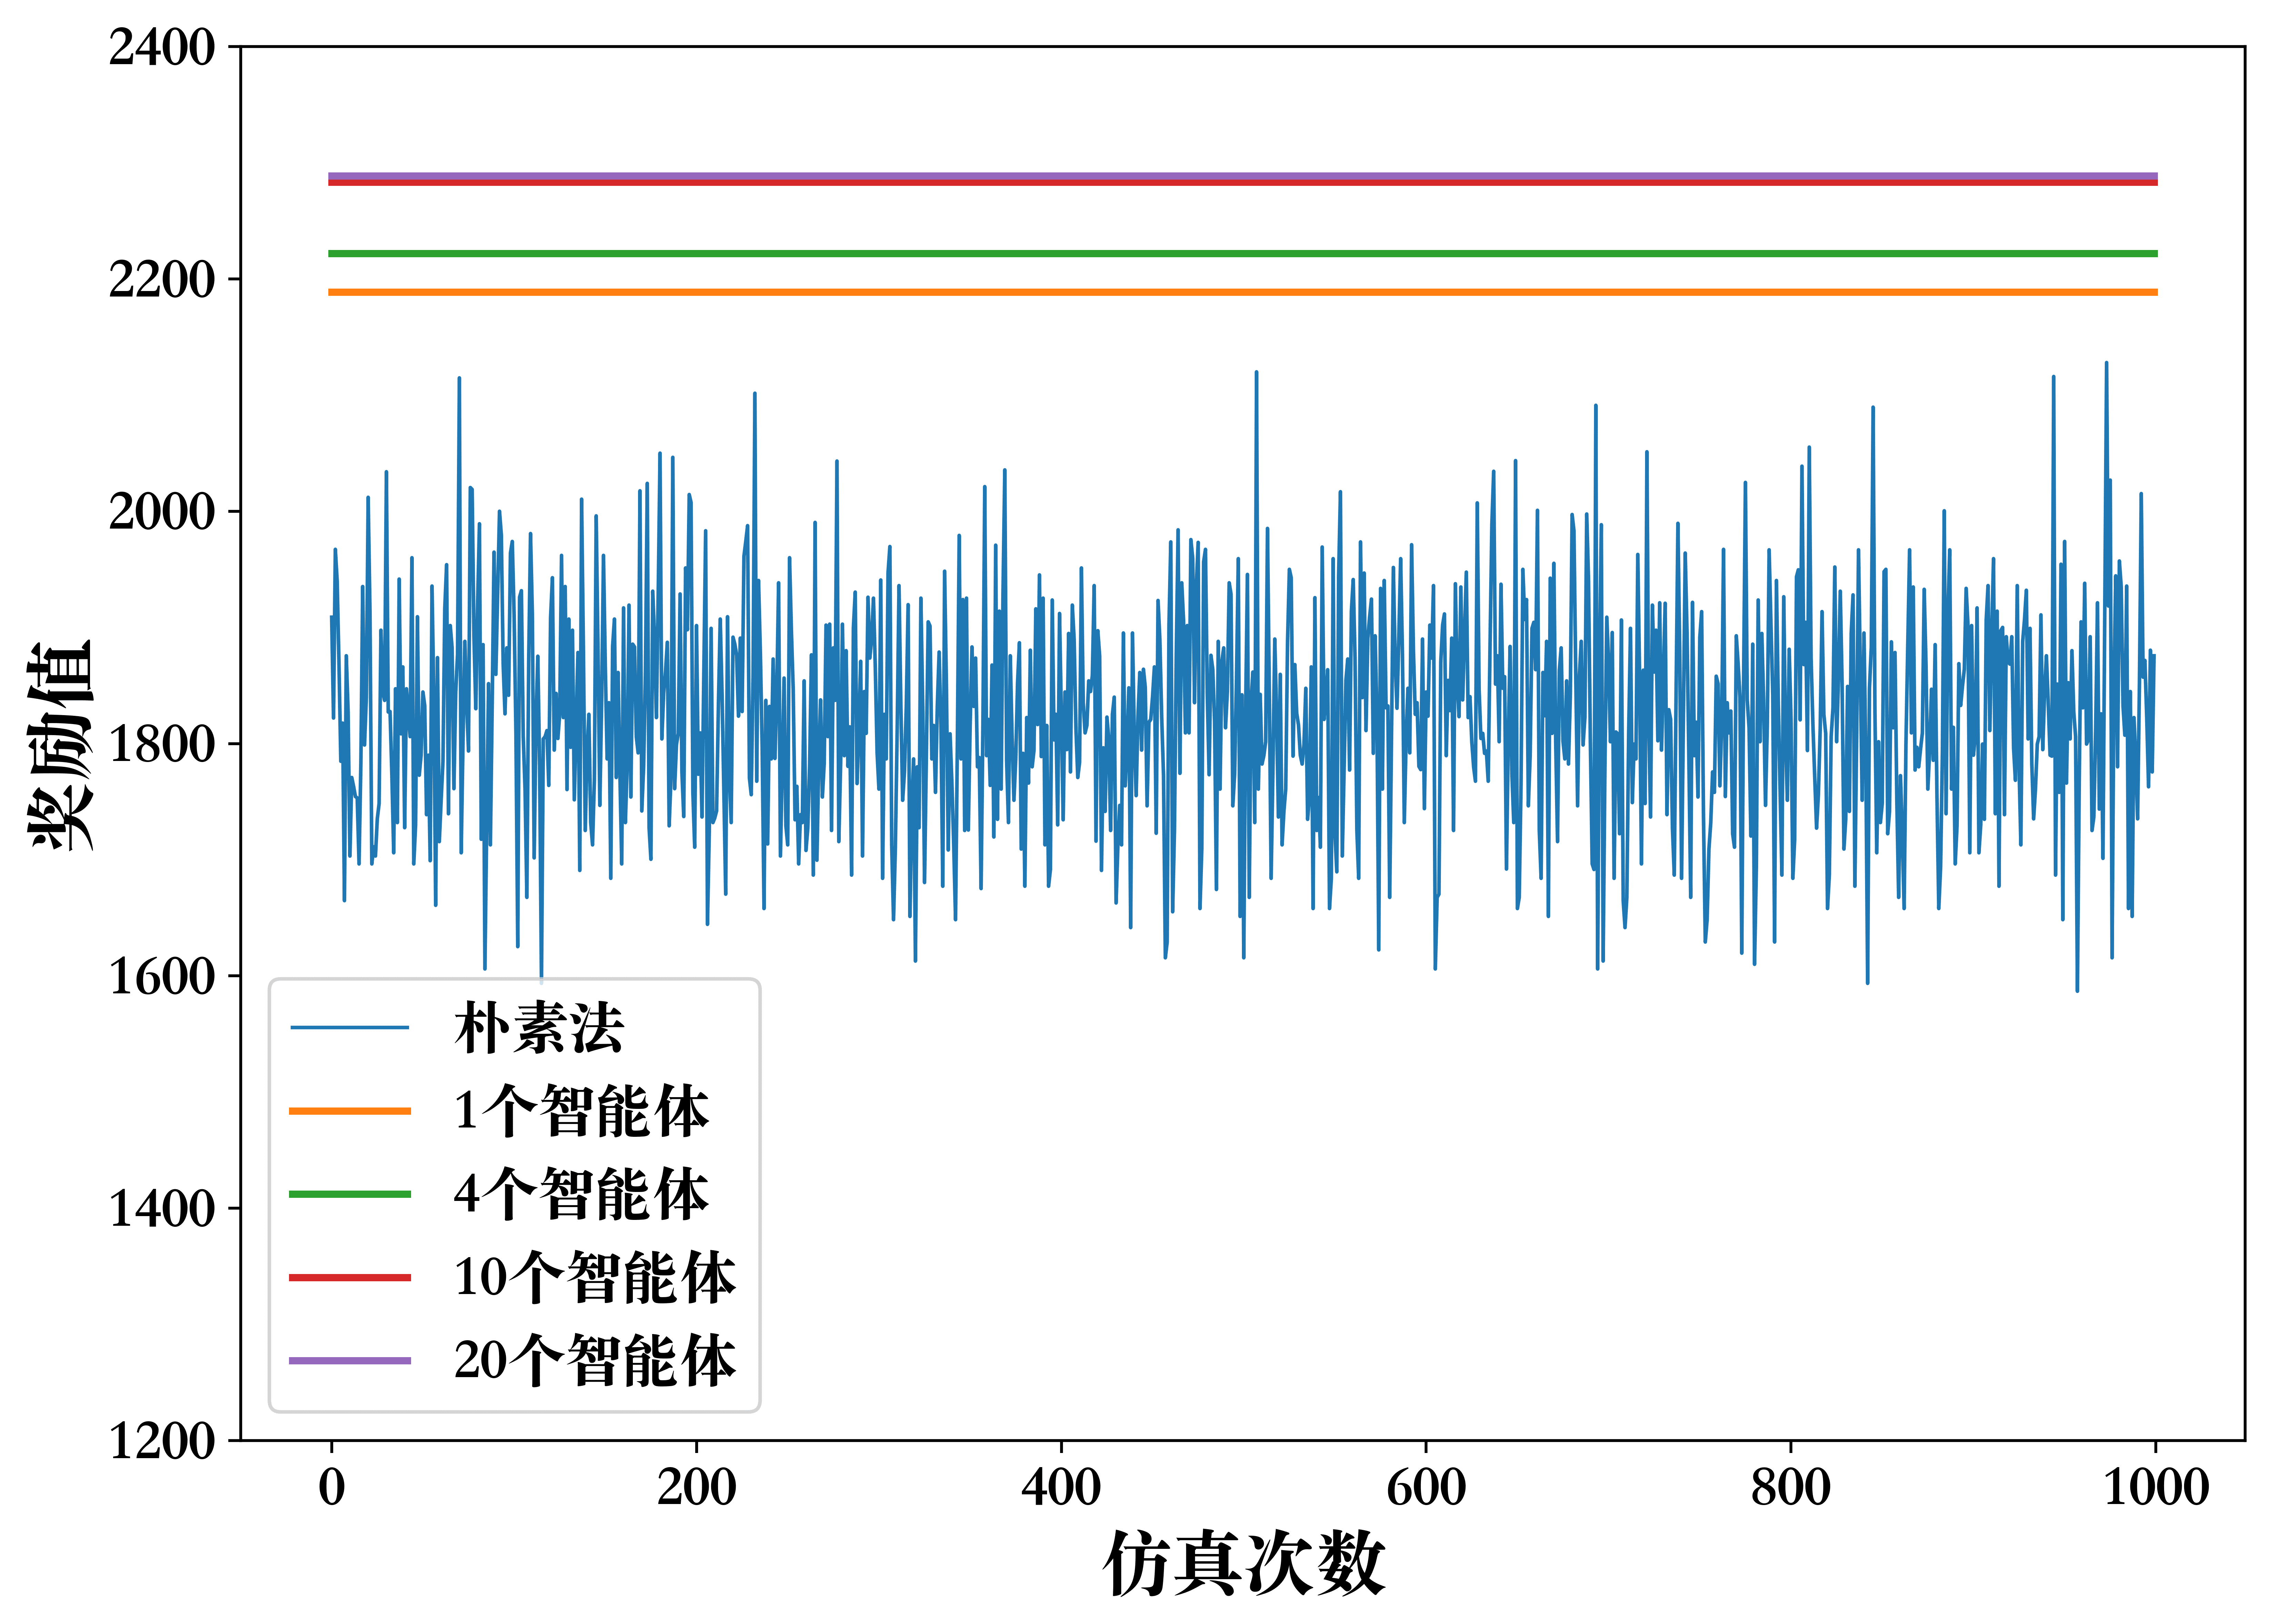
\includegraphics[width=.4\textwidth]{figures/content/size/size6.png}}
  \\
  \subfloat[智能体1]{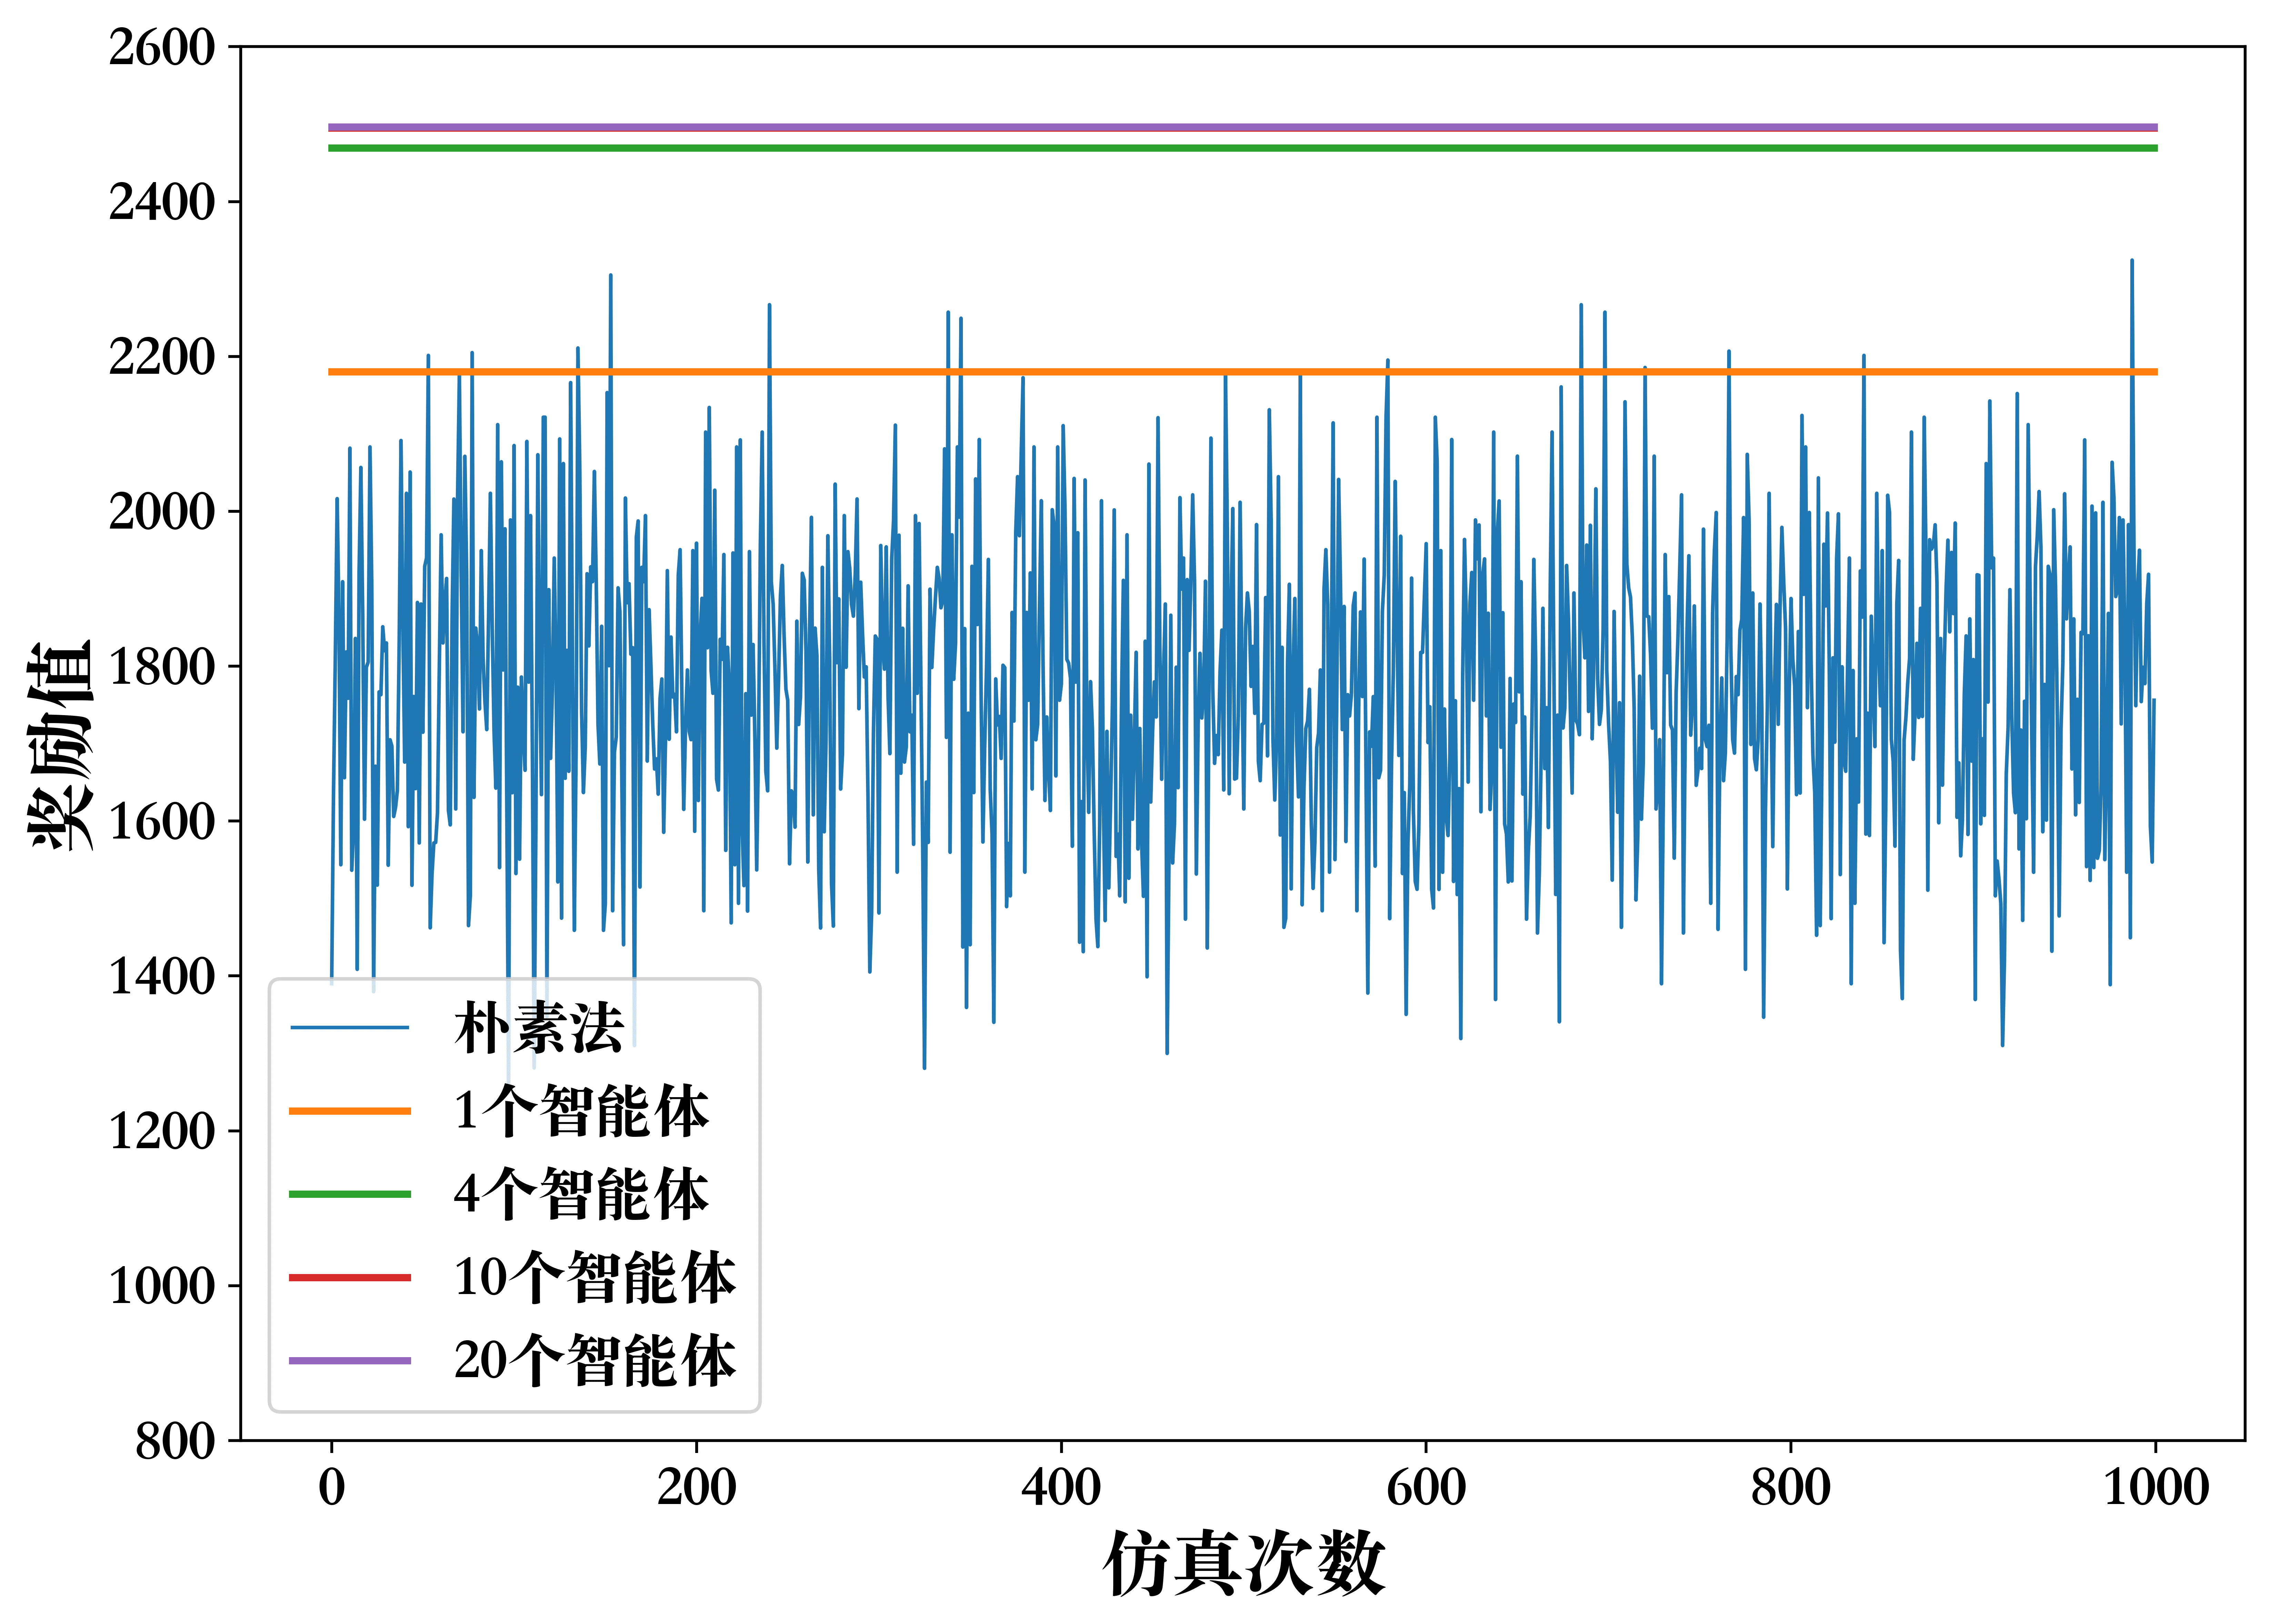
\includegraphics[width=.4\textwidth]{figures/content/size/size7.png}}
  \quad\quad
  \subfloat[智能体2]{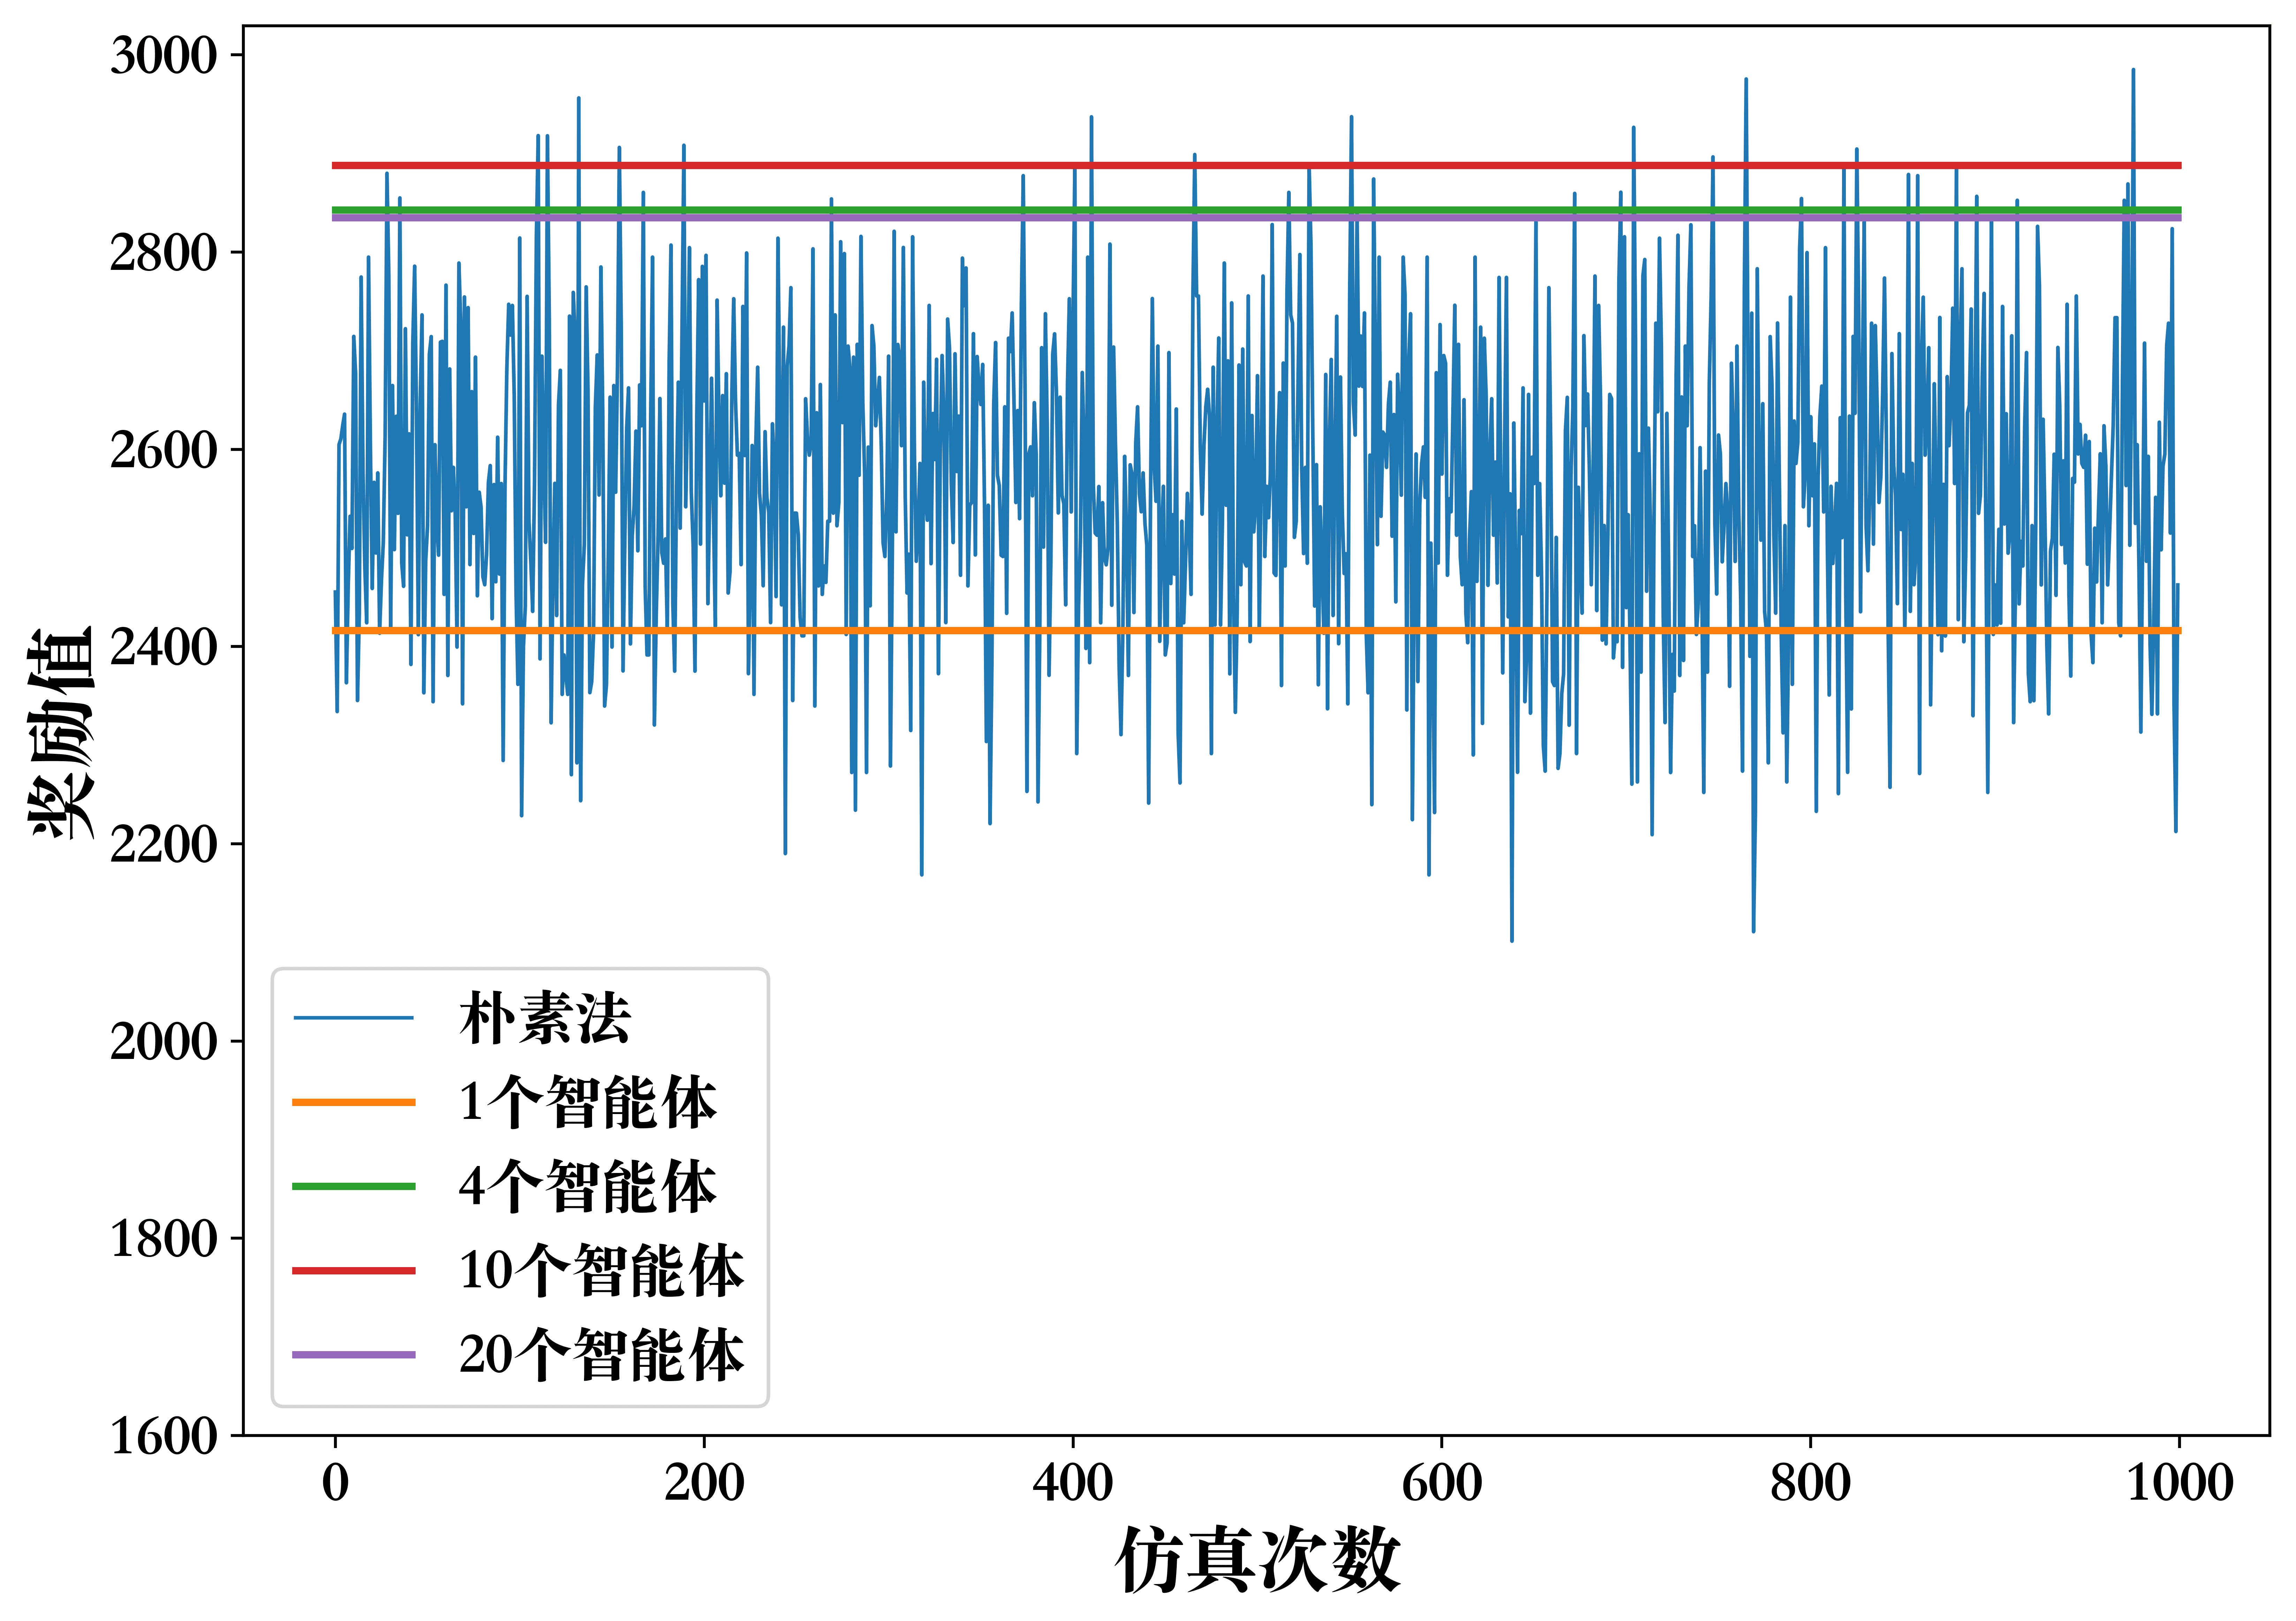
\includegraphics[width=.4\textwidth]{figures/content/size/size8.png}}
  \caption{训练过程中代表智能体的动作选择变化}
  \label{agents}
\end{figure}

\begin{table}[htbp]
\centering
\caption{使用不同的训练个体集时,所提出方法的性能变化。}
\label{cluster_agents}
\renewcommand{\arraystretch}{1.2}
\setlength{\tabcolsep}{6mm}
\small

\begin{tabular}{lccccc}
\toprule
               & 集合1   & 集合2    & 集合3    & 集合4        \\ 
\midrule
平均奖励 & 3,203 & 3,179 & 3,280 & 3,248           \\
超过95\%(共50个)    & 41        & 39         & 43         & 43         \\ 
\bottomrule
\end{tabular}
\end{table}
